% Customizable fields and text areas start with % >> below.
% Lines starting with the comment character (%) are normally removed before release outside the collaboration, but not those comments ending lines

% svn info. These are modified by svn at checkout time.
% The last version of these macros found before the maketitle will be the one on the front page,
% so only the main file is tracked.
% Do not edit by hand!
\RCS$Revision: 219929 $
\RCS$HeadURL: svn+ssh://svn.cern.ch/reps/tdr2/notes/AN-13-357/trunk/AN-13-357.tex $
\RCS$Id: AN-13-357.tex 219929 2013-12-08 10:26:50Z paktinat $
%%%%%%%%%%%%% local definitions %%%%%%%%%%%%%%%%%%%%%
% This allows for switching between one column and two column (cms@external) layouts
% The widths should  be modified for your particular figures. You'll need additional copies if you have more than one standard figure size.
\newcommand{\invfb}{\ensuremath{\,\rm{fb^{-1}}}\xspace}
\newcommand{\invpb}{\ensuremath{\,\rm{pb^{-1}}}\xspace}
\newcommand{\mt}{\ensuremath{\,{m_T}}\xspace}
\newcommand{\mttwo}{\ensuremath{\,{M_{T2}}}\xspace}
\newcommand{\met}{\ensuremath{\,{E_T^{miss}}}\xspace}
\newcommand{\mindphifour}{\ensuremath{\,{\Delta\phi_{4}^{min}}}\xspace}
\newcommand{\pT}{\ensuremath{\,p_T}\xspace}



\newlength\cmsFigWidth
\ifthenelse{\boolean{cms@external}}{\setlength\cmsFigWidth{0.85\columnwidth}}{\setlength\cmsFigWidth{0.4\textwidth}}
\ifthenelse{\boolean{cms@external}}{\providecommand{\cmsLeft}{top}}{\providecommand{\cmsLeft}{left}}
\ifthenelse{\boolean{cms@external}}{\providecommand{\cmsRight}{bottom}}{\providecommand{\cmsRight}{right}}
%%%%%%%%%%%%%%%  Title page %%%%%%%%%%%%%%%%%%%%%%%%
\cmsNoteHeader{AN-13-357} % This is over-written in the CMS environment: useful as preprint no. for export versions
% >> Title: please make sure that the non-TeX equivalent is in PDFTitle below
\title{A Hadronic Search for Direct Stop with MT2 Variable Using the Full 2012 Data}

% >> Authors
%Author is always "The CMS Collaboration" for PAS and papers, so author, etc, below will be ignored in those cases
%For multiple affiliations, create an address entry for the combination
%To mark authors as primary, use the \author* form
\address[ipm]{School of Particles and Accelerators, IPM, Tehran, Iran}
\address[ut]{University of Tehran, Tehran, Iran, also at IPM}
\address[iut]{Isfahan University of Technology, Isfahan, Iran, also at IPM}

\author[ipm]{Hamed Bakhshian}
\author[iut]{Shirin Chenarani}
\author[ipm]{Esmaeel Eskandari}
\author[ut]{Ali Fahim}
\author[ipm]{Abideh Jafari}
\author[ipm]{Saeid Paktinat Mehdiabadi}
\author[ipm]{Maryam Zeinali}

% >> Date
% The date is in yyyy/mm/dd format. Today has been
% redefined to match, but if the date needs to be fixed, please write it in this fashion.
% For papers and PAS, \today is taken as the date the head file (this one) was last modified according to svn: see the RCS Id string above.
% For the final version it is best to "touch" the head file to make sure it has the latest date.
\date{\today}

% >> Abstract
% Abstract processing:
% 1. **DO NOT use \include or \input** to include the abstract: our abstract extractor will not search through other files than this one.
% 2. **DO NOT use %**                  to comment out sections of the abstract: the extractor will still grab those lines (and they won't be comments any longer!).
% 3. For PASs: **DO NOT use tex macros**         in the abstract: CDS MathJax processor used on the abstract doesn't understand them _and_ will only look within $$. The abstracts for papers are hand formatted so macros are okay.
\abstract{A hadronic search for direct production of stops is performed on ~20 \invfb of data from 
proton-proton collision in the center of mass energy of 8 TeV at CMS. The most important backgrounds, are 
estimated using the data driven methods. 
It is shown that this analysis can access some parts of the SMS phase space which are not accessible by the \met analysis.
}

% >> PDF Metadata
% Do not comment out the following hypersetup lines (metadata). They will disappear in NODRAFT mode and are needed by CDS.
% Also: make sure that the values of the metadata items are sensible and are in plain text:
% (1) no TeX! -- for \sqrt{s} use sqrt(s) -- this will show with extra quote marks in the draft version but is okay).
% (2) no %.
% (3) No curly braces {}.
\hypersetup{%
pdfauthor={IPM MT2Top group},%
pdftitle={A Hadronic Search for Direct Stop with MT2 Variable Using the Full 2012 Data},%
pdfsubject={CMS},%
pdfkeywords={CMS, physics, software, computing}}

\maketitle %maketitle comes after all the front information has been supplied
% >> Text
%%%%%%%%%%%%%%%%%%%%%%%%%%%%%%%%  Begin text %%%%%%%%%%%%%%%%%%%%%%%%%%%%%
%% **DO NOT REMOVE THE BIBLIOGRAPHY** which is located before the appendix.
%% You can take the text between here and the bibiliography as an example which you should replace with the actual text of your document.
%% If you include other TeX files, be sure to use "\input{filename}" rather than "\input filename".
%% The latter works for you, but our parser looks for the braces and will break when uploading the document.
%%%%%%%%%%%%%%%
\section{Introduction}
\label{sect:introduction}
Supersymmetry \cite{Martin:1997ns} (SUSY) is one of the most promising extensions of the 
Standard Model of the elementary particles (SM) which solves both the 
quadratic divergencies and hierarchy problems simultaneously. It introduces a new symmetry between the bosons and fermions and 
for every particle a sparticle is defined which is exactly same, but differ in spin by 1/2.
Since the super particles are not discovered yet, the supersymmetry should be a broken symmetry. Various mechanisms are introduced to 
break the symmetry softly without changing the other interesting features of the theory.

A search for new physics using 5.1 \invfb of data from CMS taken in 2012 is documented in this note. Although the search is sensitive to any high scale 
new physics with a missing transverse momentum, R-parity conserving SUSY model is used to illustrate the performance of the method.

The search variable is the stransverse mass (\mttwo) which is the natural extension of the known transverse mass (\mt) to a case 
when two massive particles with equal mass are created in pairs and decay via a chain of jets and leptons to two invisible particles. 
In the case of R-Parity conserving SUSY, the Lightest Supersymmetric Particle (LSP) escapes the detection and appears as 
a missing transverse momentum.
The distribution of \mttwo reflects the scale of the produced particles and is much higher for sparticles
compared to the SM particles. Hence, SUSY should appear as an excess in the tail of the \mttwo distribution.
It was shown previously \cite{MT2_2011} that \mttwo is a powerful variable to search for SUSY. Due to consistency of the data with background 
only hypothesis, low mass gluino and squarks have been ruled out. A main direction suggested by the theoreticians and phenomenologists is to 
search for the third generation of the sparticles.% [Arkani Hamed]. 
Since the third generation of the SM particles are heavier than the first two generations, 
in the SUSY sector, this generation can be much lighter. The current analysis is optimized to search for the direct production of 
the supersymmetric partner of the top quark (stop) in the hadronic final states. It is assumed that the pair produced stops undertake the 
following decay chain:
\begin{linenomath}
\begin{equation}
\tilde{t} \rightarrow t + \tilde{\chi_{1}^{0}}
\end{equation}
\end{linenomath}
when top decays hadronically:
\begin{linenomath}
\begin{equation}
t \rightarrow b + W \rightarrow b + q + q'
\end{equation}
\end{linenomath}
and $\tilde{\chi_{1}^{0}}$ can not be detected and appears as \met.

After introduction in the next section the \mttwo variable is introduced. 
A sepcial method for top reconstruction is described in section \ref{sect:top}.
The data and MC samples are defined in section \ref{sect:dataMC}. 
Different physical objects used in this analysis are introduced in section \ref{sect:objdef}. 
Sections \ref{sect:trigger}-\ref{sect:cuts} review the procedure to 
select the trigger and cuts to have a better reach in this search.
Our strategy to search for stop is explained in section \ref{sect:search}.
Data driven methods are used to estimate the contribution of the main SM backgrounds. 
Section \ref{sect:bkg} shows the methods and their performance.
The statistical methods are used to interpret the results in section \ref{sect:stat} and finally section \ref{sect:conclusion} concludes the note.




%\section{The definition of $\rm {M_{T2}}$}
\section{\texorpdfstring{The definition of $\rm {M_{T2}}$}{The definition of MT2}}
\label{sect:mt2def}
The variable transverse masss is used to measure the mass of the W-boson~\cite{Arnison:1983rp,Banner:1983jy,Affolder:2000bpa,Abazov:2002bu} in its decay to a lepton and a neutrino, where only the transverse missing energy due to undetected neutrino could be measured. It is defined as 
\begin{linenomath}
\begin{equation}
\label{eq:mtdef}
m_{T}^{2}= 2\,( E_T^lE_T^\nu-\vec{p_T}^l.\vec{p_T}^\nu ),
\end{equation}
\end{linenomath}
where for neutrino, $E_T^\nu=p_T^\nu$. The kinmatic endpoint of $m_T$ is an estimator for the W-mass, i.e. $m_T^2\leq m_W^2$. \\
The $M_{T2}$ variable~\cite{Lester:1999tx,Barr:2003rg} is introduced and used in this analysis to discriminate between SUSY signal and the SM backgrounds while it is originally intended to estimate the mass of unseen particles. The kinematic endpoint of $M_{T2}$ carries model independent information about the mass difference between the primary and the secondary supersymmetric particles. It is in particular useful to study events containing two simultaneous decays of a supersymmetric particle into a visible and an undetectable particle (e.g. neutralino). It is defined as
\begin{linenomath}
\begin{equation}
\label{eq:mt2def}
M_{T2}(m_{\chi})= \min_{p_{T}^{\chi_1}+p_{T}^{\chi_2}=E_T^{miss}}\,\left[\,\max\,\{ \, m_{T}(p_T^{\chi_1};m_{\chi}),\,m_{T}(p_T^{\chi_2};m_{\chi})\,\}\,\right],
\end{equation}
\end{linenomath}
where $\chi$ stands for the neutralino whose mass is a free parameter in the evaluation of $M_{T2}$. The choice of maximum $m_T$ is reasonable since none of the two transverse mass exceeds the mass of parents. The chosen transverse mass is minimized over the range of $m_{\chi}$ which again ensures that $m_T$ is less than the parents mass. \\
While for boosted systems in the transverse plain $M_{T2}$ can be computed only numerically, there are analytic solutions~\cite{Cho:2007dh} for unboosted scenarios. There, one can write the $M_{T2}$ endpoint as a function of the masses. \\
To reconstruct the visible system as the input for $M_{T2}$ calculation, the visible part of the event (jets in this analysis) is decomposed into two \textit{pseudojets}. The procedure is known as \textit{hemisphere} reconstruction and is already used in~\cite{CMS-PAS-SUS-12-002}. The two massless jets with the highest invariant mass define the primary two directions of hemispheres. Other jets are added to one of the hemispheres based on the minimal Lund distance ( see e.g. ~\cite{Sjostrand:2006za}). The resulting $M_{T2}$ variable is proven to well reject the multi-jet processes with non-genuine $E_{T}^{miss}$~\cite{CMS-PAS-SUS-12-002}. \\

%{\bf FIXME For this round should be commented otherwise a short description is needed.}
%For the special case of $\tilde{t}$ as the primary sparticle decaying to $t+\tilde{\chi^0_1}$, the reconstruction of hadronically decaying 
%top quark can define the visible inputs for $M_{T2}$~\cite{MT2_2011}. The study of this top-based, $M_{T2}^{top}$, variable is presented in 
%Section~\ref{subsect:mt2top} where it is also tried to extract more discriminating quantities based on the first reconstructed top quark, 
%$E_T^{miss}$ and jets in the remaining (R) system. The proposed variables however fail to improve the exclusion limits.
%\subsection{\texorpdfstring{Top reconstruction and $\rm {M_{T2}^{top}}$}{Top reconstruction and MT2top}}
%\label{subsect:mt2top}
%Do we want to have this section? Or do we want to present their effect in cut optimization?


\section{Top Reconstruction}
\label{sect:top}
%{\bf FIXME We received some comments from Luc on Top finding purity. S}
To reconstruct top quarks a special method is used.  
The main features 
of the method are using a $\chi^2$ and mass of the jets. A $\chi^2$ is
constructed based on the known masses of $W$ and top, e.g.
\begin{linenomath}
\begin{equation}
\label{eq:chi2}
\chi^2 = \frac{(M_{2j} - M_W)^2}{\sigma^2_W} + \frac{(M_{3j} - M_t)^2}{\sigma^2_t}; 
\end{equation}
\end{linenomath}
$M_{2j}$ is usually the invariant mass of 2 jets making a $W$ boson, 
but it can also be a heavy single jet, and $M_{3j}$ is the invariant mass of 3 jets making a top quark. The uncertainty on invariant masses is computed as
\begin{linenomath}
\begin{equation}
\label{eq:sigma}
\sigma_x = \sqrt{\frac{1}{4}\sum_{i} \pod{\frac{\Delta p_i}{p_i}}^2\pod{\frac{\sum_{j \neq i} M_{ij}^2}{M}}^2 + \Gamma_x^2}; 
\end{equation}
\end{linenomath}
where $p_i$ uncertainty is taken as $\frac{\Delta p_i}{p_i} = \frac{100\%}{\sqrt{p_i}}$ and $\Gamma_x$ is the width of $W$ (2.1 GeV) 
and top (10 GeV). Top reconstruction is started by reconstructing all possible $W$'s from either 2 jets (W2j) or 1 heavy jet (W1j).
Solutions are kept only if they have a $\chi^2$ which is less than a fixed maximum value (2 in this analysis) for $W$ in W2j
and in W1j giving the $W$ mass in a small window (80.4 $\pm$ 10.0 GeV/$c^2$). To calculate the $\chi^2$ for W1j, the width ($\Gamma_x$) in 
Equation \ref{eq:sigma} is set equal to 10 GeV/$c^2$. If a heavy jet is in a given mass range and is $b$-tagged, 
it is considered as a coalescence of a $b$ with a jet from $W$ (W1b). The mass window for W1b is set to [40,130] GeV/$c^2$ . 
$\chi^2$ = 1 is assigned to W1b candidates to avoid any systematic decrease of $\chi^2$ for the top combinations containing such objects.
All reconstructed $W$'s are ordered in their $\chi^2$ value. In case of overlapping $W$'s, only the best $\chi^2$ solution is kept. 
In the next step, the reconstructed $W$'s are used to reconstruct the top candidates by adding a free jet. To reduce the correlations,
before using the $W$'s, their 4-vector is rescaled to give the correct $W$ mass (80.4 GeV/$c^2$). If there is any overlap between the tops, 
the combination with a correct $b$-tagged jet ($b$+$W$) or a W1b is preferred over the best $\chi^2$ solution. 

\subsection{Performance of the Algorithm}
%By efficiency we want to know how many of generated top quarks are found 
The number of generated top quarks which are found at the reconstruction level demonstrates the performance of the top search algorithm.
% with the “top search” algorithm. 
Only hadronically decaying top quarks are considered. The efficiency of the algorithm is defined as: 

$$\epsilon_{topSearch} = N_{reco-top}^{matched}  / N_{gen-top}^{hadronic}$$

where reconstructed top quarks are matched with generated ones if $\Delta R(top_{rec},top_{gen}) < 0.1$. The overall results are shown in Table \ref{tbltopreceff}.

\begin{table}[htb]
  \begin{center}
    \begin{tabular}{|c|c|c|c|c|}
      \hline
      \textbf{\#events}  &  \textbf{\#gen-top-hadronic}  &  \textbf{\#rec-top-all}  &  \textbf{\#rec-top-matched}  &  \textbf{Overall efficiency}  \\
      \hline
      1.16 ME          &                        2601  &                   1331  &                   936  &  36\%                  \\
      \hline
    \end{tabular}
    \caption{The total efficiency of the top reconstruction algorithm. The efficiency is defined as the fraction of the generated top quarks which are reconstruted by the top search algorithm.}
    \label{tbltopreceff}
  \end{center}
\end{table}

The efficiency versus different event kinematic variables is studied and the results are shown in Figure \ref{figtopref_eff}.
%Efficiency is investigated in different jet bins.
 The probability to find a hadronically decaying top is higher in higher jet multiplicities (Figure 1,top-left).

%The efficiency of the top reconstruction vs. number of b-tagged jets is also studied.
Although there is no constraint for the combination to contain a b-tagged jet, in case of a tagged jet in the top combination, it is preferred over minimum $\chi^2$. The efficiency is stable in Nb-jets bins, as expected. The last bin in Figure 1 (top-right) suffers from low statistics.

As the efficiency versus the top $\pT$ is shown in Figure \ref{figtopref_eff}, if top quarks are “generated” with higher $\pT$, there is a higher probability for them to be reconstructed by our algorithm.

This study shows that efficiency is stable in $\mttwo$ bins, apart from the last two bins which have few entries.

\begin{figure}[htbp] 
\centering
    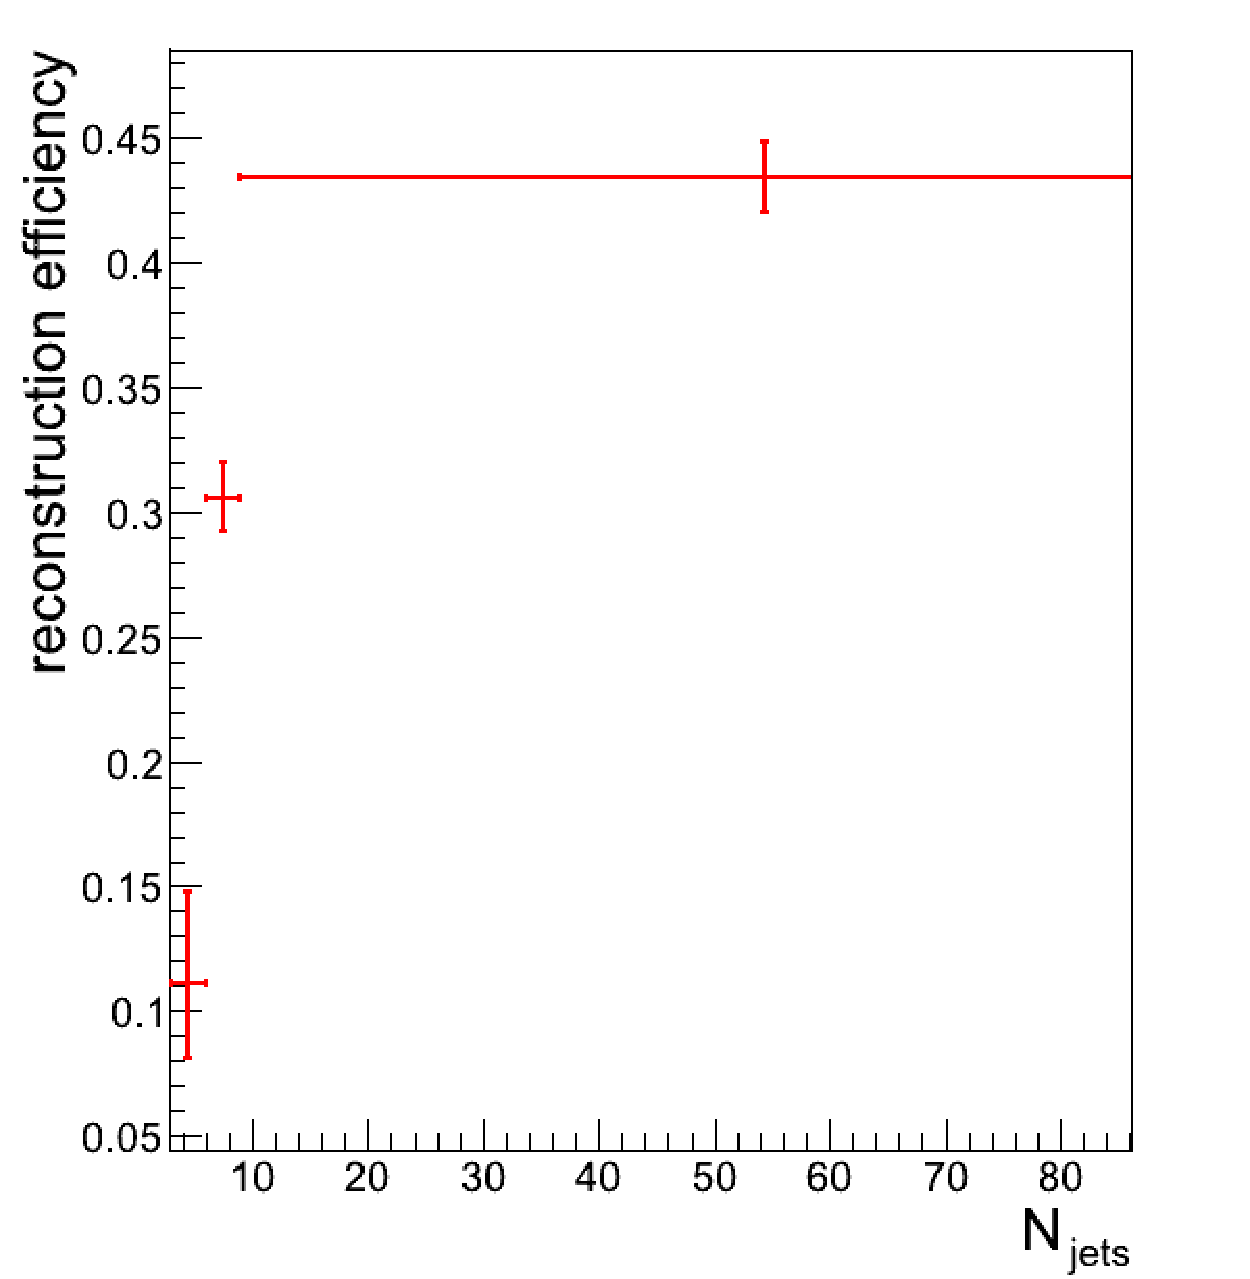
\includegraphics[width=0.3\textwidth]{figs/topNjet.pdf}
    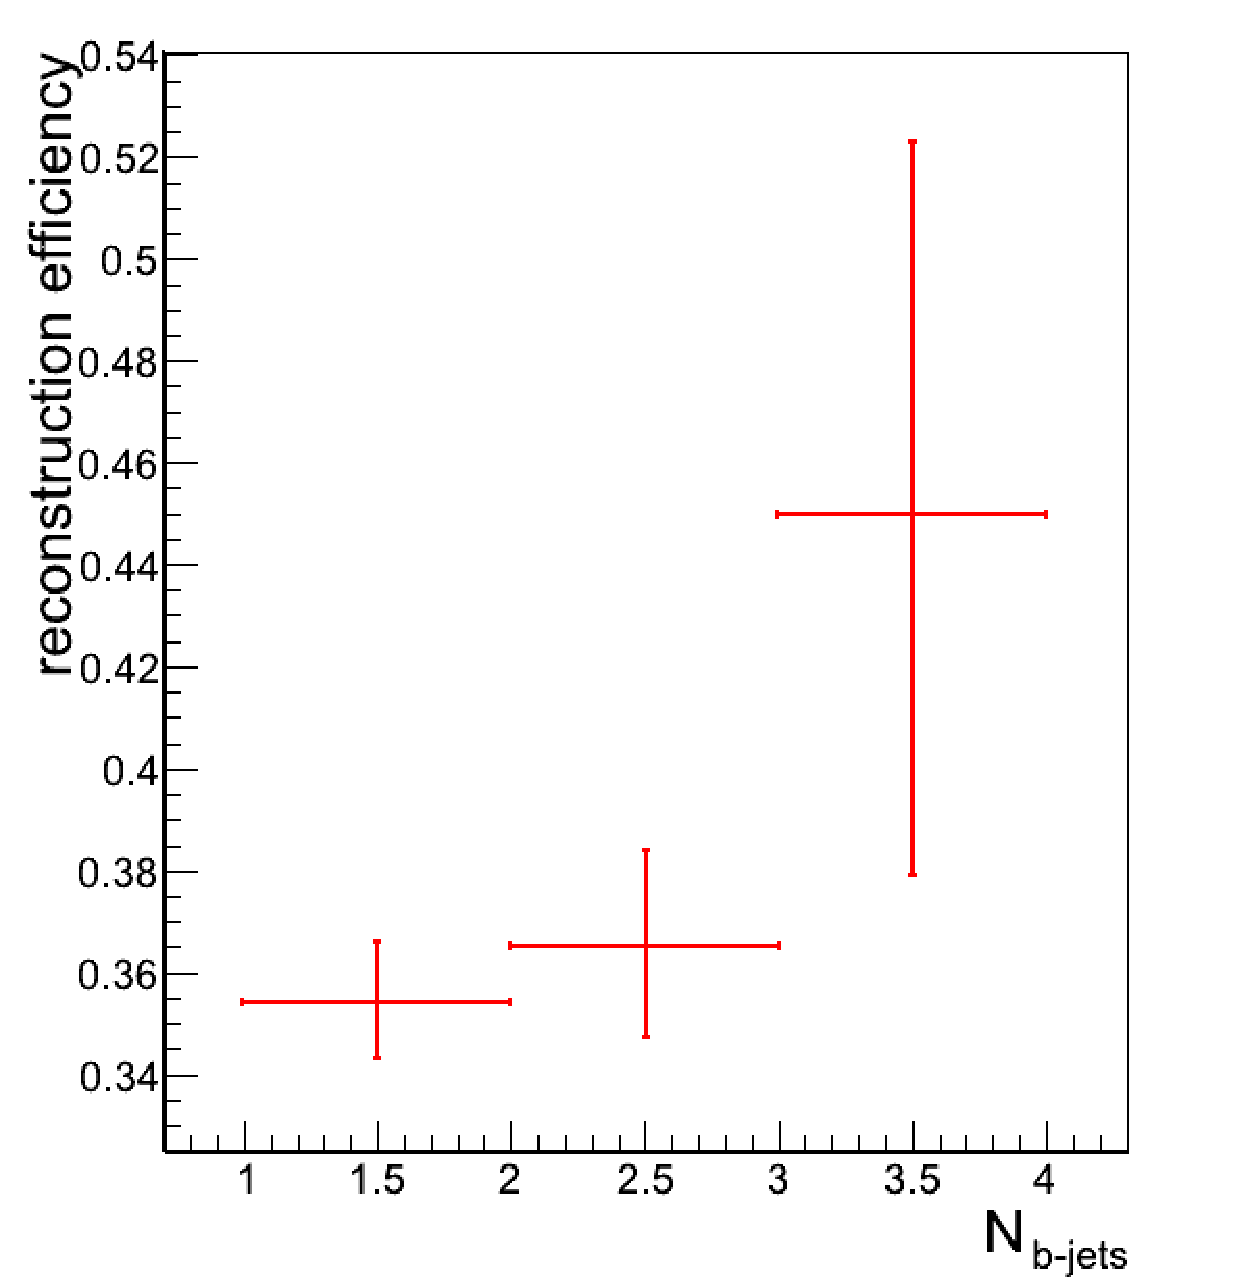
\includegraphics[width=0.3\textwidth]{figs/topNbjet.pdf} \\
    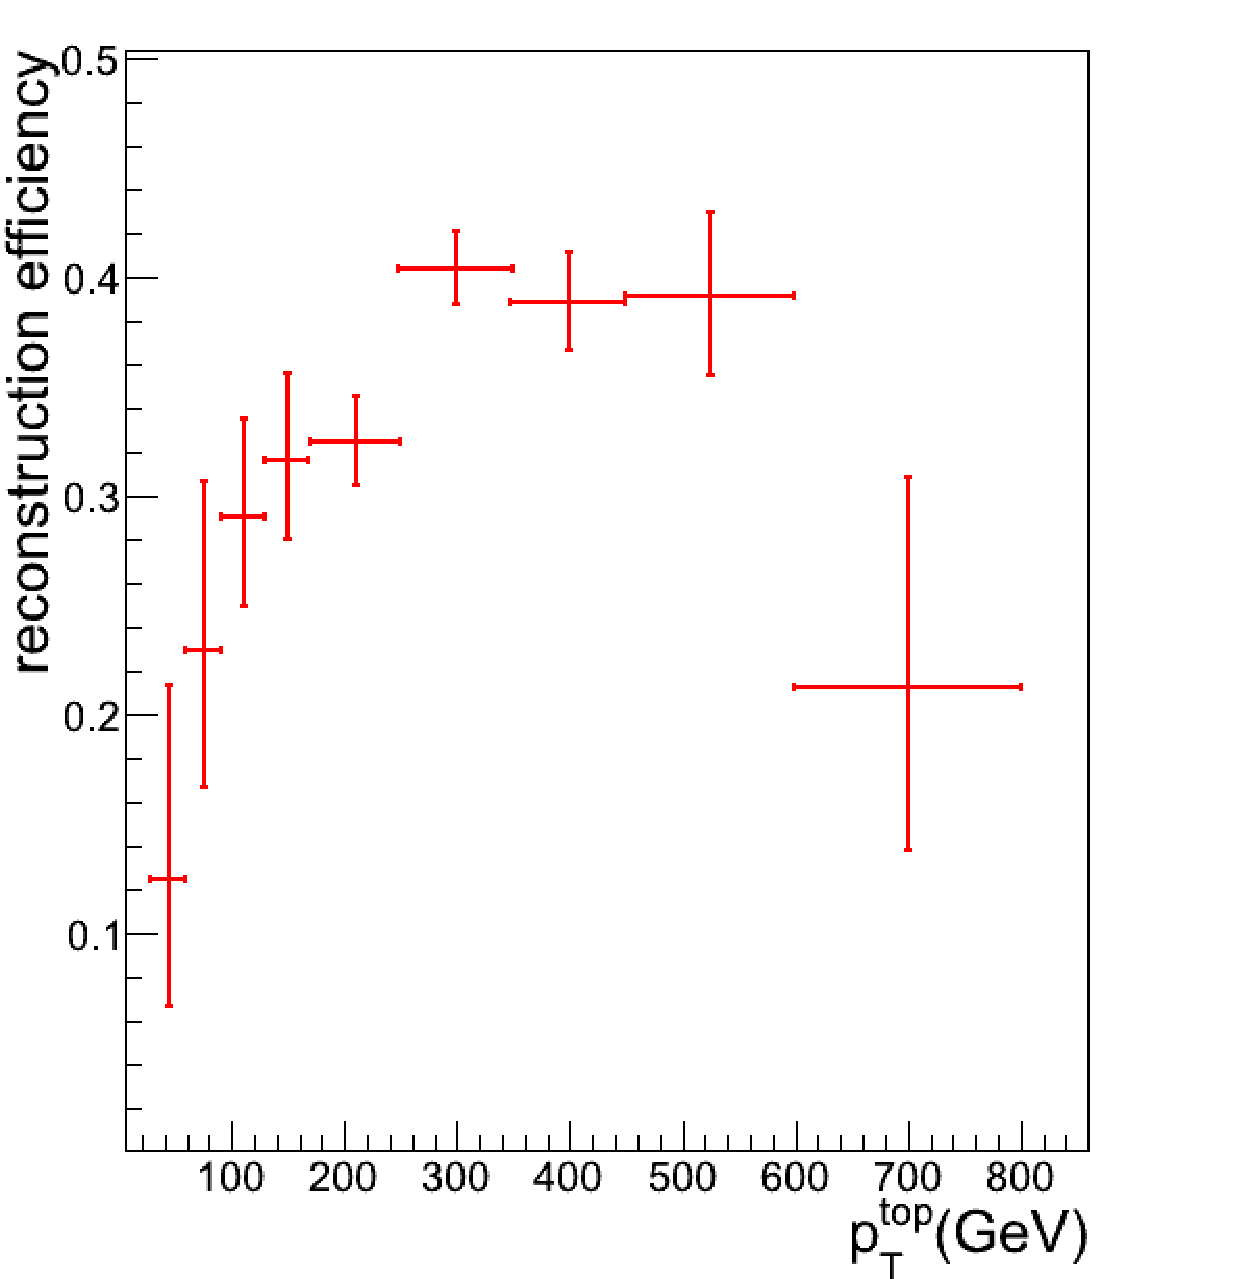
\includegraphics[width=0.3\textwidth]{figs/topPt.pdf}
    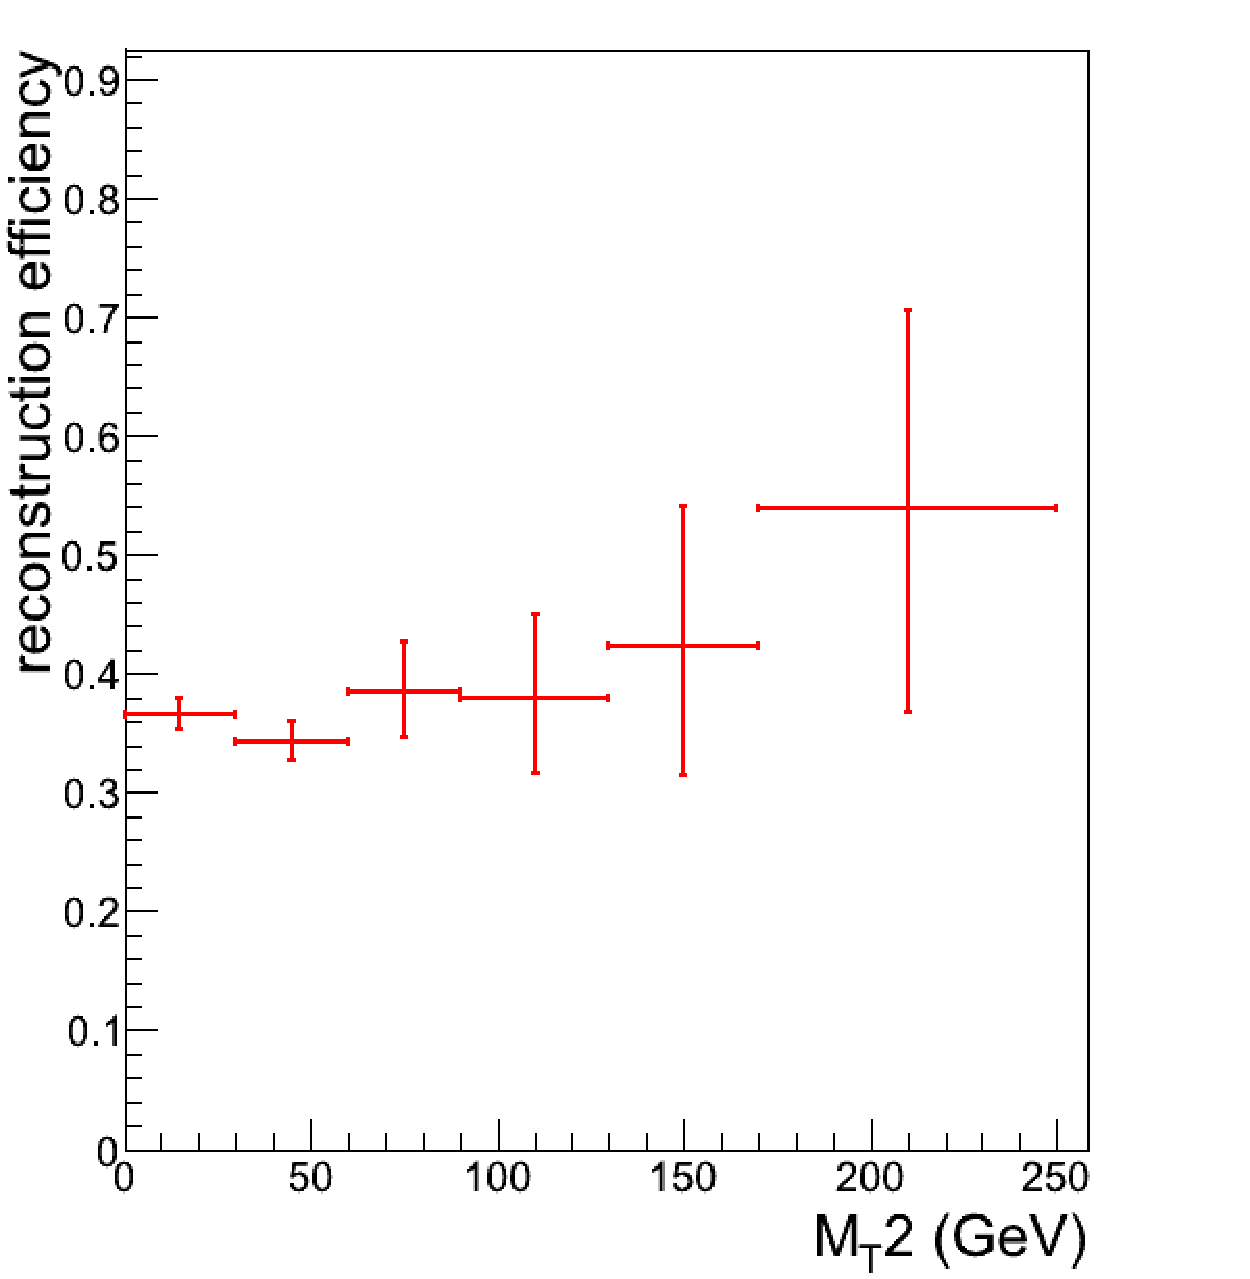
\includegraphics[width=0.3\textwidth]{figs/topMT2.pdf}
    \caption{The efficiency of top quark reconstruction algorithm is shown vs. number of jets (top-left) and number of
b-tagged jets (top-right), top $\pT$ (bottom-left) and $\mttwo$  and (bottom-right).}
    \label{figtopref_eff}
\end{figure}


The fake rate of the top reconstruction algorithm is also investigated. It is defined as the probability of reconstructing top from each 3 jets in a $W$ + jets event. So the ratio is normalized to the number of jets. The results after applying all MT2b cuts on the WJetsToLNu-HT-400ToInf-8TeV sample are shown in Figure \ref{figtopref_fake}. It can be see that the fake rate value is around $20\%$.


\begin{figure}[htbp] 
\centering
    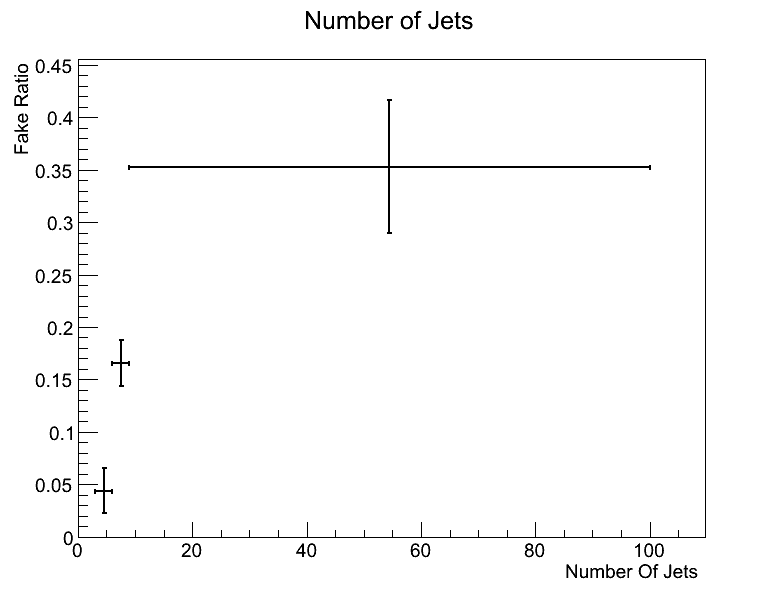
\includegraphics[width=0.3\textwidth]{figs/top_fake_NJets.png}
    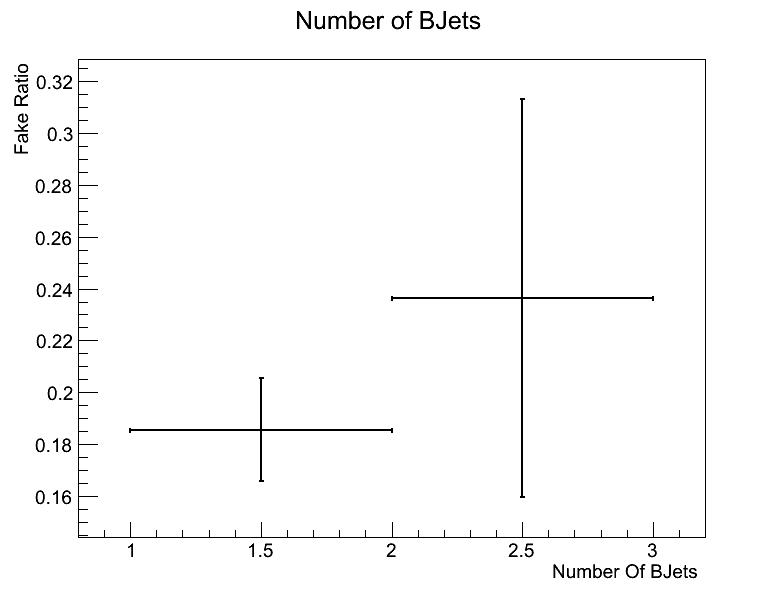
\includegraphics[width=0.3\textwidth]{figs/top_fake_NBJets.png} \\
    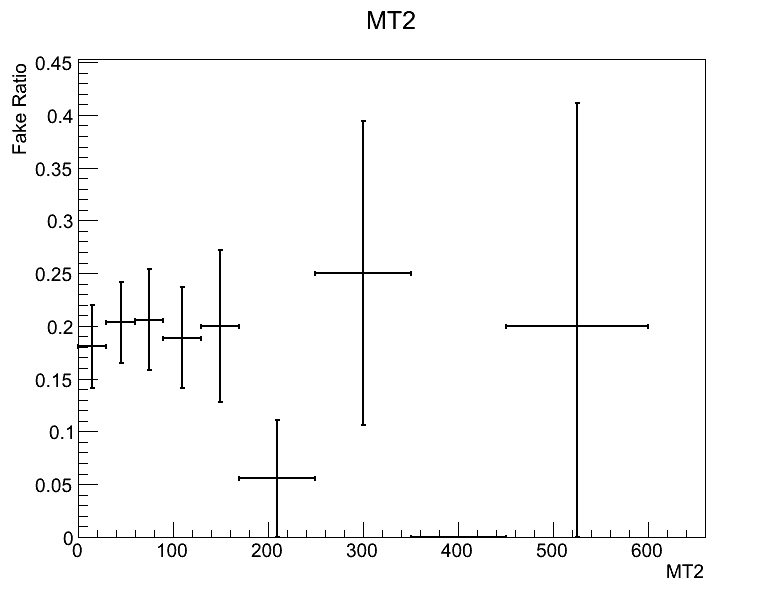
\includegraphics[width=0.3\textwidth]{figs/top_fake_MT2.png}
    \caption{The fake rate of the top reconstruction algorithm is shown vs. number of jets (top-left), number
of b-tagged jets (top-right) and $\mttwo$ (bottom).}
    \label{figtopref_fake}
\end{figure}

\section{Datasets and MC samples}
\label{sect:dataMC}
To reconstruct the objects, the CMSSW\_5\_3\_7\_patch5 is used for both data and MC.
The data used in the analysis corresponds to \IL of proton-proton collisions in the center of mass energy of $\sqrt{s}$ = 8 TeV 
which was taken in 2012. The list of the datasets, the run range and the corresponding integrated luminosities are as follow:
\begin{itemize}
\item /MultiJet/Run2012A-13Jul2012-v1/AOD (190456-193621, 952.6 \invpb) 
\item /MultiJet/Run2012A-recover-06Aug2012-v1/AOD (190782-190949, 95.4 \invpb) 
\item /MultiJet/Run2012B-13Jul2012-v1/AOD (193834-196531, 4.94 \invfb)
\item /MultiJet/Run2012C-24Aug2012-v1/AOD (198022-198523, 520.4 \invpb)
\item /MultiJet/Run2012C-PromptReco-v2/AOD (198941-203742, 6.9 \invfb)
\item /MultiJet/Run2012D-PromptReco-v1/AOD (203777-208686, 7.7 \invfb)
\end{itemize}

Only the lumisections with fully operative CMS subdetectors are used in this analysis (golden JSON files). To optimize the search method, MC 
samples are used for different Standard Model backgrounds and signals. These samples are officially generated and reconstructed by the CMS
collaboration. The full list of the samples and their cross sections are given in Table \ref{Tab.MCSamples}. For most of the samples the most 
accurate calculation of the cross sections available in the literature (usually NLO and NNLO) are used.The contribution from the diboson  samples was found to be very small.

\begin{table}[!htb]
\begin{center}
\caption{List of the MC samples used in this analysis.}
\label{Tab.MCSamples}
\begin{tabular}{|l|c|}
\hline
Sample name                                                                    & $\sigma$ (pb) \\\hline
QCD &  \\\hline
QCD-HT-100To250-TuneZ2star-8TeV-madgraph-pythia- &\\
~~~~Summer12-DR53X-PU-S10-START53-V7A-v1    & 10360000 \\
QCD-HT-250To500-TuneZ2star-8TeV-madgraph-pythia6-...-2  & 276000 \\
QCD-HT-500To1000-TuneZ2star-8TeV-madgraph-pythia6-...-2 & 8426 \\
QCD-HT-1000ToInf-TuneZ2star-8TeV-madgraph-pythia6-...-2 & 204 \\\hline

%QCD-Pt-120to170-TuneZ2star-8TeV-pythia6- & \\
%~~~~~~~Summer12-DR53X-PU-S10-START53-V7A-v3   & 156293.3\\
%QCD-Pt-170to300-TuneZ2star-8TeV-pythia6-v2-...-v1& 34138.15\\
%QCD-Pt-300to470-TuneZ2star-8TeV-pythia6-v3-...-v1& 1759.55\\
%QCD-Pt-470to600-TuneZ2star-8TeV-pythia6-...-v2   & 113.88 \\
%QCD-Pt-600to800-TuneZ2star-8TeV-pythia6-...-v2   & 26.99\\
%QCD-Pt-800to1000-TuneZ2star-8TeV-pythia6-...-v2  & 3.55\\
%QCD-Pt-1000to1400-TuneZ2star-8TeV-pythia6-...-v1 & 0.74\\
%QCD-Pt-1400to1800-TuneZ2star-8TeV-pythia6-...-v1 & 0.034\\
%QCD-Pt-1800-TuneZ2star-8TeV-pythia6-...-v1       & 0.0018\\\hline

Top &  \\\hline
T-t-channel-TuneZ2star-8TeV-powheg-tauola-...-v3    & 56.4\\ % 47\\
Tbar-t-channel-TuneZ2star-8TeV-powheg-tauola-...    & 30.7 \\%25.00\\
T-tW-channel-DR-TuneZ2star-8TeV-powheg-tauola-...   & 22.4 \\%10.7\\
Tbar-tW-channel-DR-TuneZ2star-8TeV-powheg-tauola-...& 11.1773\\%10.7\\
T-s-channel-TuneZ2star-8TeV-powheg-tauola-...       & 3.79\\%2.82\\
Tbar-s-channel-TuneZ2star-8TeV-powheg-tauola-...    & 1.76\\% 1.57\\

TTJets-MassiveBinDECAY-TuneZ2star-8TeV-madgraph-tauola- & \\
~~~~~~~Summer12-DR53X-PU-S10-START53-V7A-v1                & 245.8\\% 234\\
TTGJets-8TeV-madgraph-Summer12-DR53X-PU-S10-START53-V19-v1 & 2.166\\
TTH-Inclusive-M-125-8TeV-pythia6-Summer12-DR53X-PU-S10-START53-V7A-v1 &	0.130\\
TTWJets-8TeV-madgraph-Summer12-DR53X-PU-S10-START53-V7A-v1 & 0.232\\
TTWWJets-8TeV-madgraph-Summer12-DR53X-PU-S10-START53-V7A-v1 & 0.002037\\
TTZJets-8TeV-madgraph-v2-Summer12-DR53X-PU-S10-START53-V7A-v1 & 0.2057\\\hline

WJets& \\\hline

WJetsToLNu-HT-250To300-8TeV-madgraph &\\
~~~~~Summer12-DR53X-PU-S10-START53-V7A-v1                                    & 57.26 \\
WJetsToLNu-HT-300To400-8TeV-madgraph-...                                       & 45.68  \\
WJetsToLNu-HT-400ToInf-8TeV-madgraph-...                                       & 30.08 \\
WJetsToLNu-HT-200To250-8TeV-madgraph-...-V7C-v1                                & 90.27 \\\hline

ZJets & \\\hline
DYJetsToLL-M-10To50filter-8TeV-madgraph-... & \\
Summer12-DR53X-PU-S10-START53-V7A-v1             & 876.8\\
DYJetsToLL-M-50-TuneZ2Star-8TeV-madgraph-tarball-  ...              & 3503.71\\
ZJetsToNuNu-50-HT-100-TuneZ2Star-8TeV-madgraph-ext-...              & 452.75\\
ZJetsToNuNu-200-HT-400-TuneZ2Star-8TeV-madgraph-ext-...             & 49.28\\
ZJetsToNuNu-400-HT-inf-TuneZ2Star-8TeV-madgraph-ext-...             & 6.26\\
ZJetsToNuNu-100-HT-200-TuneZ2Star-8TeV-madgraph-ext-...V7C-v1          & 190.39\\\hline

SMS & \\\hline
SMS-T2tt-mStop-150to350-mLSP-0to250-8TeV-Pythia6Z- &\\
~~~~~Summer12-START52-V9-FSIM-v1-2 & \\

%SMS-T2tt-mStop-150to350-mLSP-0to250-8TeV-Pythia6Z- & \\
%~~~~~~~Summer12-START52-V9-FSIM-v1-2          &  \\
%SMS-T2tt-mStop-375to475-mLSP-0to375-8TeV-Pythia6Z-...          &  \\
%SMS-T2tt-mStop-500to650-mLSP-0to225-8TeV-Pythia6Z-...          &  \\
%SMS-T2tt-mStop-500to650-mLSP-250to550-8TeV-Pythia6Z-...        &  \\
%SMS-T2tt-mStop-675to800-mLSP-0to275-8TeV-Pythia6Z-...          &  \\
%SMS-T2tt-mStop-675to800-mLSP-300to700-8TeV-Pythia6Z-...        &  \\

\hline
\end{tabular}
\end{center}
\end{table}



\section{Physics Object Definition and Preselections}
\label{sect:objdef}
This section, describes the physics objects used in this analysis. 
\subsection{PF Jets}
\begin{itemize}
\item PF jets with $p_T>20$ GeV and $|\eta|<2.4$ are kept for the analysis.
\item Jets are required to pass loose pf-jet id cuts listed below:
\begin{itemize}
\item Number of constituents $>$ 1,
\item Neutral hadronic fraction $<$ 0.99,
\item Neutral electromagnetic fraction $<$ 0.99,
\item Charged hadronic fraction $>$ 0,
\item Charged electromagnetic fraction $<$ 0.99,
\item Charged multiplicity $>$ 0.
\end{itemize}
\end{itemize}
\subsection{PF Electrons}
\begin{itemize}
\item PF electrons with $p_T>10$ GeV and $|\eta|<2.4$ are selected with ECAL gap veto.
\item Electrons are required to pass cut-based electron id cuts corresponding to VBTF 95 working point, which is used for veto~\cite{eIDs}. These set of cuts contain the requirements on $|d0|<0.04$ cm and $|dz|<0.2$ cm, for which both of them are calculated with respect to the primary vertex. 
\item Combined relative PF isolation below 0.15.
\end{itemize}
\subsection{PF Muons}
\begin{itemize}
\item PF muons with $p_T>10$ GeV and $|\eta|<2.4$ are selected, which are asked to be global muons.
\item Normalized $\chi^2$ is required to be below 10.
\item At least one valid track hit and at lease one valid pixel hit is required.  
\item Number of chambers with matched segments is required to be greater than one and number of silicon layers should be above 5. 
\item Cuts on the $|d0|<0.2$ cm and the $|dz|<0.5$ cm, both with respect to the primary vertex, are applied.
\item Combined relative PF isolation below 0.2.
\end{itemize}


\subsection{PF Taus}
\label{sec:taus}
In this note taus always mean hadronically decaying taus, unless stated otherwise.
\begin{itemize}
\item Hadron Plus Strip (HPS) algorithm identified PF-taus
\item $p_\mathrm{T} > 20$ GeV and  $|\eta| <$ 2.3
\item A decay into one or three prongs, plus eventually a $\pi^0$, is required
\item Loose Electron Rejection: electron pion MVA discriminator $< 0.6$
\item Tight Muon Rejection: Tau Lead Track not matched to chamber hits, and no DT, CSC or RPC Hits in last 2 stations, and large enough energy deposit in ECAL + HCAL in 1 prong + 0 strip decay mode ($\sum$(ECAL+HCAL) $> 0.2 \cdot p_{\mathrm{T}}$.
\item Loose Isolation ($\Delta\beta$-corrected): $\Delta\beta$-corrected $\sum p_\mathrm{T}$ of PF charged and PF gamma isolation candidates ($p_\mathrm{T} > 0.5$ GeV) less than 2 GeV (in a cone of $\Delta R = 0.3$ around the tau axis), requiring 3 hits on tracks of charged isolation candidates.
\end{itemize}

\subsection{\texorpdfstring{PF \met}{PF MET}}
\begin{itemize}
\item Type1 corrected PF \met is used.
\end{itemize}
\subsection{Preselection}
\label{subsect:presel}
\begin{itemize}
\item At least one good vertex, with $\rho<2$ cm and $\abs z<24$ cm and Ndof $>4$ is requested.
\item There are some cleaning cuts which are applied against instrumental effects, including those listed below:
\begin{itemize}
\item An isolation based HBHE noise filter is applied,
\item Events identified as beam halo are filtered.
\end{itemize}
\end{itemize}

\subsection{MT2b Cuts}
\label{subsect:mt2bcuts}
This section provides a review on the cuts which are started with to study the triggers. This set of cuts are those mainly used in the $\rm MT2b$ analysis~\cite{MT2_2011}. Once the trigger is fixed, the optimized set of selection cuts which are used in the main stream of the current analysis will be described in detail in Section~\ref{sect:cuts}.
\begin{itemize}
\item The preselection cuts which was outlined in Section~\ref{subsect:presel}.
\item At least 4 jets with $p_T>40$ GeV and $\abs\eta<2.4$ are required which are asked to pass loos pf-jet id cuts.
\item The leading jet-$p_T$ should be greater than $150$ GeV.
\item It is also required that each jet with $p_T>50$ GeV to pass loos pf-jet id cuts.
\item At least one b-quark jet is requested with $p_T>20$ GeV within the tracker acceptance, which is tagged by the Simple Secondary Vertex algorithm with a tight working point.
\item The difference between \met and the vectorial $p_T$ sum of the selected jets, electrons and muons should be below $70$ GeV.
\item \met is required to be greater than $30$ GeV.
\item The minimum $\Delta\phi$ between \met and the four leading jets, hereafter referred to as \mindphifour, should be greater than $0.3$. There is no requirement on the id or $p_T$ of the jets when looking for the minimum azimuthal angle between \met and jets.
\item A cut on \mttwo $>$ 125 GeV is applied.
\item Leptons, being either electrons or muons, are vetoed.
\end{itemize}

\section{Trigger}
\label{sect:trigger}
\subsection{Trigger Study}
\label{sect:triggerstudy}
To have the best reach, two sets of triggers are compared. Their names and run ranges are shown in 
Table \ref{Tab.TriggerPaths}. The corresponding prescaled triggers which are used to find the trigger plateau are also shown.

\begin{table}[!htb]
\begin{center}
\caption{On line triggers, their references and run ranges. A logical OR between SixJet and QuadJet is used.}
\label{Tab.TriggerPaths}
\begin{tabular}{|l|l|c|}
\hline
\multicolumn{3}{|c|}{HT}\\
\hline
Trigger Path & Prescaled Trigger & Run Range \\\hline
HLT\_PFHT650\_v5 & HLT\_PFHT350\_v3 & 190650-190750\\
HLT\_PFHT650\_v6 & HLT\_PFHT350\_v4 & 191000-191400\\ 
HLT\_PFHT650\_v7 & HLT\_PFHT350\_v5 & 191500-193750\\ 
HLT\_PFHT650\_v8 & HLT\_PFHT350\_v6 & 193750-196030\\ 
HLT\_PFHT650\_v9 & HLT\_PFHT350\_v7 & 196046-196531\\ 
\hline
\multicolumn{3}{|c|}{MultiJet}\\
\hline
HLT\_SixJet45\_v1  & HLT\_SixJet35\_v1  & 190456 - 190738\\
HLT\_SixJet45\_v2  & HLT\_SixJet35\_v2  & 190782 - 196027\\
HLT\_SixJet45\_v3  & HLT\_SixJet35\_v3  & 196046 - 196531\\
HLT\_QuadJet80\_v1 & HLT\_QuadJet70\_v1 & 190456 - 190738\\
HLT\_QuadJet80\_v2 & HLT\_QuadJet70\_v2 & 190782 - 196027\\
HLT\_QuadJet80\_v3 & HLT\_QuadJet70\_v3 & 196046 - 196531\\
\hline
\end{tabular}
\end{center}
\end{table}

To take into account the statistics (the peak of the selected events by the un-prescaled trigger figure \ref{fig.TriggerPlateau} (middle)),
\begin{figure}[!htb]
\centering
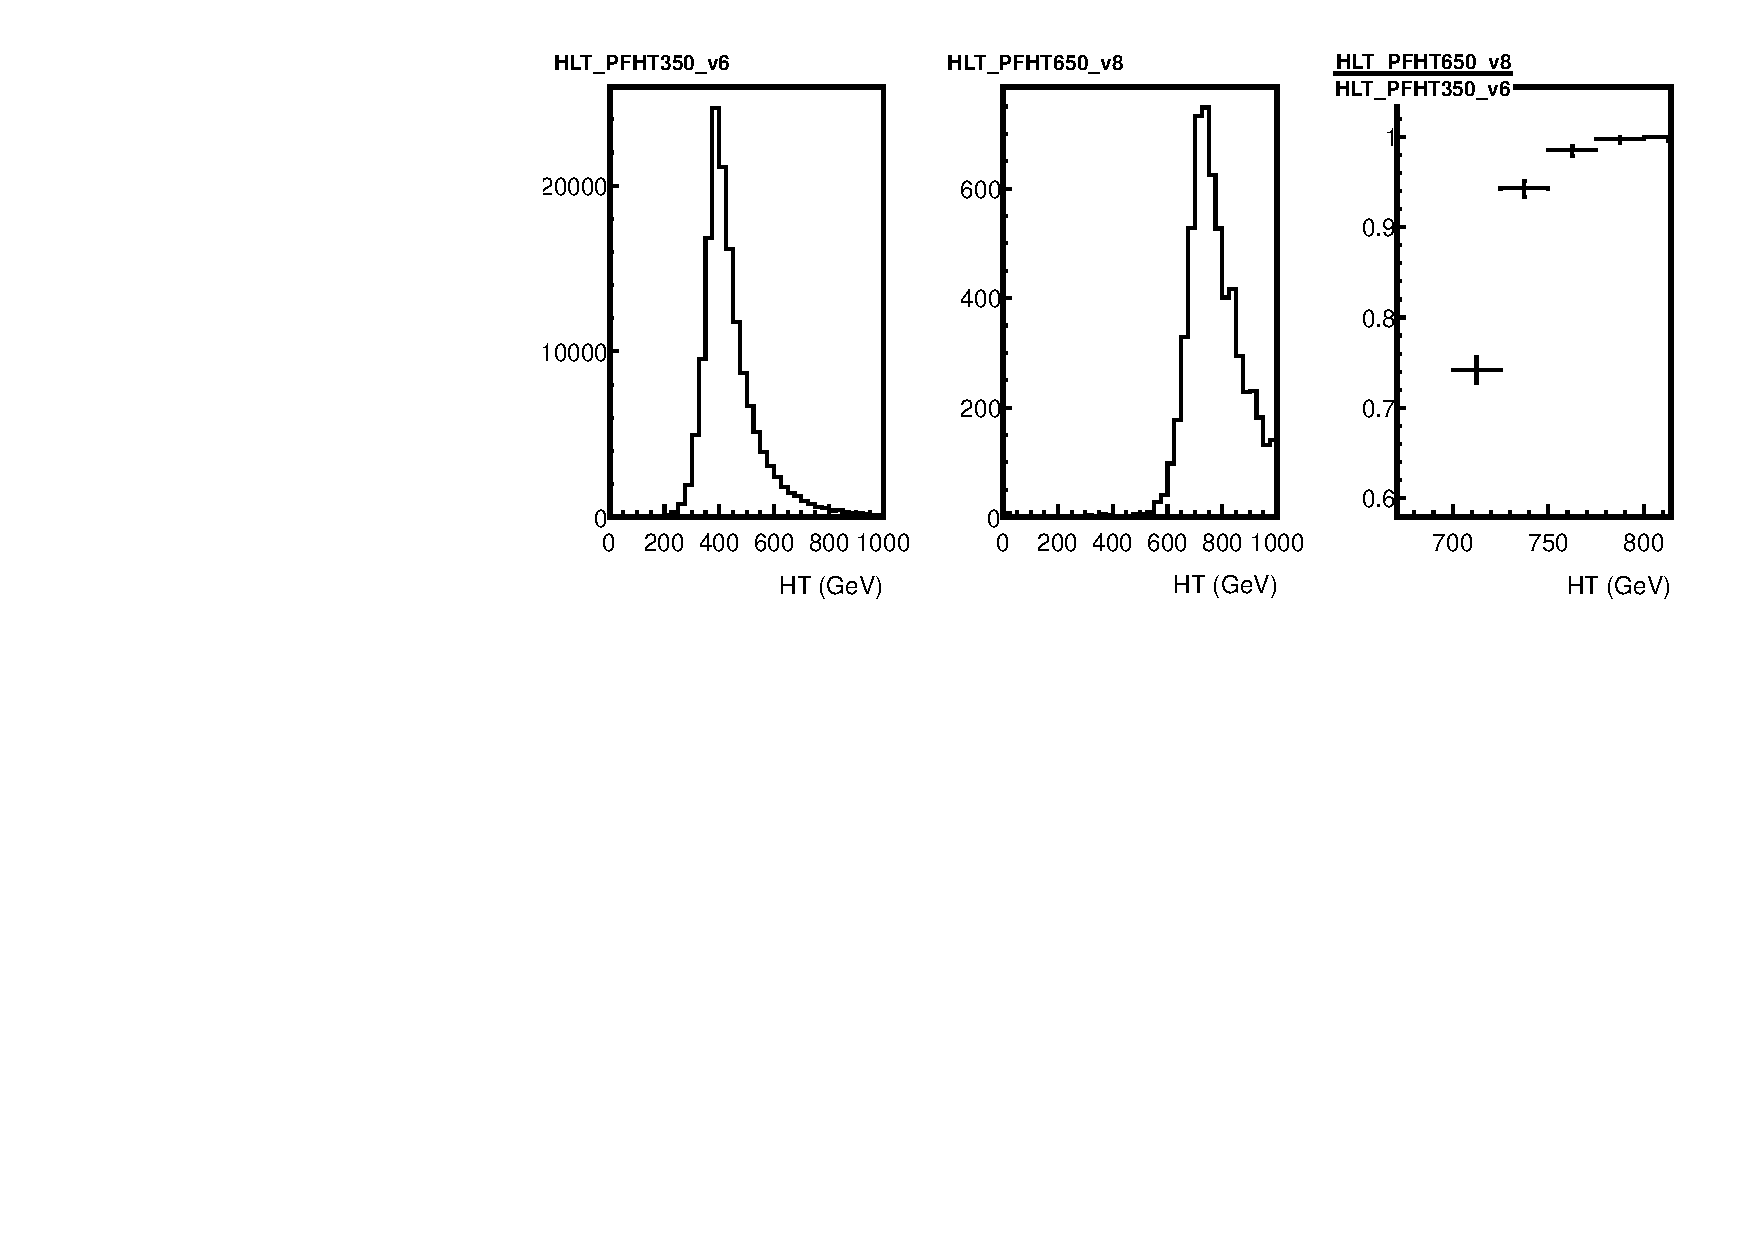
\includegraphics[width=1.0\textwidth]{figs/TriggerDemonstration.pdf}
\caption{The prescaled (left) and  un-prescaled (middle) HT triggers. The right plot shows the ratio of the two previous histograms 
zoomed in the interesting part.}
\label{fig.TriggerPlateau}
\end{figure}
we look at the efficiencies bin-by-bin and distribution of efficiencies (un-prescaled divided by the prescaled, 
figure \ref{fig.TriggerPlateau} (right)) 
with different HT cuts are weighted according to the statistics of the un-prescaled histogram. 
The cut that gives the mean value greater than 95\% is chosen as the offline cut on the trigger parameter. 
An example of this method for different cuts on the HT for HLT\_PFHT650\_vX is shown in figure \ref{fig.TriggerEff}.
\begin{figure}[!htb]
\centering
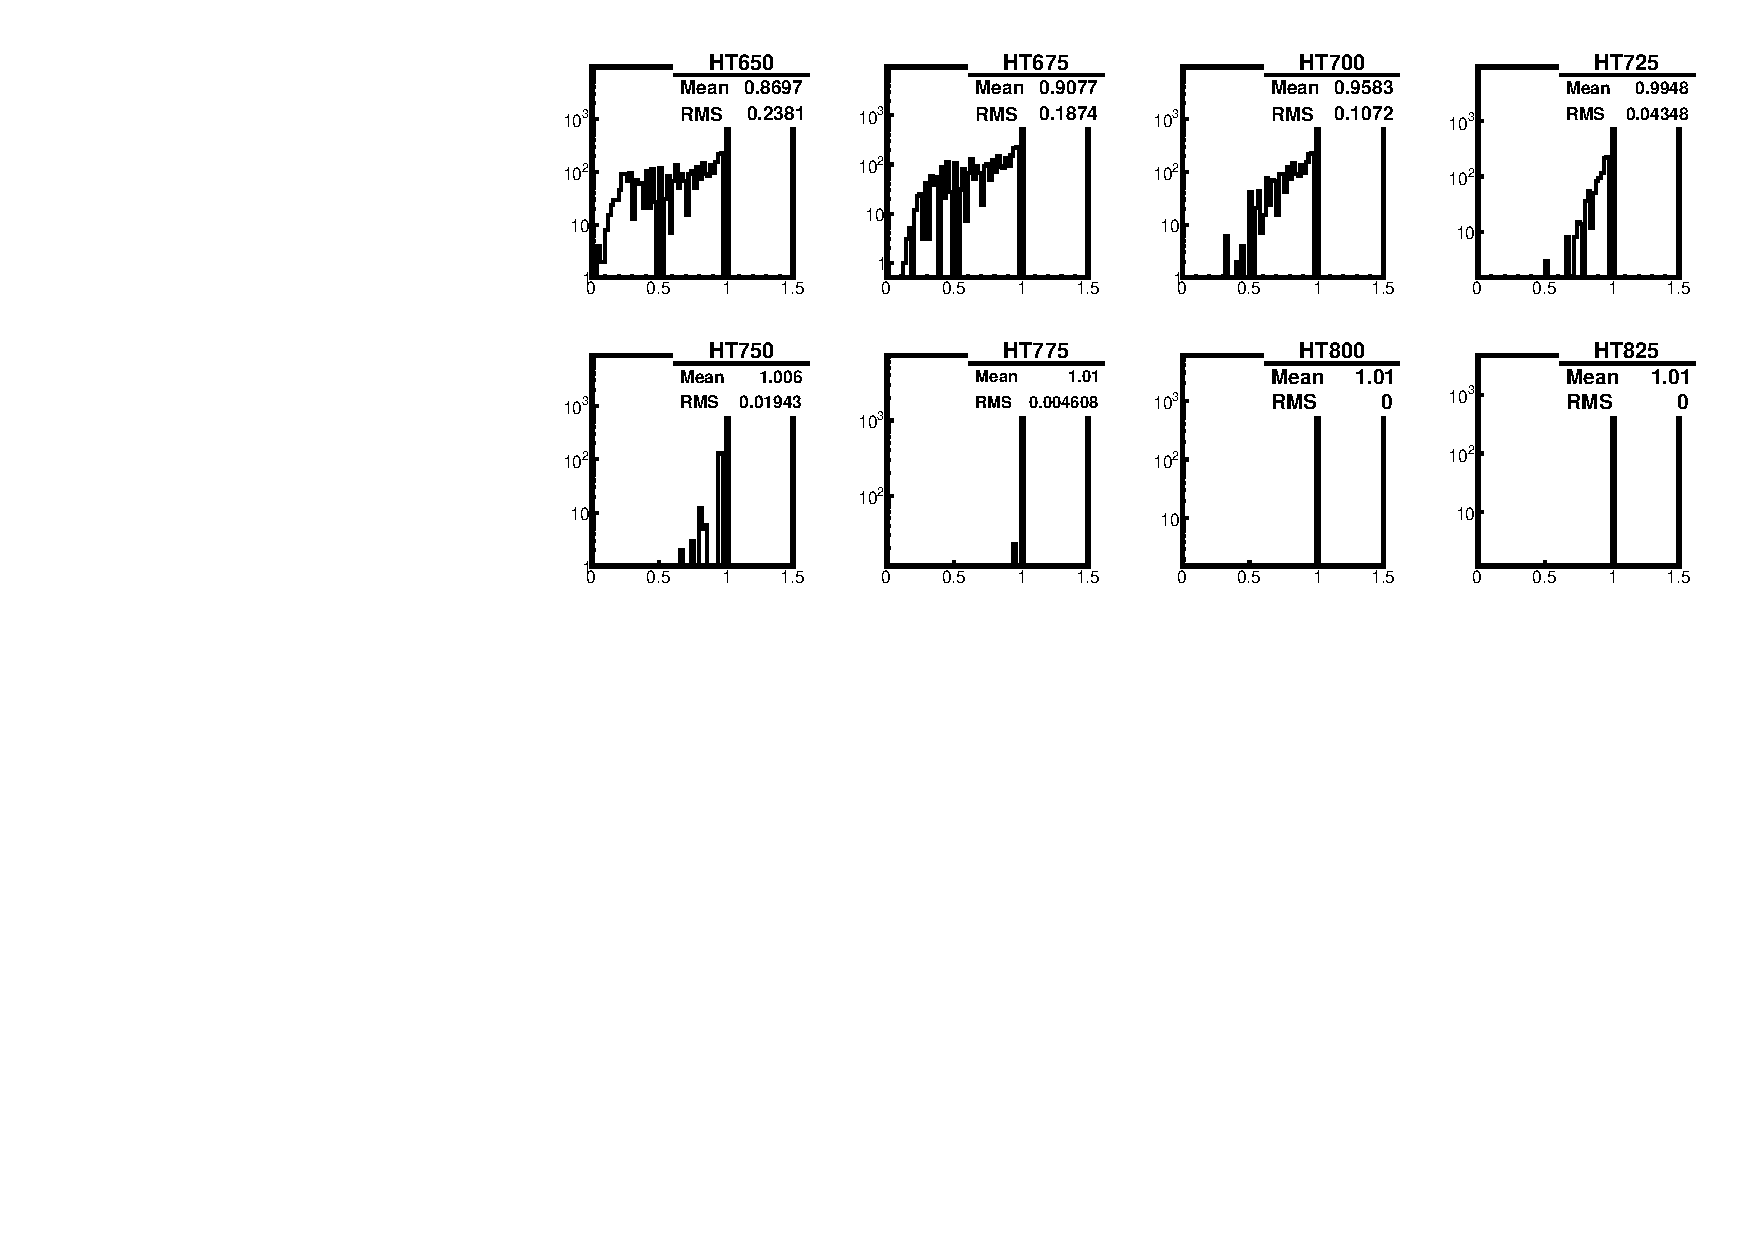
\includegraphics[width=1.0\textwidth]{figs/TriggerDemonstrationEff.pdf}
\caption{The weighted mean of the efficiencies in figure \ref{fig.TriggerPlateau}(right) for different cuts on HT. 
HT $>$ 700 GeV gives 95\% efficiency.}
\label{fig.TriggerEff}
\end{figure}

The result of this method is HT $>$ 700 GeV, but we use 725 GeV conservatively. For the multijet triggers, same method is used and 
depending on the number of jets different cuts on the  $P_T$ of the jets are found. The result is summarized here:
\begin{itemize}
\item HLT\_SixJet45\_vX, 6 jets with \pT $>$ 65 GeV/$c$ or 7 jets with \pT $>$ 55 GeV/$c$
\item HLT\_QuadJet80\_vX, 4 jets with \pT $>$ 100 GeV/$c$ or 5 jets with \pT $>$ 85 GeV/$c$
\end{itemize}
As another possibility, one can think of decreasing the number of jets and increasing the \pT threshold, but it does not reach the
plateau and is excluded from the list.
Asking for 7 jets means that we rely on ISR/FSR and it is not safe from the systematic point of view, the increase of the yield due 
to adding this cut is negligible (606 events in data increases to 615), so this part is dropped from the offline cuts. 

After increasing the statistics to \IL, the following online triggers with the same offline triggers are added to the analysis.
\begin{table}[!htb]
\begin{center}
\caption{On line triggers and run ranges. A logical OR between SixJet and QuadJet is used.}
\label{Tab.TriggerPathsCnt}
\begin{tabular}{|l|c|}
\hline
HLT\_SixJet45\_v4  & 198022 - 199608\\
HLT\_SixJet45\_v6  & 199698 - 209151\\
HLT\_QuadJet80\_v4 & 198022 - 199608\\
HLT\_QuadJet80\_v6 & 199698 - 209151\\
\hline
\end{tabular}
\end{center}
\end{table}

\subsection{Trigger Selection}
\label{sect:triggerselection}
{\bf FIXME The plots need to have similar styles.}
To investigate the efficiency of different trigger sets the SMST2tt sample is used. The selection cuts described in section \ref{subsect:mt2bcuts} are applied on top of the trigger selection. The ratio of the signal events passing all the cuts is shown for two different sets of triggers as a function of $\tilde{t}$ mass and $\tilde{\chi^0_1}$ mass in figure \ref{fig:trg_eff}. Although the signal efficiency is $\sim 4$ times larger when the $HT$ trigger is used, MC studies show that the number of remaining backgrounds are so larger that the multi-jet trigger is more powerful to exclude. The estimated exclusion power of both triggers are compared in figure \ref{fig:trgs_exclusion_powers}.

\begin{figure}[htbp] 
\centering
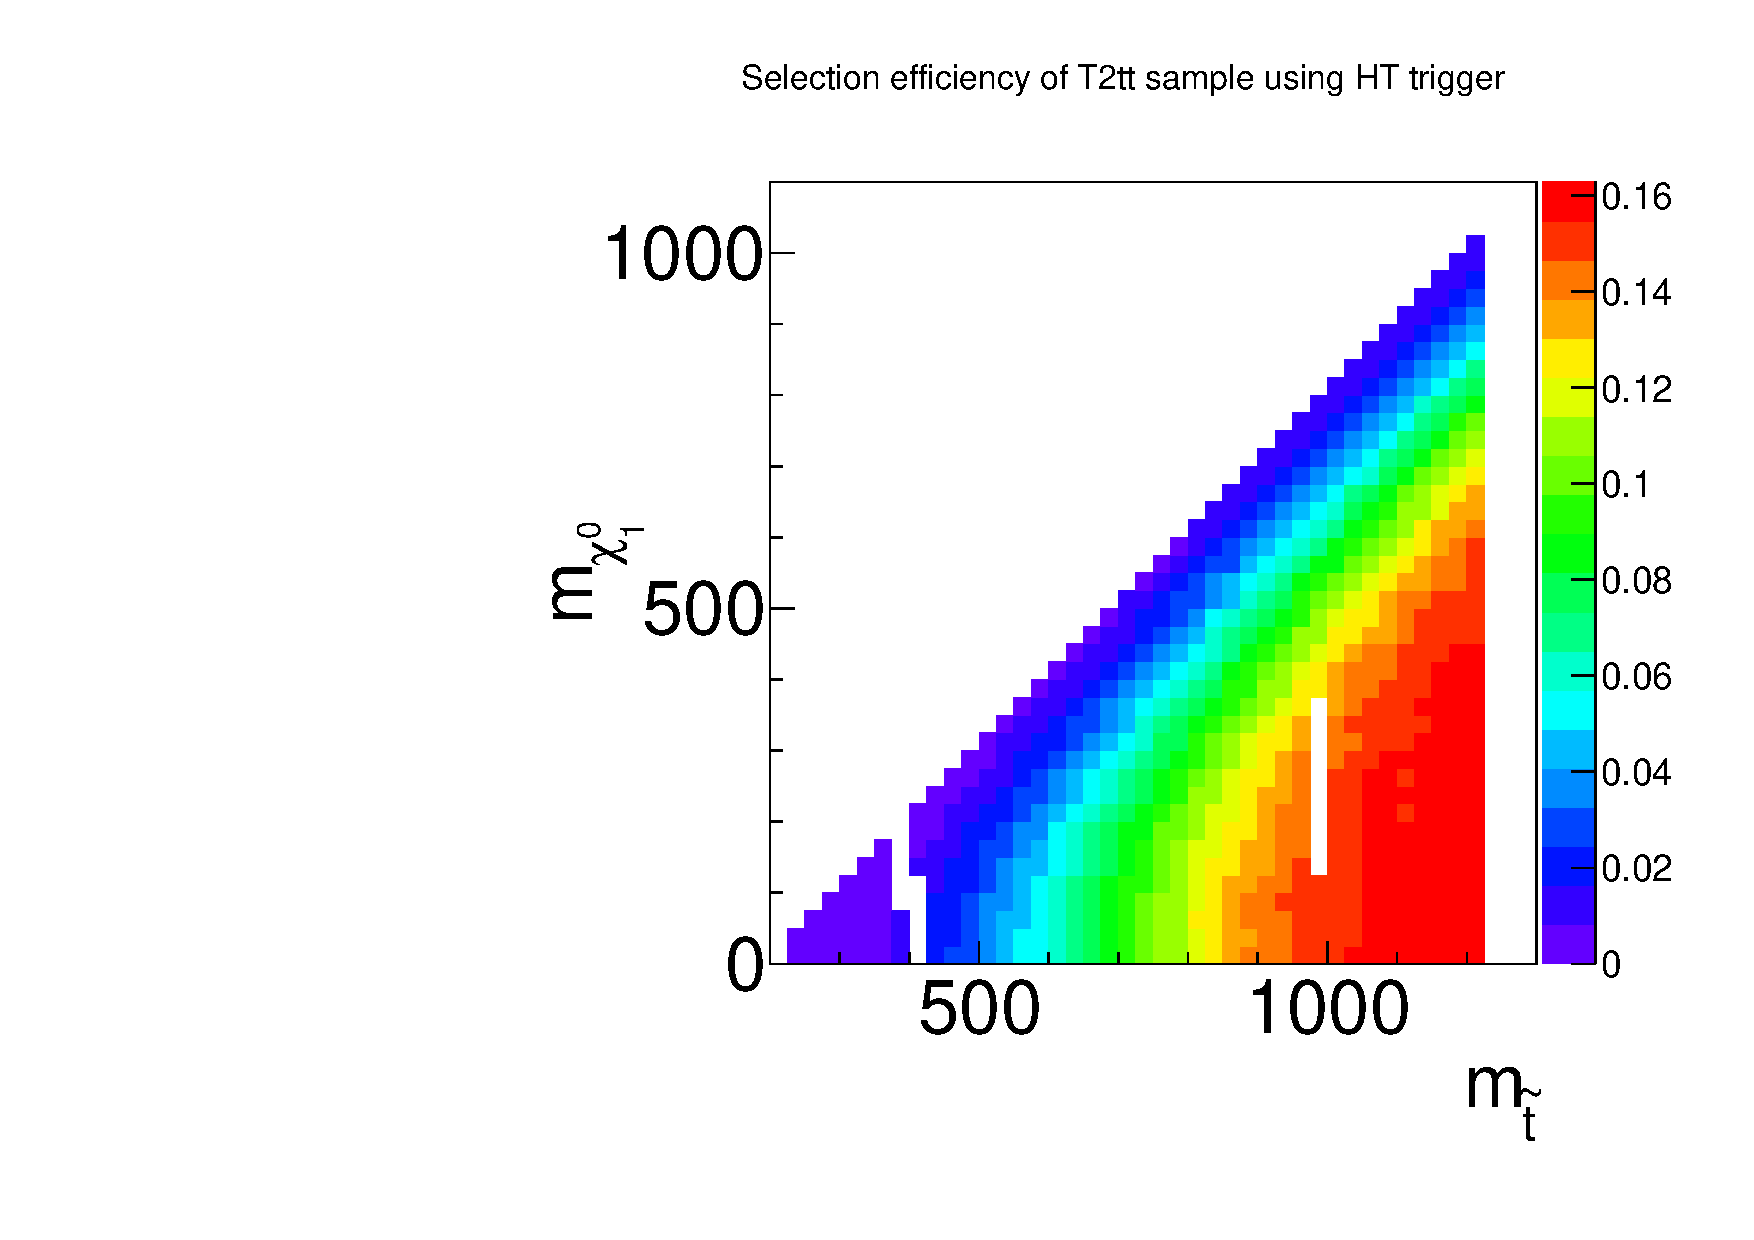
\includegraphics[angle=0,scale=0.39]{figs/HT_eff.pdf}
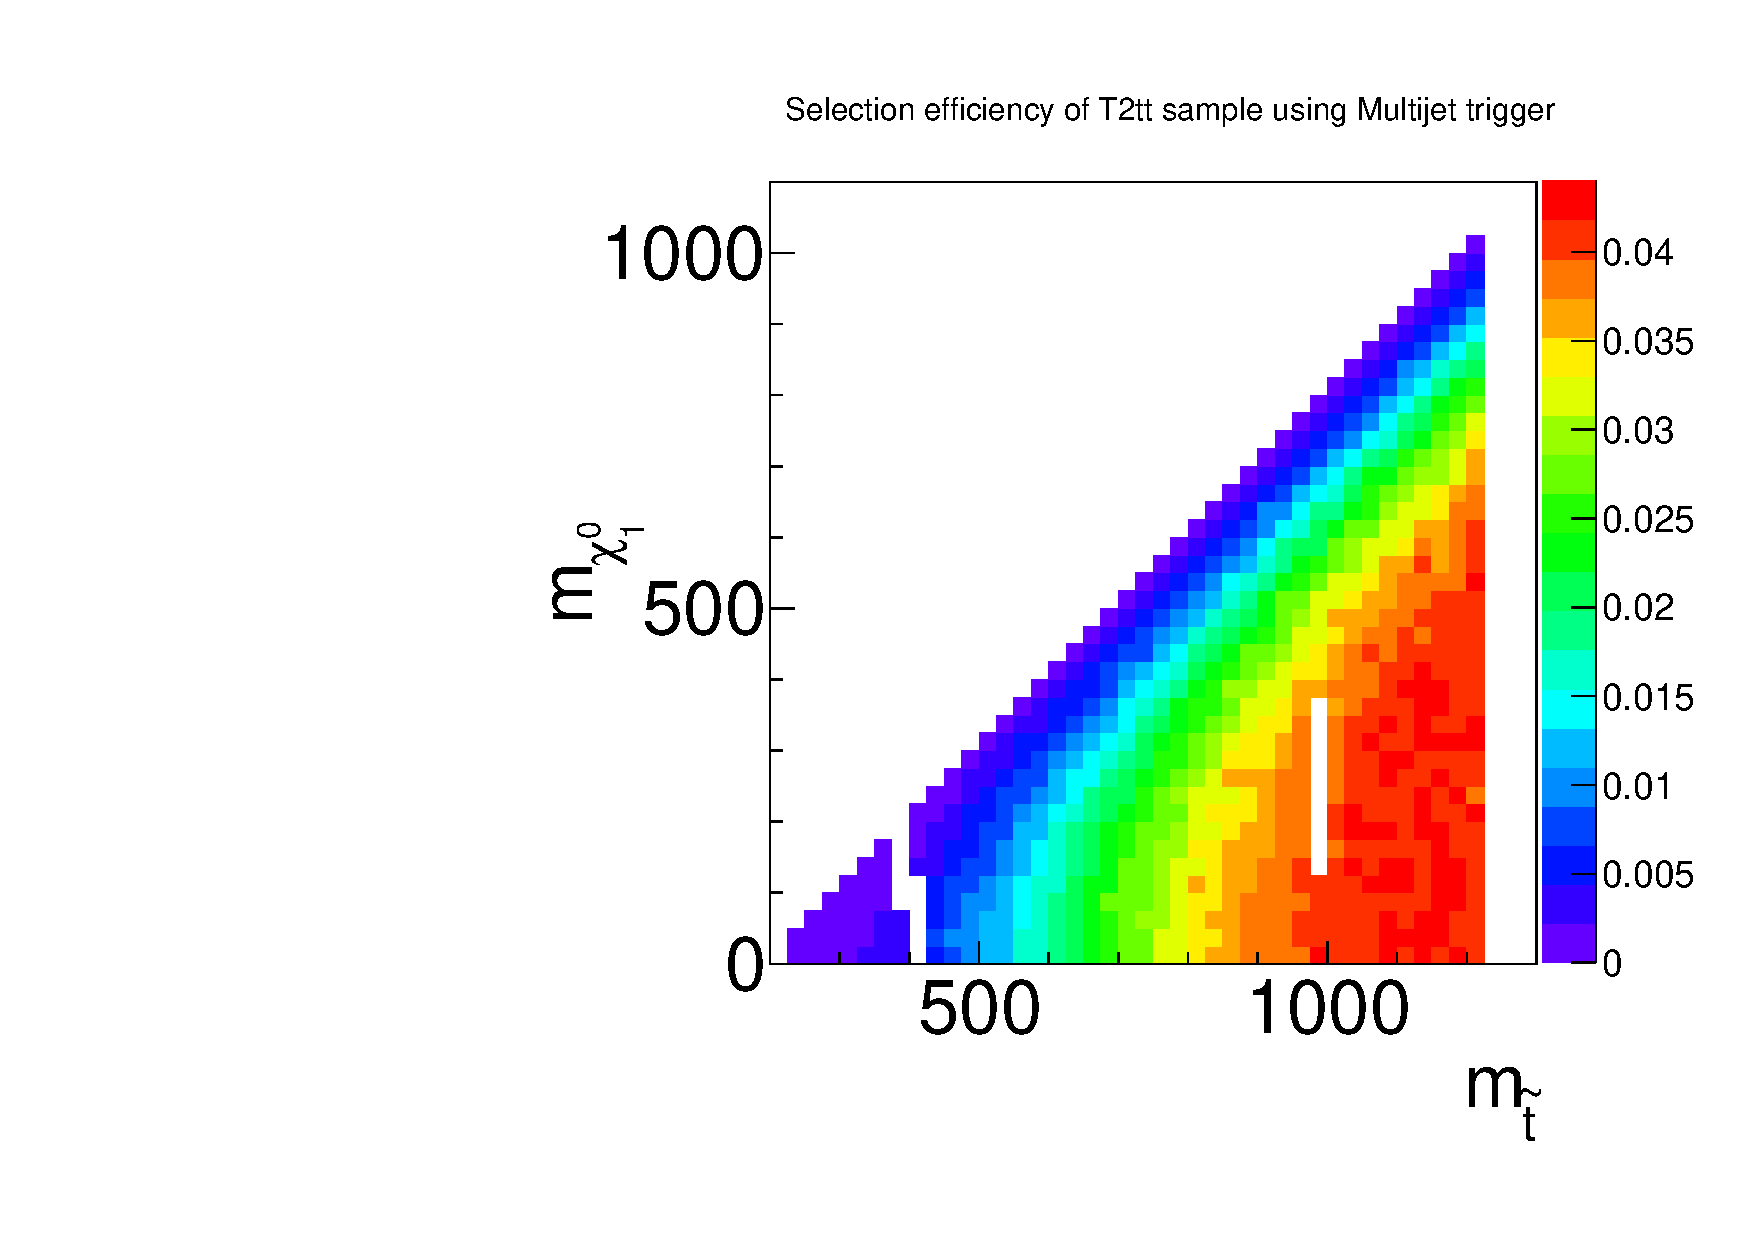
\includegraphics[angle=0,scale=0.39]{figs/multijet_eff.pdf} \\
\caption{The efficiency of different trigger sets (Left : HT trigger, Right : Multijet trigger) for the SMST2tt sample. The results are shown as a function of the $\tilde{t}$ mass and $\tilde{\chi^0_1}$ mass.}
\label{fig:trg_eff}
\end{figure}

\begin{figure}[htbp] 
\centering
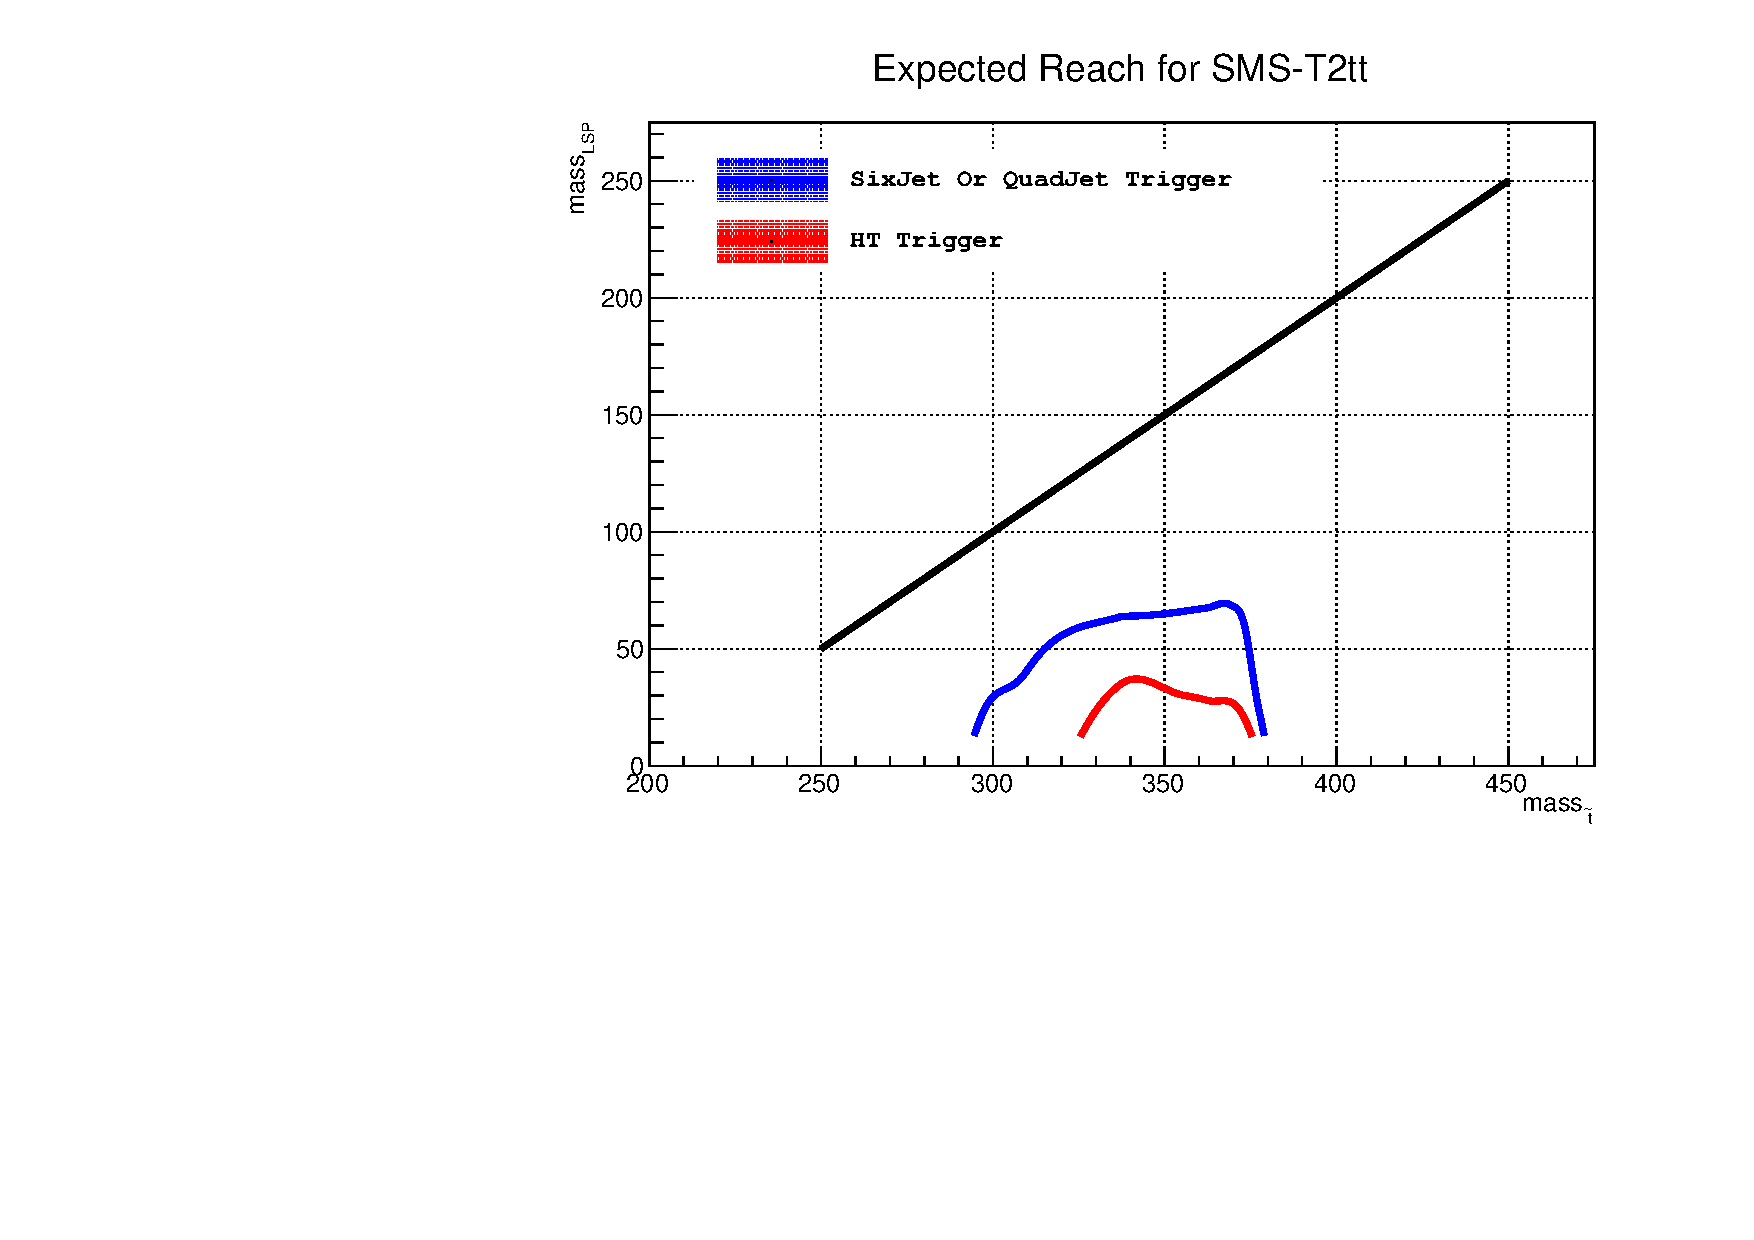
\includegraphics[angle=0,scale=0.5]{figs/SMST2tt_20121114.pdf}
\caption{The estimated exclusion power for two different sets of triggers. The multijet trigger is used in this analysis.}
\label{fig:trgs_exclusion_powers}
\end{figure}

\section{Selection Cuts}
\label{sect:cuts}

%{\bf FIXME material for the cut justification/pile up reweithing/BTg SF can appear here.}

In order to select signal events and suppres SM backgrounds, a set of cuts which are listed below, is applied.
\begin{itemize}
\item The preselection cuts which was outlined in Section~\ref{subsect:presel}.
\item Offline trigger cuts mentioned in Section ~\ref{sect:triggerstudy}. They ask for at least 4 jets with $\abs\eta<2.4$
%\item At least 4 jets with $p_T>40$ GeV and $\abs\eta<2.4$ are required which are asked to pass loose pf-jet id cuts.
\item Among these set of jets, first and second leading jets are needed to have a \pT greater than $100$ GeV and $60$ GeV, respectively.
\item It is also required that each jet with \pT $>$ 50 GeV pass loose pf-jet id cuts.
\item At least one b-quark jet is requested with \pT $>$ 20 GeV within the tracker acceptance, which is tagged by the Combined Secondary Vertex (CSV) algorithm with a tight working point.
\item The difference between \met and the vectorial \pT sum of the selected jets, electrons and muons should be below $70$ GeV.
\item The \mindphifour of the four leading jets should be greater than 0.3. There is no requirement on the id or \pT of the jets when looking for the minimum azimuthal angle between \met and jets. 
\item \met is required to be greater than $30$ GeV. 
\item Leptons, being either electrons or muons, are vetoed.
\item A cut on \mttwo $>$ 125 GeV is applied.
\end{itemize}

The effect of the selection cuts on different backgrounds is shown is Table \ref{Tab.CutFlow}

\begin{table}[!htb]
\begin{center}
\begin{tabular}{|c|c|c|c|c|c|}
\hline
% Cut                            &      QCD   &$W$+jets & $Z$+jets & Top      & Total \\\hline    %&SUSY &MJ-Data&
% Trigger                        & 5404833    & 8155.97 & 2490.53  & 62465.45 &5477944.96$\pm$24563.93\\ %SUSY 718.16   Data  4485758.00
 %Jet ID                         & 5713982.08 & 7292.60 & 2432.95  & 60040.64 &5783748.26$\pm$26645.46\\%SUSY  717.67   Data  4484247.00
 %Lepton Veto                    & 5709941.35 & 4759.89 & 1855.46  & 51143.85 &5767700.56$\pm$26642.92\\%SUSY  619.95    Data 4469115.00
 %BJet                           & 583250.20  & 323.93  &  155.37  & 34252.57 &617982.07$\pm$8690.65\\  %SUSY  447.29   Data 578345.00
 %\mindphifour$>$ 0.3            & 310092.56  & 198.38  &  103.58  & 19147.93 &329542.46$\pm$6437.28\\  %SUSY  338.33   Data 318801.00
 %$M_{T2} >$ 125                  & 465.73     & 30.99   &   22.92  & 561.55   &1081.19$\pm$121.23\\  %SUSY  150.12  Data  779.00&
%$|\met -MHT| <$ 70             &  72.22     &  27.66  &  20.47   &  470.25  &590.61$\pm$21.63\\  %SUSY  135.45  Data  606.00&
           
 Cut                  &      QCD   &$W$+jets & $Z$+jets & Top      & Total \\\hline    
Trigger               & 5404833    & 8155.97 & 2490.53  & 62465.45 & 5477944.96$\pm$24563.93\\
Jet Id                & 5398500.97 & 8155.97 & 2490.53  & 62458.38 & 5471605.85$\pm$24530.03\\
Lepton Veto           & 5395465.53 & 5328.26 & 1950.00  & 53172.66 & 5455916.45$\pm$24529.43\\
BJet                  & 548011.88  & 361.80  & 163.32   & 35523.88 & 584060.88$\pm$10321.31\\
\mindphifour$>$ 0.3   & 297576.19  & 221.37  & 109.44   & 19851.70 & 317758.70$\pm$8400.29\\
$|\met -MHT| <$ 70    & 253056.18  & 192.73  & 98.83    & 16860.00 & 270207.73$\pm$8276.51\\
$M_{T2} >$ 125        & 113.19     & 30.87   & 22.74    & 500.33   & 667.14$\pm$28.28\\

\hline
\end{tabular}
\caption{Event yields after applying different cuts. "Trigger" contains all of the preselections and offline trigger cuts.}
\label{Tab.CutFlow}
\end{center}
\end{table}


\section{Search Strategy}
\label{sect:search}
The \mttwo distribution in Figure \ref{fig:MT2}
\begin{figure}[!htb]
\centering
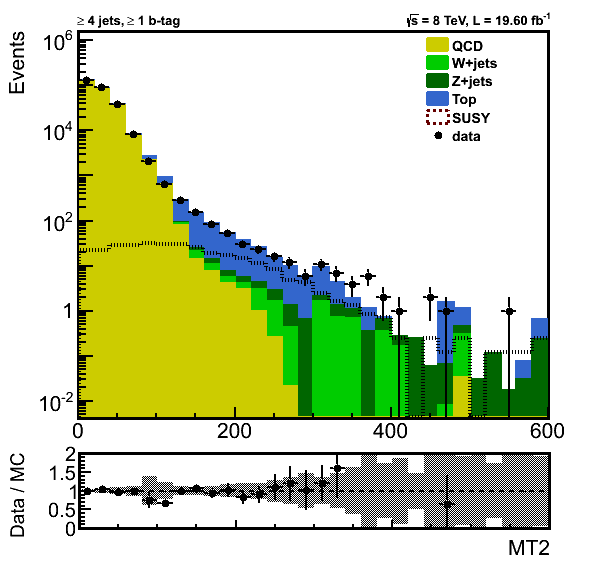
\includegraphics[width=0.49\textwidth]{figs/MT2SmearedJetMET.png}
\caption{\mttwo distribution after applying the full selection cuts.}
\label{fig:MT2}
\end{figure}
is used as a variable to search for SUSY. With comparing the data and MC in the QCD dominated region (\mttwo $<$ 60 GeV), 
a flat scale factor of 1.474 is found for the QCD samples to have a good agreement between data and MC.
To increase the power of the analysis, a multibinning approach is used.
We select 4 bins in \mttwo with the edges of 125, 150, 200, 250 and infinity.
Every \mttwo bin is devided to two bins with number of the reconstructed top quarks equal to or greater than 0.
This leads to 8 bins in total. In this round of analysis, we try to emphasize the complementary role of this anaysis
for the common cut and count hadronic search for the direct stop production. Since this analysis does not use the \met explicitly, it is more sensetive to the small mass differences between stop and LSP.
\section{Backgrounds}
\label{sect:bkg}
In this section, data driven methods are proposed and applied to estimate the contribution of the main background processes. 
Most of the methods are similar to what were used in the \mttwo analysis \cite{MT2_2011} with some minor changes which are explained
here.


\subsection[QCD Estimation]{Data-driven background estimation of QCD}\label{subsect:qcd}

Due to inadequate statistics of QCD Monte-Carlo samples and complicated nature of this background, 
we use a data driven method to estimate its rate in the tail of the $\mttwo$ distribution, while the simulation shows that it is small.

We follow the method, fully discussed and applied by the $\mttwo$ and $M_{T2b}$ groups \cite{MT2_2011},
 but the parameters are finely tuned to the conditions of our analysis.
The method indeed relies on different distributions of QCD and SUSY-like events 
in the plane of $\mttwo$ and $\mindphifour$, 
the azimuth-difference between the $\met$ vector and the closest selected jet.

%%%%%%%%%%
\begin{linenomath}
\begin{figure}[h]
\centering
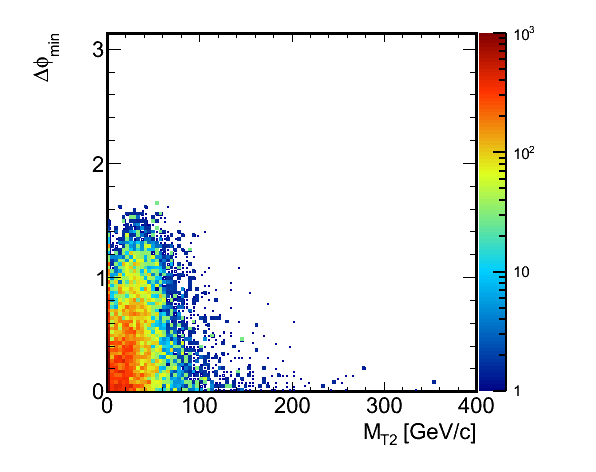
\includegraphics[width=0.49\textwidth,keepaspectratio=true]{QCDFig/qcd_distribution.png}
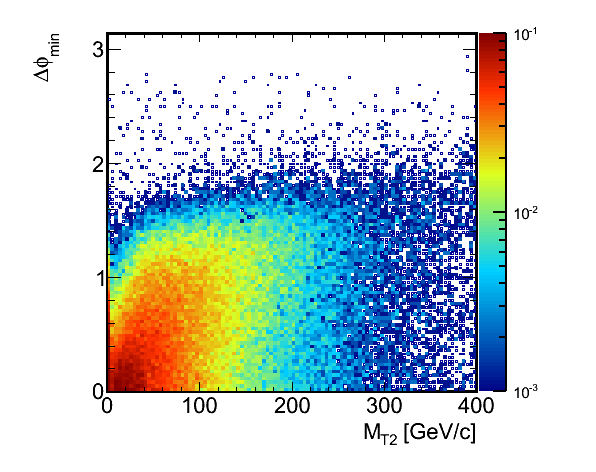
\includegraphics[width=0.49\textwidth,keepaspectratio=true]{QCDFig/sms_distribution.png}
\caption[DPhi vs. MT2 Distribution]{Distribution of $\mindphifour$ versus $\mttwo$ for (left) QCD and 
(right) SUSY-like (SMS) simulated events. QCD events are populated in the low $\mindphifour$ and $\mttwo$ region, while
SUSY events spread over the plane.}
\label{fig:distributions}
\end{figure}
\end{linenomath}
%%%%%%%%%%

Figure \ref{fig:distributions} shows such distributions for QCD (left) and SMS samples (right).
Unlike the broad spread of SMS events in this plane, QCD events are densely populated 
in the low $\mindphifour$ and $\mttwo$ region.
Due to the strong correlation between the two variables of $\mindphifour$ and $\mttwo$, 
the usual ABCD method is inefficient, whereas a factorization method \cite{MT2_2011} is still applicable.
The method works based on the ratio of $r(\mttwo) = N (\mindphifour \geq 0.3)/N (\mindphifour \leq 0.2)$ 
as a function of $\mttwo$ for QCD events. Figure \ref{fig:qcd_ratio} shows the ratio $r(\mttwo)$ in the QCD simulation. 
It indicates an exponentially descending behavior
%  of the ratio $r(\mttwo)$ for the QCD simulation on 
in the region of $\mttwo > 50$ GeV (the lower bins of $\mttwo$ could be biased by the minimal cut on $\met$). 
Hence, we characterize such specification of the QCD events by the model 
of 
%%%%%%%%%%  
\begin{align}\label{eq:rmt2}
 r(\mttwo) = \frac{N(\mindphifour \geq 0.3)}{N(\mindphifour \leq 0.2)} = e^{a-b.\mttwo}+c
\end{align}
%%%%%%%%%%

% where the parameters of $b$ and $a$ indicate slope-intercept form of the straight line
where a and b parameters indicate respectively the slope and the intercept of the straight line
 in the logarithmic scale. 
Ratio $r(\mttwo)$
%Function \ref{eq:rmt2} 
tends towards 
% the constant value of c at the large value of $\mttwo$.
constant value, c, at large values of $\mttwo$.
The red curve in Figure \ref{fig:qcd_ratio} shows the fit of model (Equation \ref{eq:rmt2}) to the QCD simulation and 
Table \ref{tab:qcd_fit} presents the value of parameters as a result of the fit in the range of $\mttwo > 60$ GeV (the first column). 

%%%%%%%%%%
\begin{linenomath}
\begin{table}[h]
\begin{center}
\small
\begin{tabular}{l|cc}\hline\hline

Parameter & $\mttwo > 60$ GeV & $60 < \mttwo < 80$ GeV \\ \hline
a & $2.07\pm0.14$ & $2.22\pm0.46$ \\
b (GeV$^{-1}$) & $0.0226\pm0.0019$ & $0.0245\pm0.0062$ \\
c & $0.0504\pm0.0039$ & - \\ \hline\hline
%a & $2.78\pm0.17$ & $2.94\pm0.41$ \\
%b (GeV$^{-1}$) & $0.0320\pm0.0021$ & $0.0325\pm0.0058$ \\
%c & $0.0139\pm0.0076$ & - \\ \hline\hline
\end{tabular}
\caption[Fit results for QCD]{The result of the two different parametrizations for ratio $r(\mttwo)$ in QCD simulated events.}  
\label{tab:qcd_fit}
\end{center}
\end{table}
\end{linenomath}
%%%%%%%%%%

In real data, to have a pure QCD sample with the minimal contamination from non-QCD backgrounds, we have to 
concentrate on the region of low $\mttwo$ ($60 < \mttwo < 80$ GeV). 
The fit of ratio $r(\mttwo)$ on this short range of $\mttwo$ can be reasonably described as a straight line in the logarithmic scale.
Thus, it is not able to give parameter c. 
The green curve in Figure \ref{fig:qcd_ratio} shows the linear fit and 
the second column of Table \ref{tab:qcd_fit} presents the relevant parameters, a and b.
As 
seen 
%taken 
from Figure \ref{fig:qcd_ratio}, both fits (green and red) are in 
a very good agreement at low $\mttwo$, while the second fit (the green straight line), 
called optimistic parameterization, gives the lower values for ratio $r(\mttwo)$ 
at high $\mttwo$. 
Hence, a realistic model needs also the parameter c to parameterize 
the ratio $r(\mttwo)$ in the entire range of $\mttwo$. 
% To solve the arisen problem 
we conservatively 
% chose to 
take the parameter c from the straight line at $\mttwo = 200$ GeV. 
The blue curve of Figure \ref{fig:qcd_ratio} represents such a fit, 
namely pessimistic parameterization. 

%%%%%%%%%%
\begin{linenomath}
\begin{figure}[h]
\centering
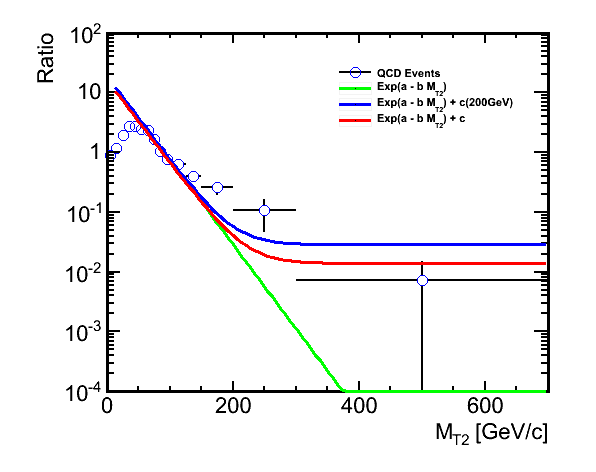
\includegraphics[width=0.7\textwidth,keepaspectratio=true]{QCDFig/qcd_ratio.png}
\caption{Three different fits of ratio $r(\mttwo)$  in QCD simulated events. 
The red curve is an exponential function plus a constant. It uses
the entire range of $\mttwo > 60$ GeV for parametrization (fully-MC) of ratio $r(\mttwo)$. 
The green curve is just an exponential function and uses the range of $60 < \mttwo < 80$ GeV 
for parameterization (optimistic). 
The blue curve is also an exponential function plus a constant, 
however it uses the range of $60 < \mttwo < 80$ GeV for parameterization (pessimistic).}
\label{fig:qcd_ratio}
\end{figure}
\end{linenomath}
%%%%%%%%%%

Figure \ref{fig:data_ratio} depicts both parameterizations 
(optimistic and pessimistic by green and blue curves respectively) 
as a consequence of employing the method in the cleaned data.
The non-QCD contaminations, taken from the Monte-Carlo simulation, are subtracted from 
data before calculating the parameters.
Table \ref{tab:data_fit} presents the parameters a and b extracted from the fit. 
These data-driven parameters eventually fulfill the functional form of ratio $r(M_{MT2})$.

%%%%%%%%%%
\begin{linenomath}
\begin{figure}[h]
\centering
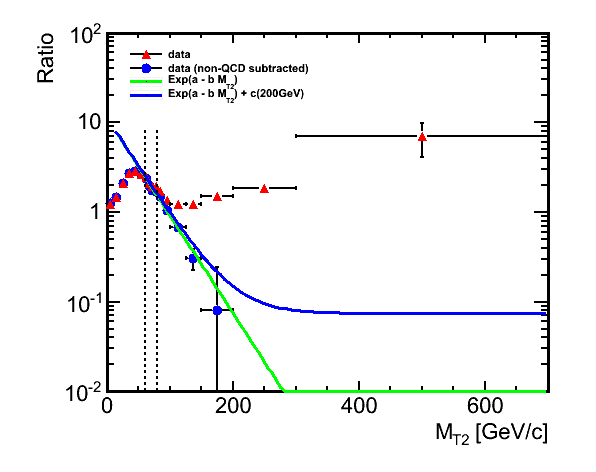
\includegraphics[width=0.49\textwidth,keepaspectratio=true]{QCDFig/data_ratio.png}
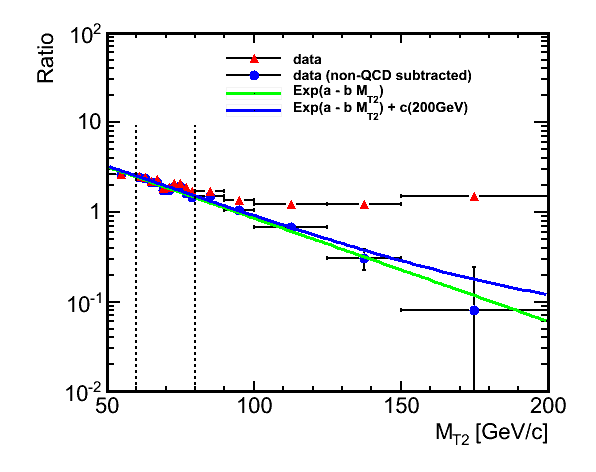
\includegraphics[width=0.49\textwidth,keepaspectratio=true]{QCDFig/data_ratio_zoom.png}
\caption{Fits of ratio $r(\mttwo)$ in the non-QCD subtracted data. 
The green and blue curves are related to optimistic
and pessimistic parameterization respectively. The right plot is a focus on the desired range of $\mttwo$ for the parametrizations.} 
\label{fig:data_ratio}
\end{figure}
\end{linenomath}
%%%%%%%%%%


%%%%%%%%%%
\begin{linenomath}
\begin{table}[h]
\begin{center}
\small
\begin{tabular}{l|c}\hline\hline
Parameter & $60 < \mttwo < 80$ GeV \\ \hline
a	&	$2.39\pm0.20$	\\
b (GeV$^{-1}$)	&	$0.0247\pm0.003$	\\ \hline\hline

%a	&	$2.41\pm0.21$	\\
%b (GeV$^{-1}$)	&	$0.0250\pm0.0031$	\\ \hline\hline

\end{tabular}
\caption[Fit results for data]{The parametrization results for ratio $\rm{r(\mttwo)}$ 
in real data (non-QCD events are subtracted, using simulation).}
\label{tab:data_fit}
\end{center}
\end{table}
\end{linenomath}
%%%%%%%%%%

In the last step of procedure, we apply the ratio $r(\mttwo)$ 
to the observed cleaned data in the QCD control region (high $\mttwo$, 
low $\mindphifour$) to estimate the number of QCD events in the signal region 
(high $\mttwo$, high $\mindphifour$). Figure \ref{fig:exp_distribution} shows 
the $\mttwo$ distribution of QCD truth observed events and 
the expected distribution from data (non-QCD subtracted). 
Furthermore, Table \ref{tab:exp_distribution} compares
the estimated with observed QCD events for several bins of $\mttwo$.
%%%%%%
In addition to the statistical uncertainties, the predicted numbers incorporate the systematic ones, coming from
the fit range. Indeed, the standard deviation of a $10\%$ fluctuation at the boundaries of the fit range, $(60 < \mttwo < 80)$ GeV, 
induces the systematic uncertainties reported in Table \ref{tab:exp_distribution}. 
%%%%%%
Considering the uncertainties, the method prediction is in good agreement with the QCD truth. 
 
%%%%%%%%%%
\begin{linenomath}
\begin{figure}
\centering
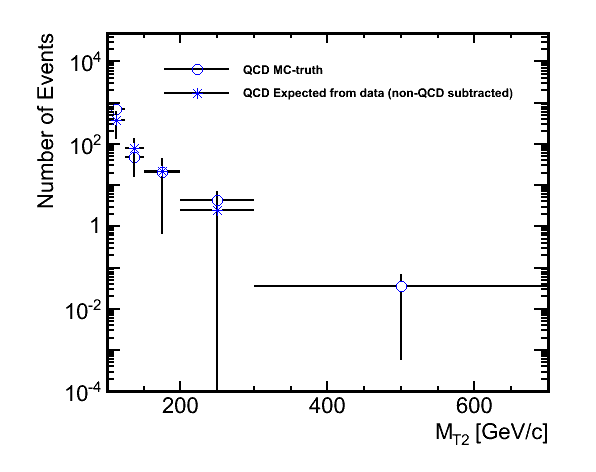
\includegraphics[width=0.7\textwidth,keepaspectratio=true]{QCDFig/exp_distribution.png}
\caption{QCD MC-truth and data-driven prediction for the distribution of $\mttwo$.}
\label{fig:exp_distribution}
\end{figure}
\end{linenomath}
%%%%%%%%%%

%%%%%%%%%%
\begin{linenomath}
\begin{table}[h]
\begin{center}
\small
\begin{tabular}{l|cc}\hline\hline
$\mttwo$ bins & MC-truth & Data-prediction \\ \hline
$[125, 150)$	&	$102.8\pm23.22$		& $80.67\pm63.56$ \\
$[150, 200)$	&	$19.12\pm2.97$		& $23.57\pm22.43$ \\
$[200, 300)$	&	$3.34\pm1.24$		& $2.59\pm3.22$ \\
$[300, \infty)$	&	$0.00\pm0.00$	& $0.00\pm0.21$ \\ \hline\hline

%$[125, 150)$	&	$48.1\pm9.1$		& $78\pm62\pm95$ \\
%$[150, 200)$	&	$20.7\pm6.0$		& $22\pm22\pm60$ \\
%$[200, 300)$	&	$4.5\pm2.6$		& $2.4\pm3.1\pm15.2$ \\
%$[300, \infty)$	&	$0.035\pm0.034$	& $0.00\pm0.21\pm0.00$ \\ \hline\hline


\end{tabular}
\caption{QCD MC-truth and data-driven prediction for the several bins of $\mttwo$.}
\label{tab:exp_distribution}
\end{center}
\end{table}
\end{linenomath}
Data-driven estimation is consistent with MC truth within the uncertainties.
%%%%%%%%%%
%       >> [125-150)    102.8 +- 23.22  80.67 +- 63.56
%        >> [150-200)    19.12 +- 2.97   23.57 +- 22.43
%        >> [200-300)    3.343 +- 1.242  2.592 +- 3.224
%        >> [300-700)    0 +- 0  0 +- 0.2165







\newpage
\subsection{Data-Driven Estimation of Lost Lepton from W+jets and Top}
\label{sect:intro}
After applying the selection cuts, described in detail in Section~\ref{sect:cuts}, the background 
events are dominated by $t\bar t$ events. Among all decay channels of top pair system, 
it is mainly the semi-leptonic decay which contributes to the background. 
This can be understood because genuine neutrino is produced in the semi-leptonic decay of 
top pair system, $t\bar t\rightarrow W^+bW^-\bar b\rightarrow b\bar bl\nu_ljj$, 
which can pass the $M_{T2}$ cut while the full-hadronic decay products, $t\bar t\rightarrow W^+bW^-\bar b\rightarrow b\bar bjjjj$, do not contain any neutrino.
This section describes a method to estimate the backgrounds from the leptonic decay of $W$ bosons, 
either from prompt production in $W+$jets events or from $W$ bosons produced in single top and 
top pair events, shown as $t(\bar t)$ for simplicity. The lepton is considered to be electron or muon.\\
Although the leptons are vetoed in the main analysis, there are still some background 
from $W\rightarrow l\nu_l$, referred to as lost lepton background events, 
contributing to the full-hadronic analysis. This is due to the acceptance cuts or 
inefficiencies in the lepton isolation and identification criteria.\\
In order to estimate the backgrounds due to the lost lepton events, all selection cuts are applied except
 lepton veto which is inverted. The distribution of the $p_T$ of the leptons in the events 
with exactly one lepton, being either electron or muon, are shown in 
Figure~\ref{fig:pt}, where it can be seen that the number of MC events are greater than the 
observed number of data events.\\
\begin{figure}[htbp] 
\centering
%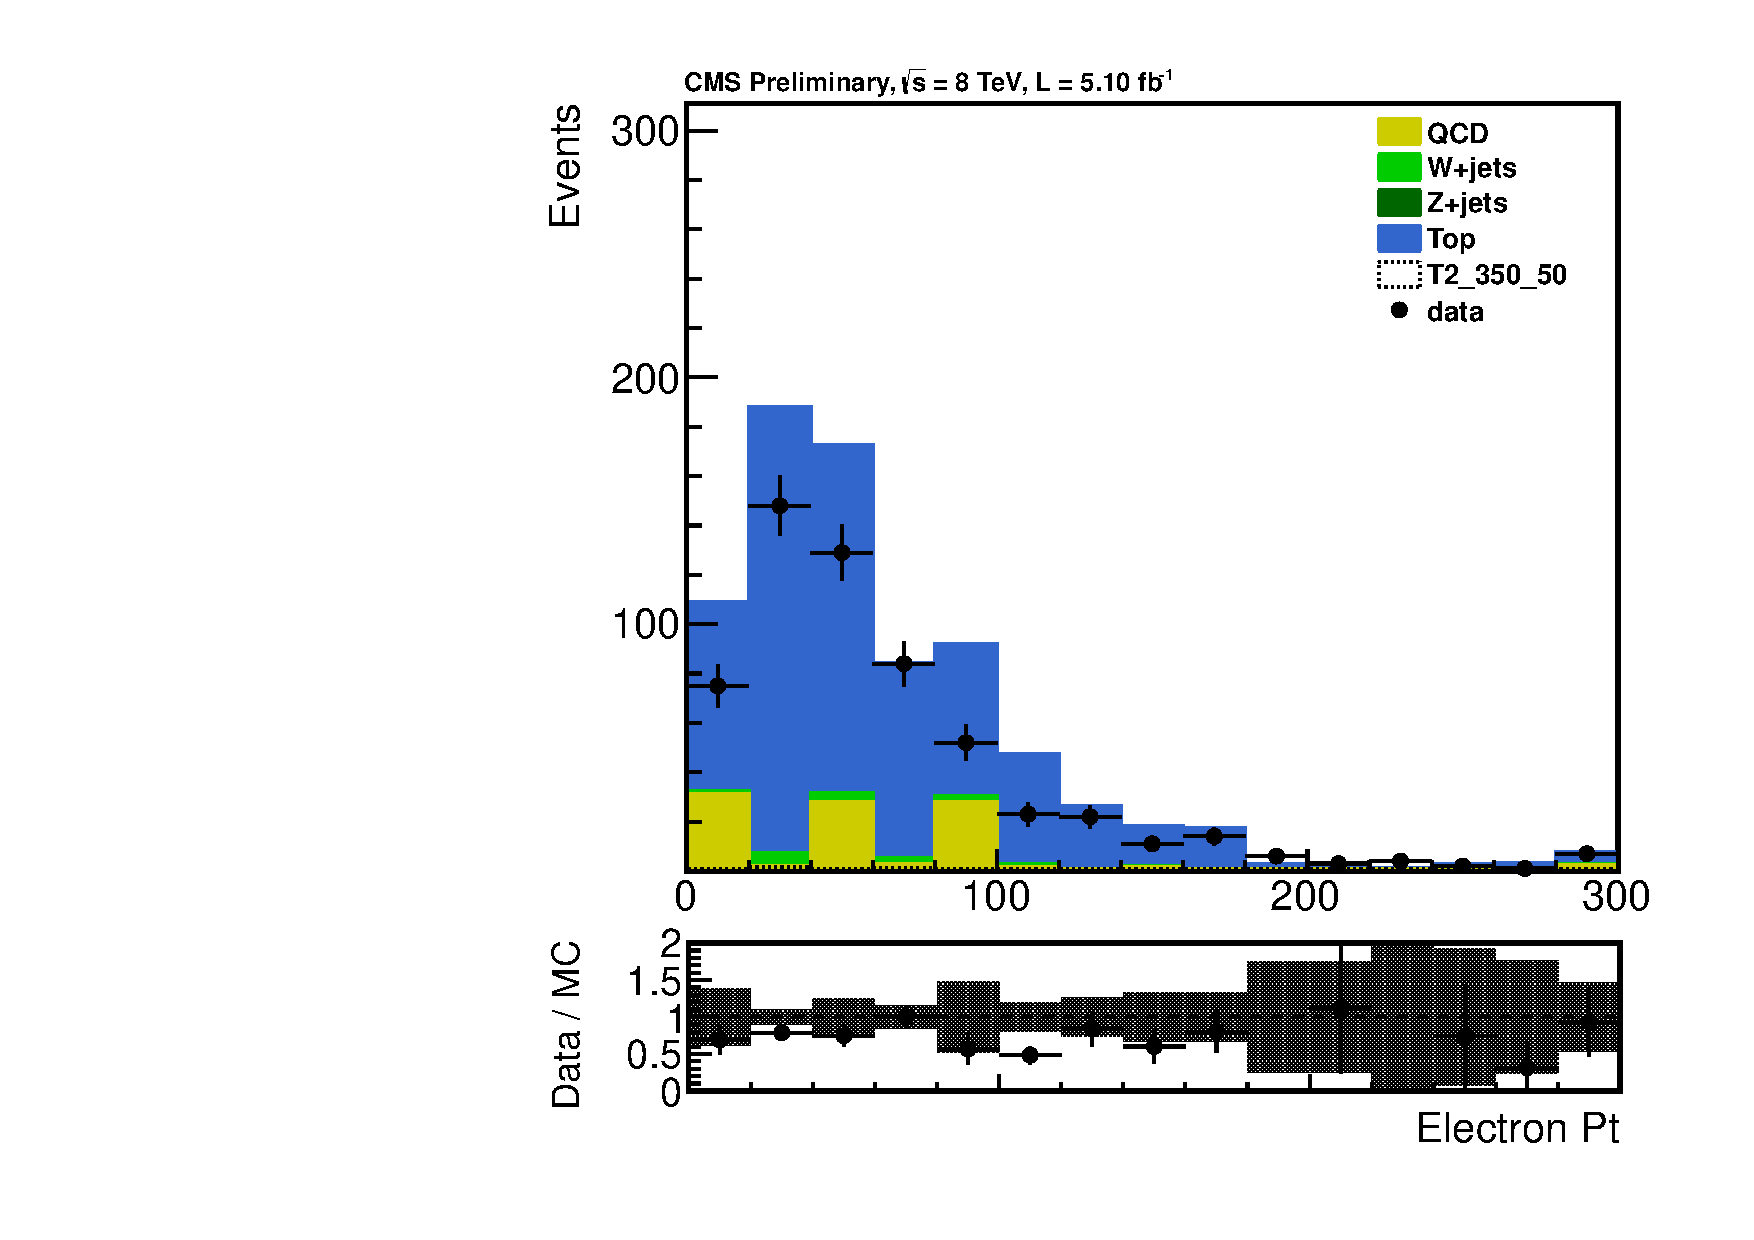
\includegraphics[angle=0,scale=0.39]{myplots/ele_pt.pdf}
%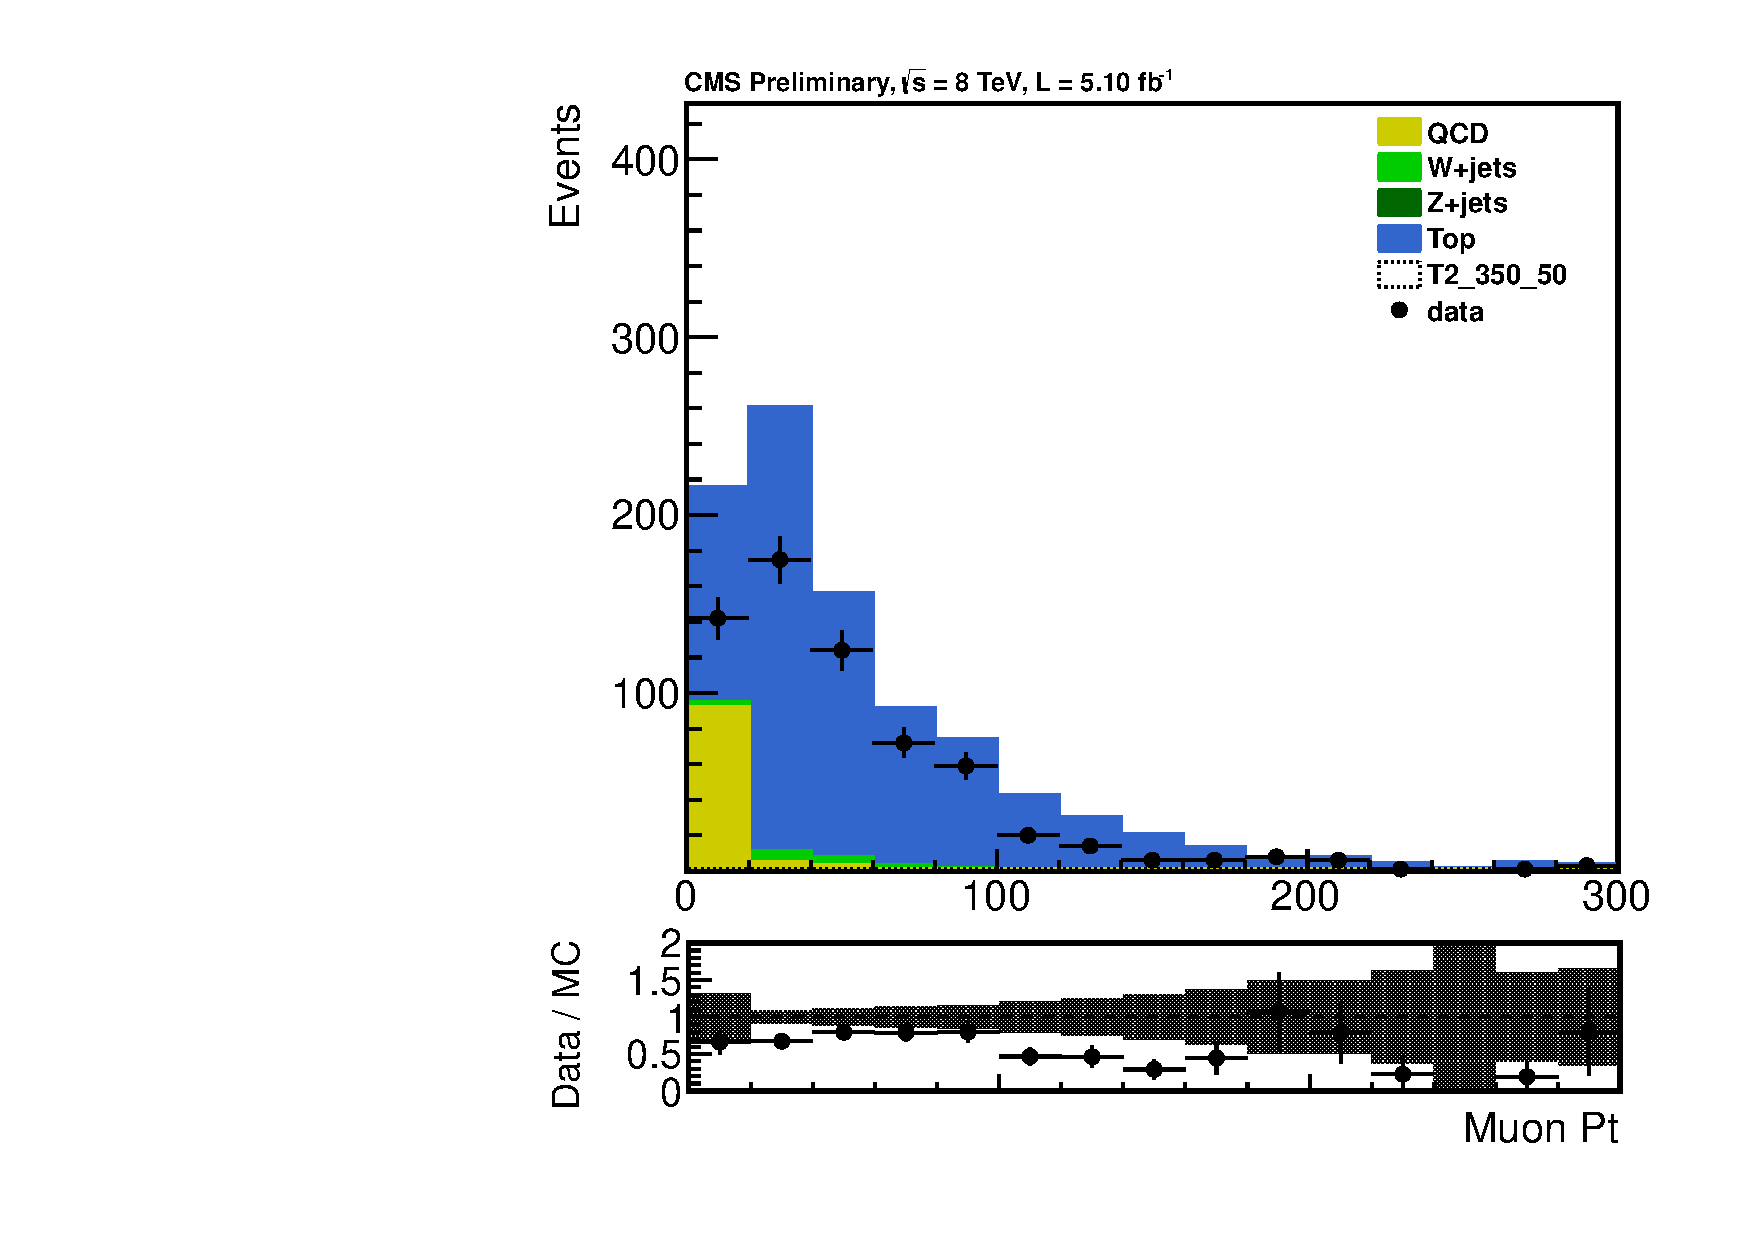
\includegraphics[angle=0,scale=0.39]{myplots/muo_pt.pdf} \\
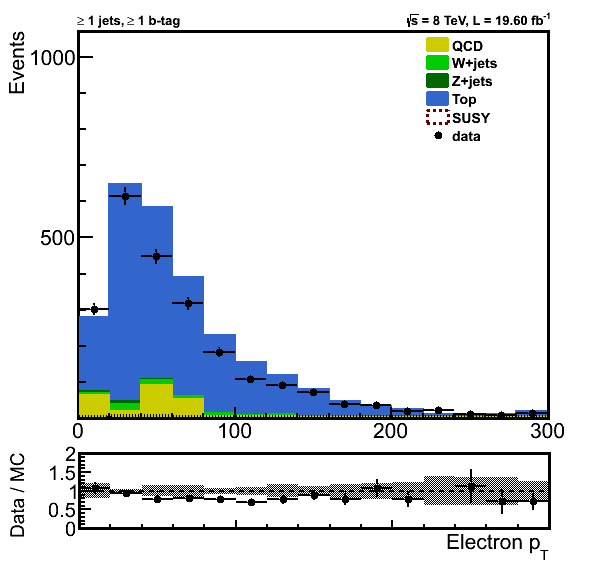
\includegraphics[angle=0,scale=0.35]{llplots_20Invfb/ele_pt.png}
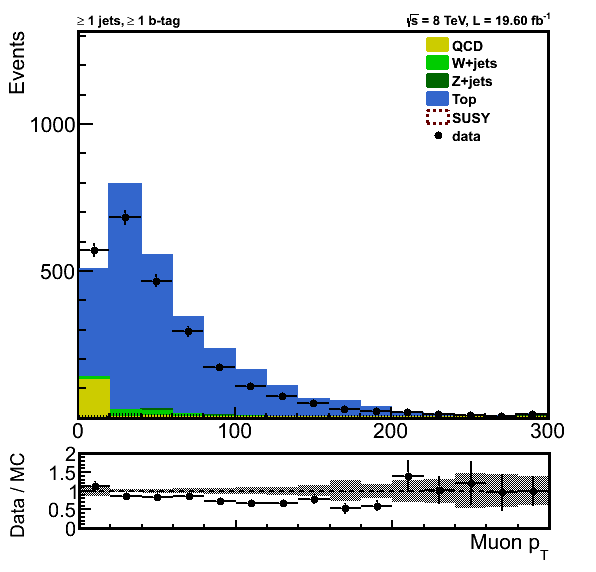
\includegraphics[angle=0,scale=0.35]{llplots_20Invfb/mu_pt.png} \\
\caption{Left: The $p_T$ distribution of the electrons in the events with one electron 
passing all selection cuts but the \mindphifour cut. The reason for this is stated in the text. No $M_{T2}$ cut is applied in 
order to have more statistics. Right: The same plot for muons.}
\label{fig:pt}
\end{figure}

In order to increase the data statistics, the cut on the 
\mindphifour is relaxed. This cut was introduced in the main analysis to suppress the $QCD$ background events. Now that 
the lepton veto is reversed and exactly one lepton is required, the $QCD$ events are still under control. 
Hence relaxing the \mindphifour cut would not be harmful. The only thing which should be taken into account 
is the efficiency of this cut, called as $f$, which is explained in the following.\\
The contribution of the lost lepton background events passing the lepton veto, shown as $N_l^{pass}$, is estimated with the following formula
\begin{eqnarray} 
N_l^{pass}&=&(N_l^{reco}-N_l^{bg})\frac{1}{\varepsilon_l}-(N_l^{reco}-N_l^{bg})\\\nonumber
&=&(N_l^{reco}-N_l^{bg})\frac{1-\varepsilon_l}{\varepsilon_l},\nonumber
\end{eqnarray}
where $N_l^{reco}$ refers to the number of data events with all selection cuts except the 
lepton veto, which is replaced by asking for one lepton. For this set of cuts, the number of background events from processes 
other than $W\rightarrow l\nu_l$ is represented by $N_l^{bg}$ and is taken from MC. The $\varepsilon_l$ contains 
the efficiency for a generated $W\rightarrow l\nu_l$ passing all selection cuts but the inverted lepton veto to have a 
lepton reconstructed. Here, the electron and muon efficiencies are obtained from both $t\bar t$ and $W+jets$ events and a relative contribution is used in the above formula. It should also be noted that, at the generator level, those $t\bar t$ events containing a tau lepton decaying hadronically are vetoed since these kind of events are considered when backgrounds from tau are estimated.\\ 
In order to reduce the signal contamination in the leptonic signal region, a cut on the transverse mass of the 
lepton, $m_T$, is applied which is defined as
$$m_T=\sqrt{2p_T(e,\mu)E_T^{miss}(1-\cos(\Delta\Phi))} < 100\; \rm GeV,$$
where $\Delta\Phi$ is the angle between lepton-$p_T$ and $E_T^{miss}$ in the transverse plane. 
In the $W\rightarrow l\nu_l$ events, the $m_T$ cut represents the transverse mass of 
the $W$ bosons whose distribution drops at $80$ GeV. Hence the leptonic signal events are not 
affected by this cut, while the contamination from SUSY events are strongly suppressed. The 
distribution of the $m_T$ of either electrons or muons in the events with exactly one electron and one muon respectively, are shown in
Figure~\ref{fig:mt}. In this analysis, 
it is found that, e.g. for electron $m_T$ distribution, the $S/B$ decreases from $1.03\%$ to $0.60\%$ when $m_T<100$ GeV cut is introduced. In 
the rest of this section, in addition to all selection cuts, events are required to pass $m_T<100$ GeV cut.\\ 
\begin{figure}[htbp] 
\centering
%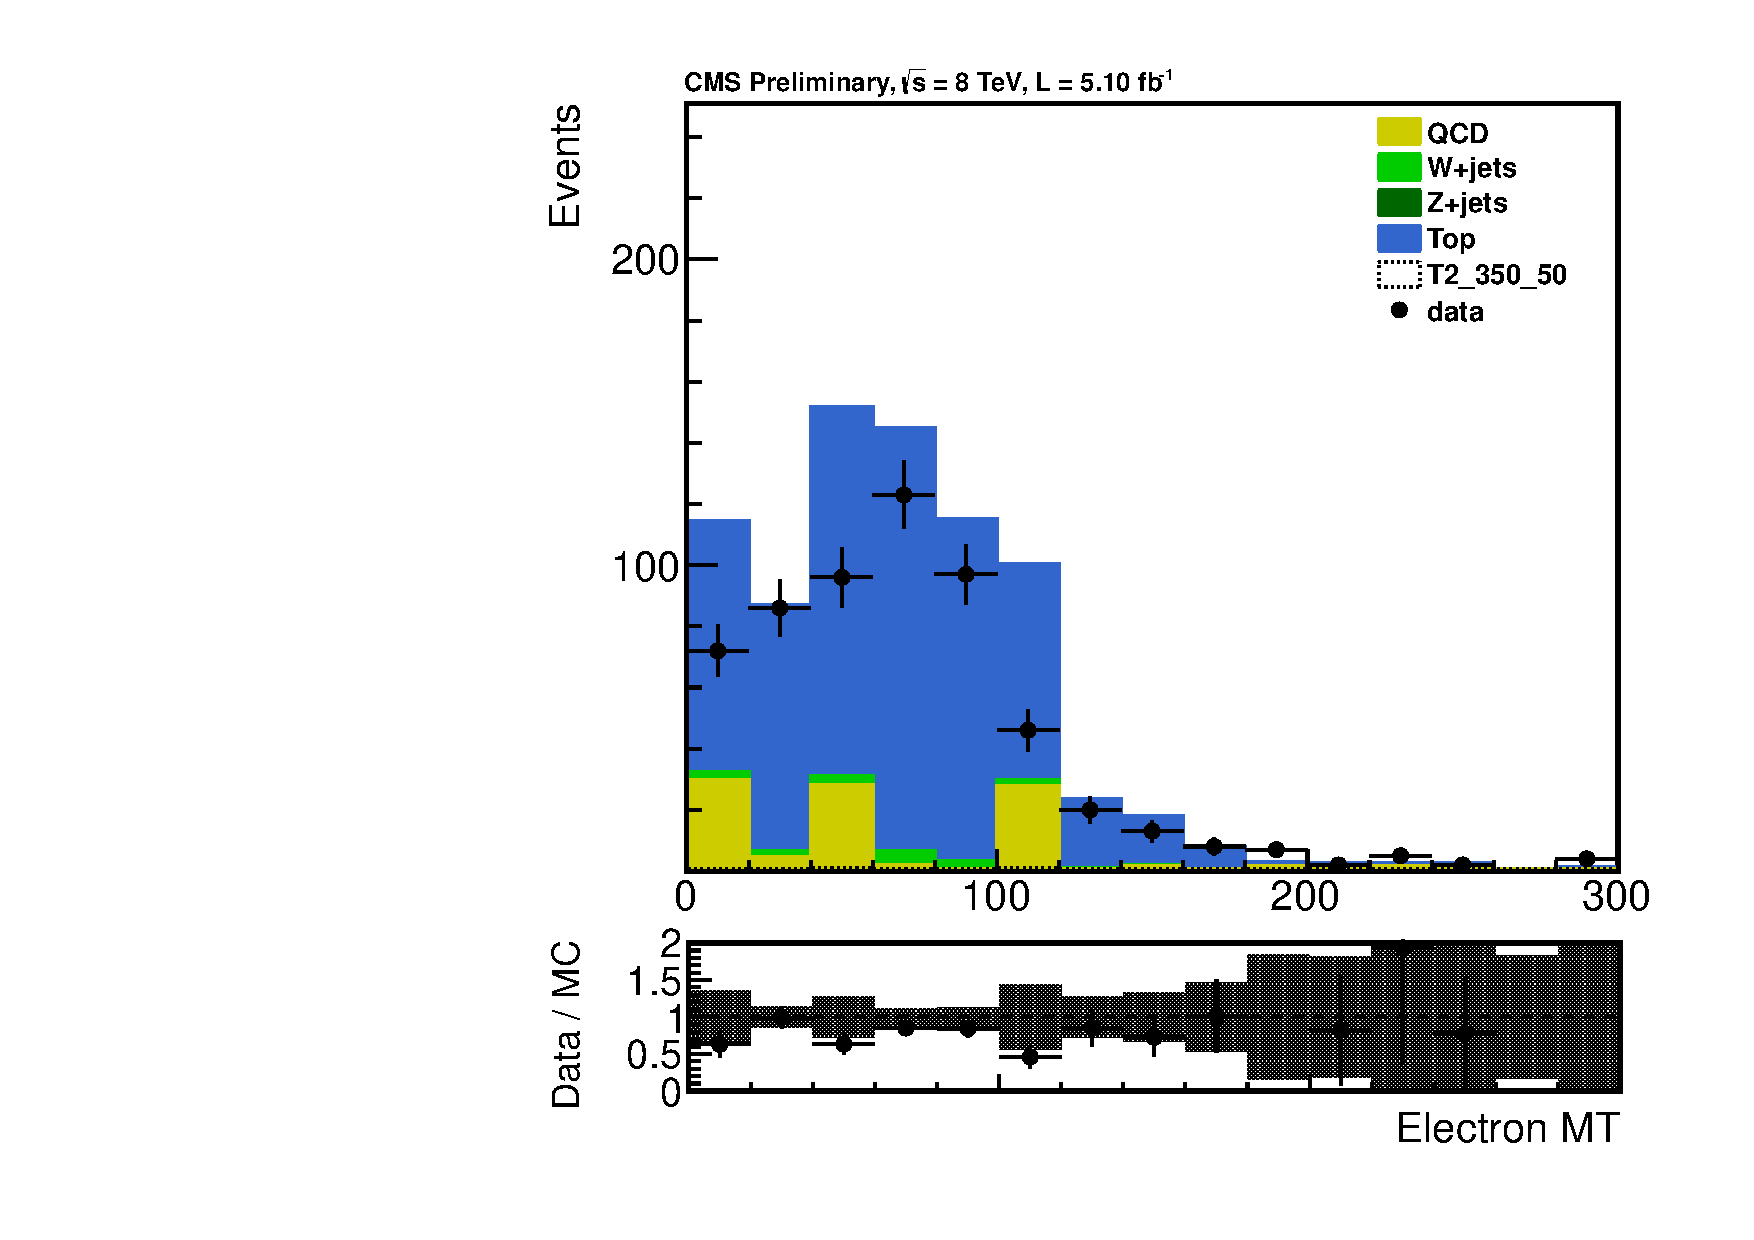
\includegraphics[angle=0,scale=0.39]{myplots/ele_mt.pdf} 
%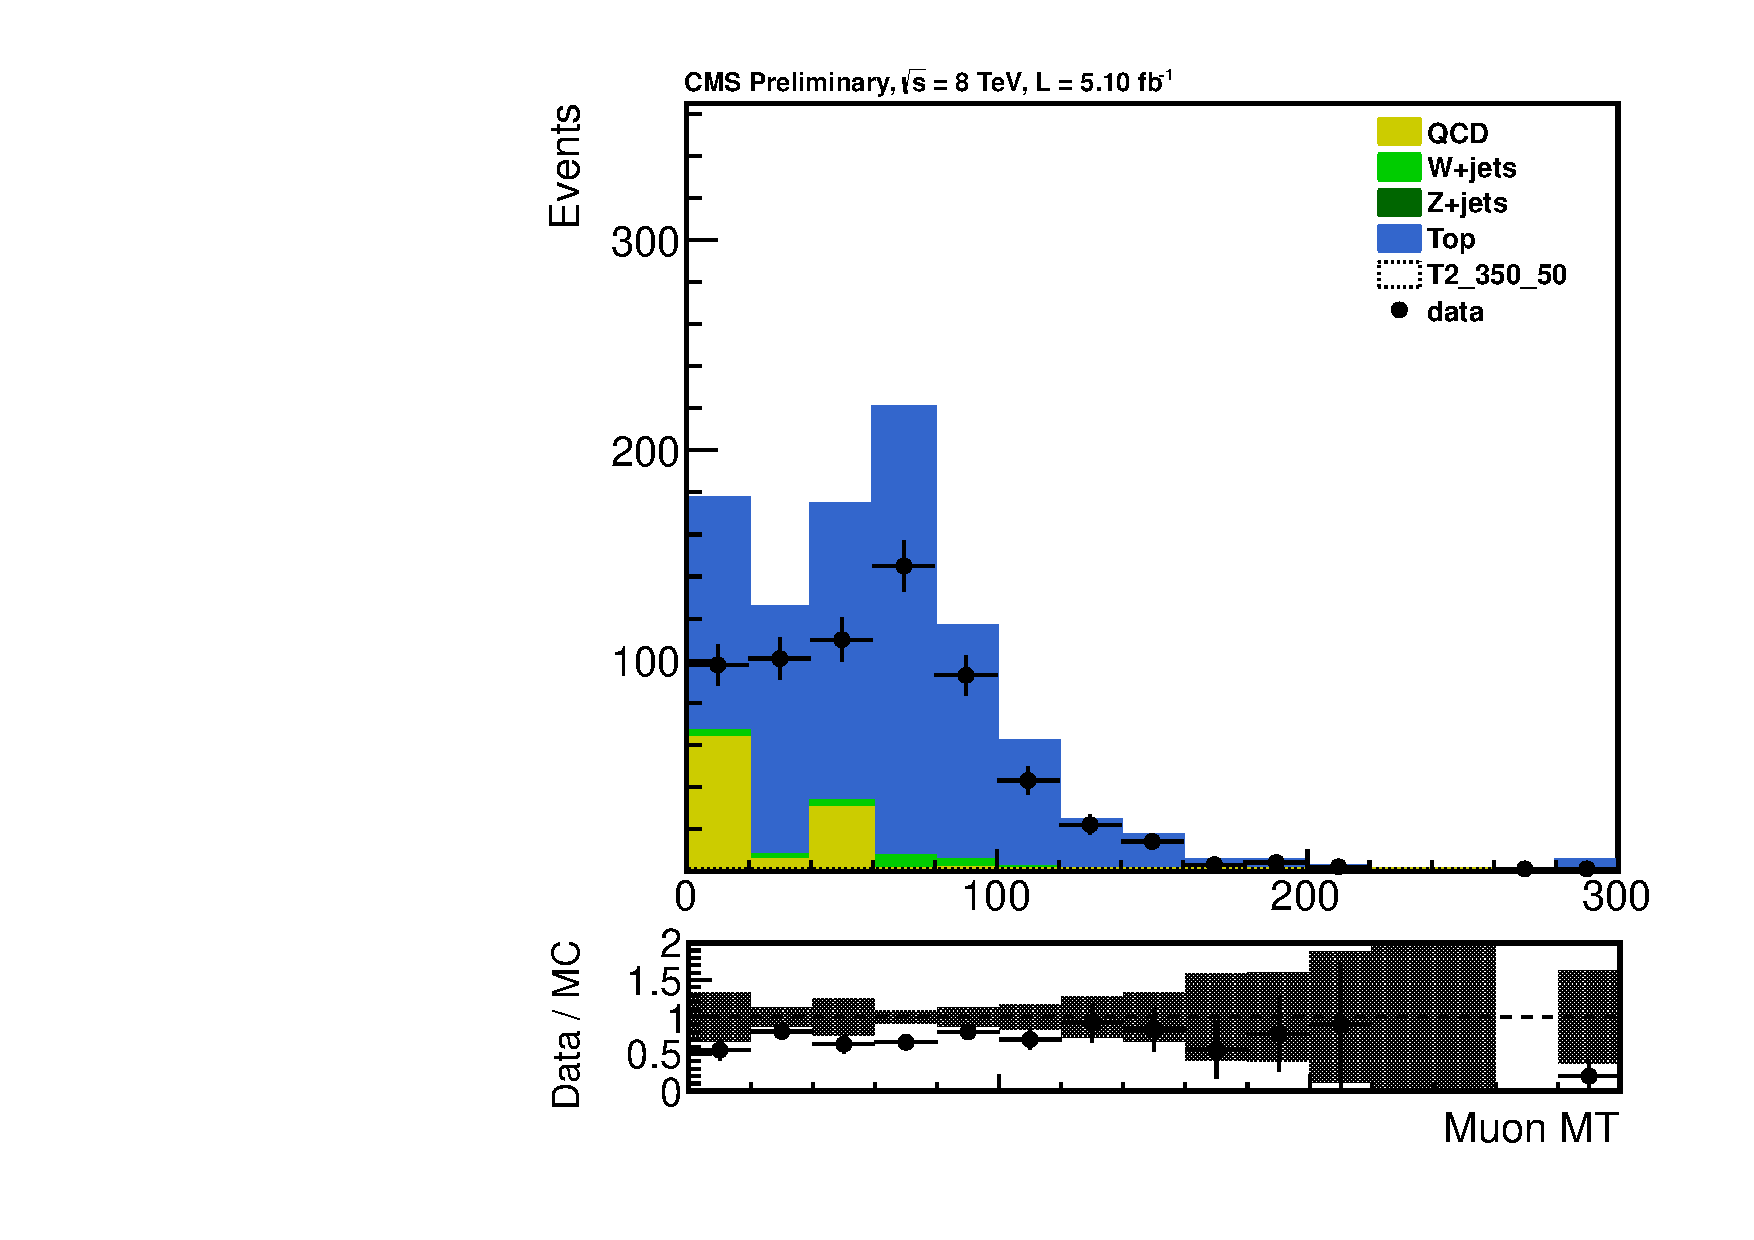
\includegraphics[angle=0,scale=0.39]{myplots/muo_mt.pdf} \\
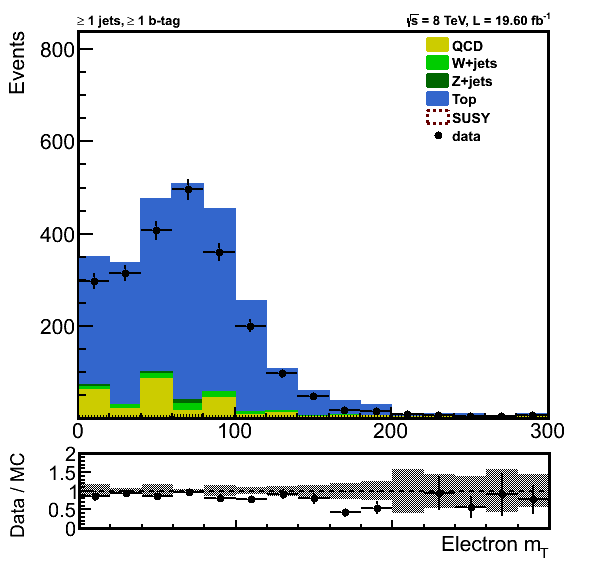
\includegraphics[angle=0,scale=0.35]{llplots_20Invfb/ele_mt.png} 
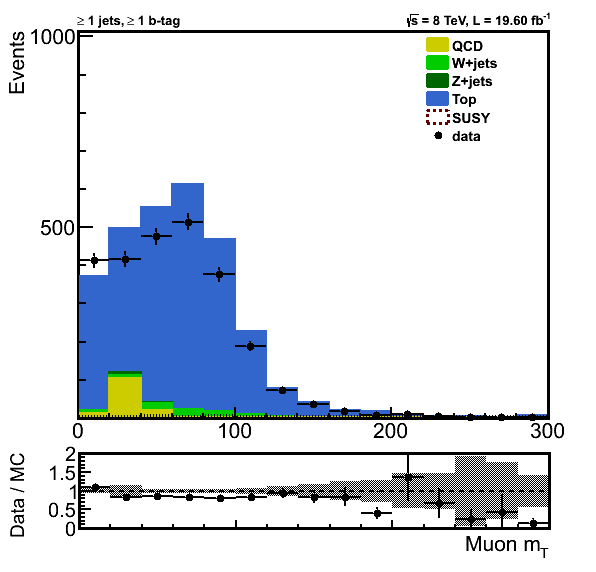
\includegraphics[angle=0,scale=0.35]{llplots_20Invfb/mu_mt.png} \\
\caption{Left: The $m_T$ distribution of the electrons for the events with one electron 
passing all selection cuts but the \mindphifour cut. The reason for this is stated in the text. No $M_{T2}$ cut is applied in 
order to have more statistics. Right: The same plot for muons.}
\label{fig:mt}
\end{figure}

The fraction of events with all selection cuts with respect to the events with all 
selection cuts but the \mindphifour are shown 
in Figure~\ref{fig:fraction} for data and MC. Since in the signal region, defined as region with $M_{T2}>125$ GeV, the ratios become flat; one can fit the ratios with a straight line. For both electrons and muons, the MC ratio is fitted and the fitted parameters $f$ are quoted in Table~\ref{tbl:fitvalues}.\\
\begin{figure}[htbp] 
\centering
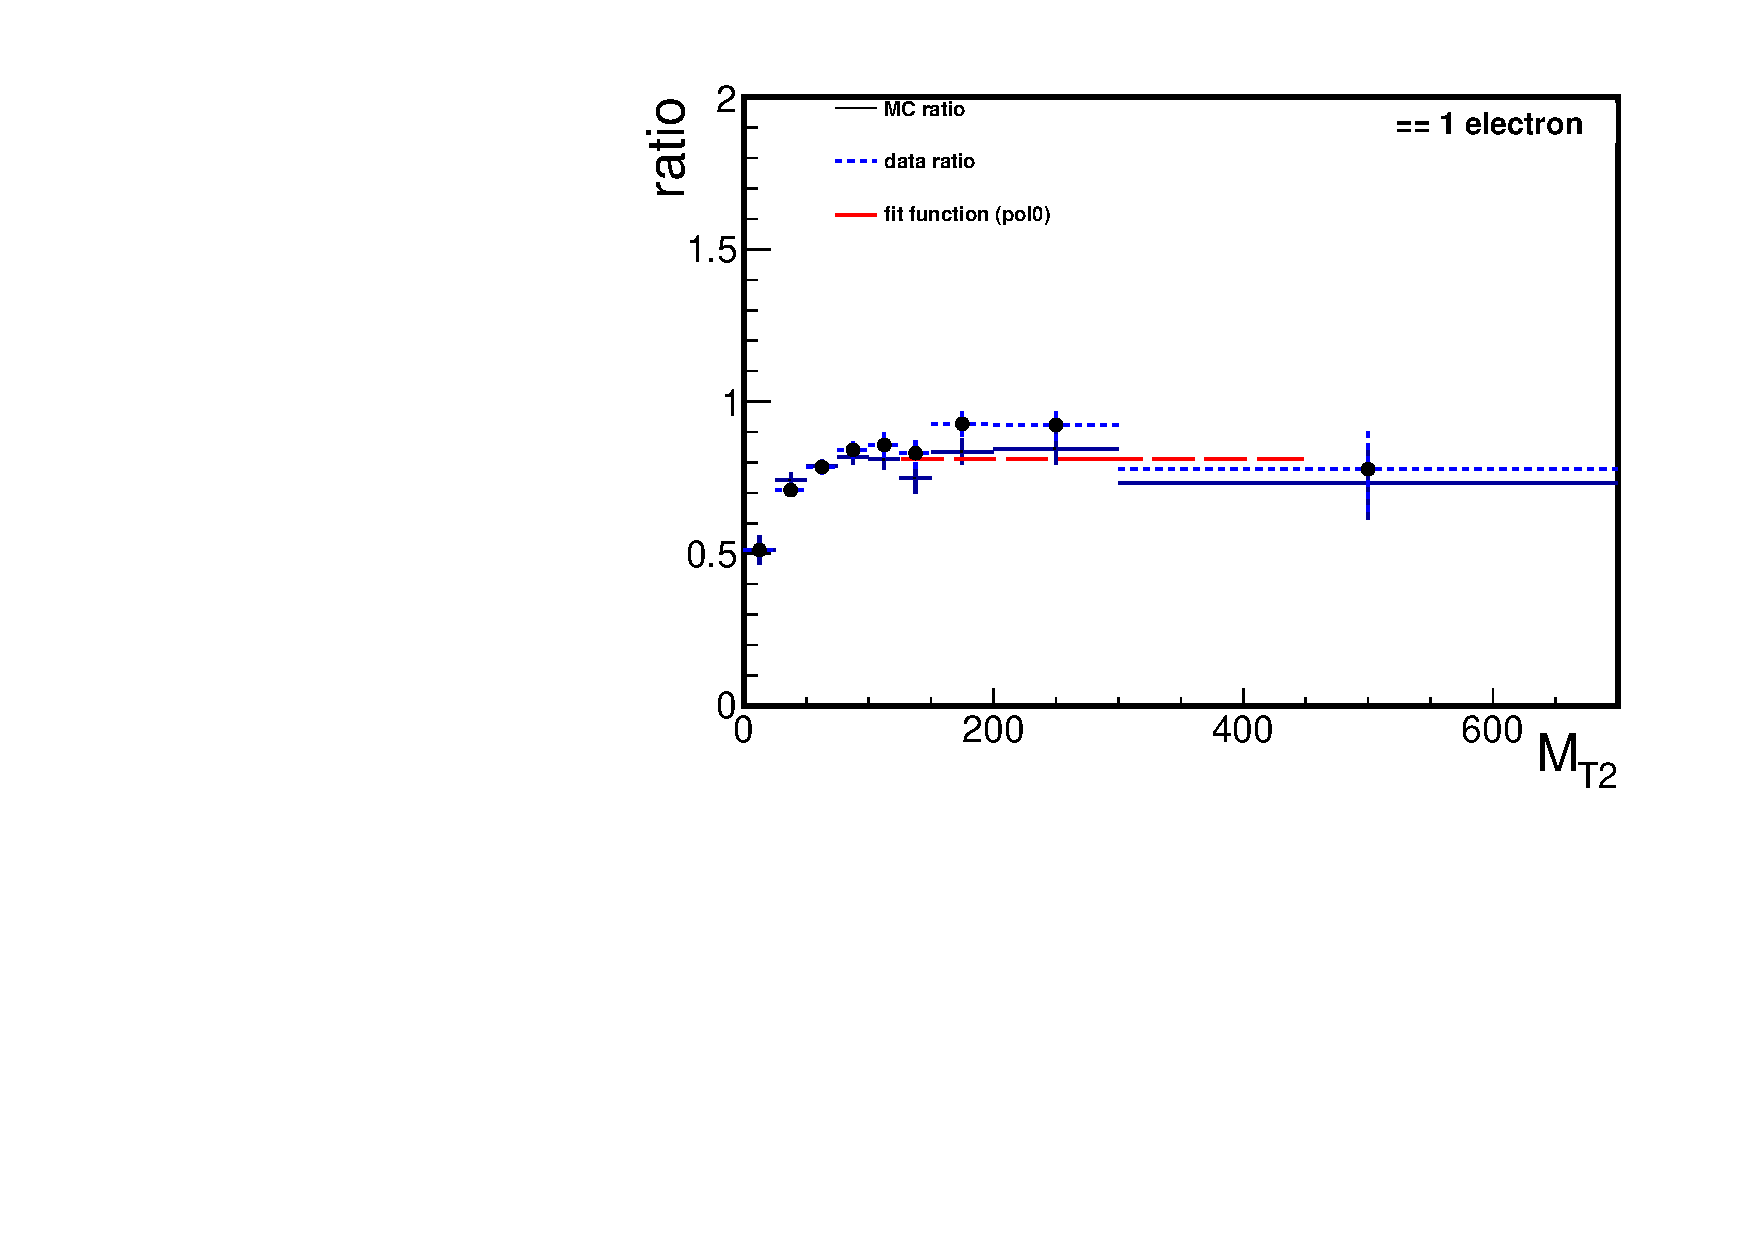
\includegraphics[angle=0,scale=0.39]{llplots_20Invfb/ele_ratio.pdf} 
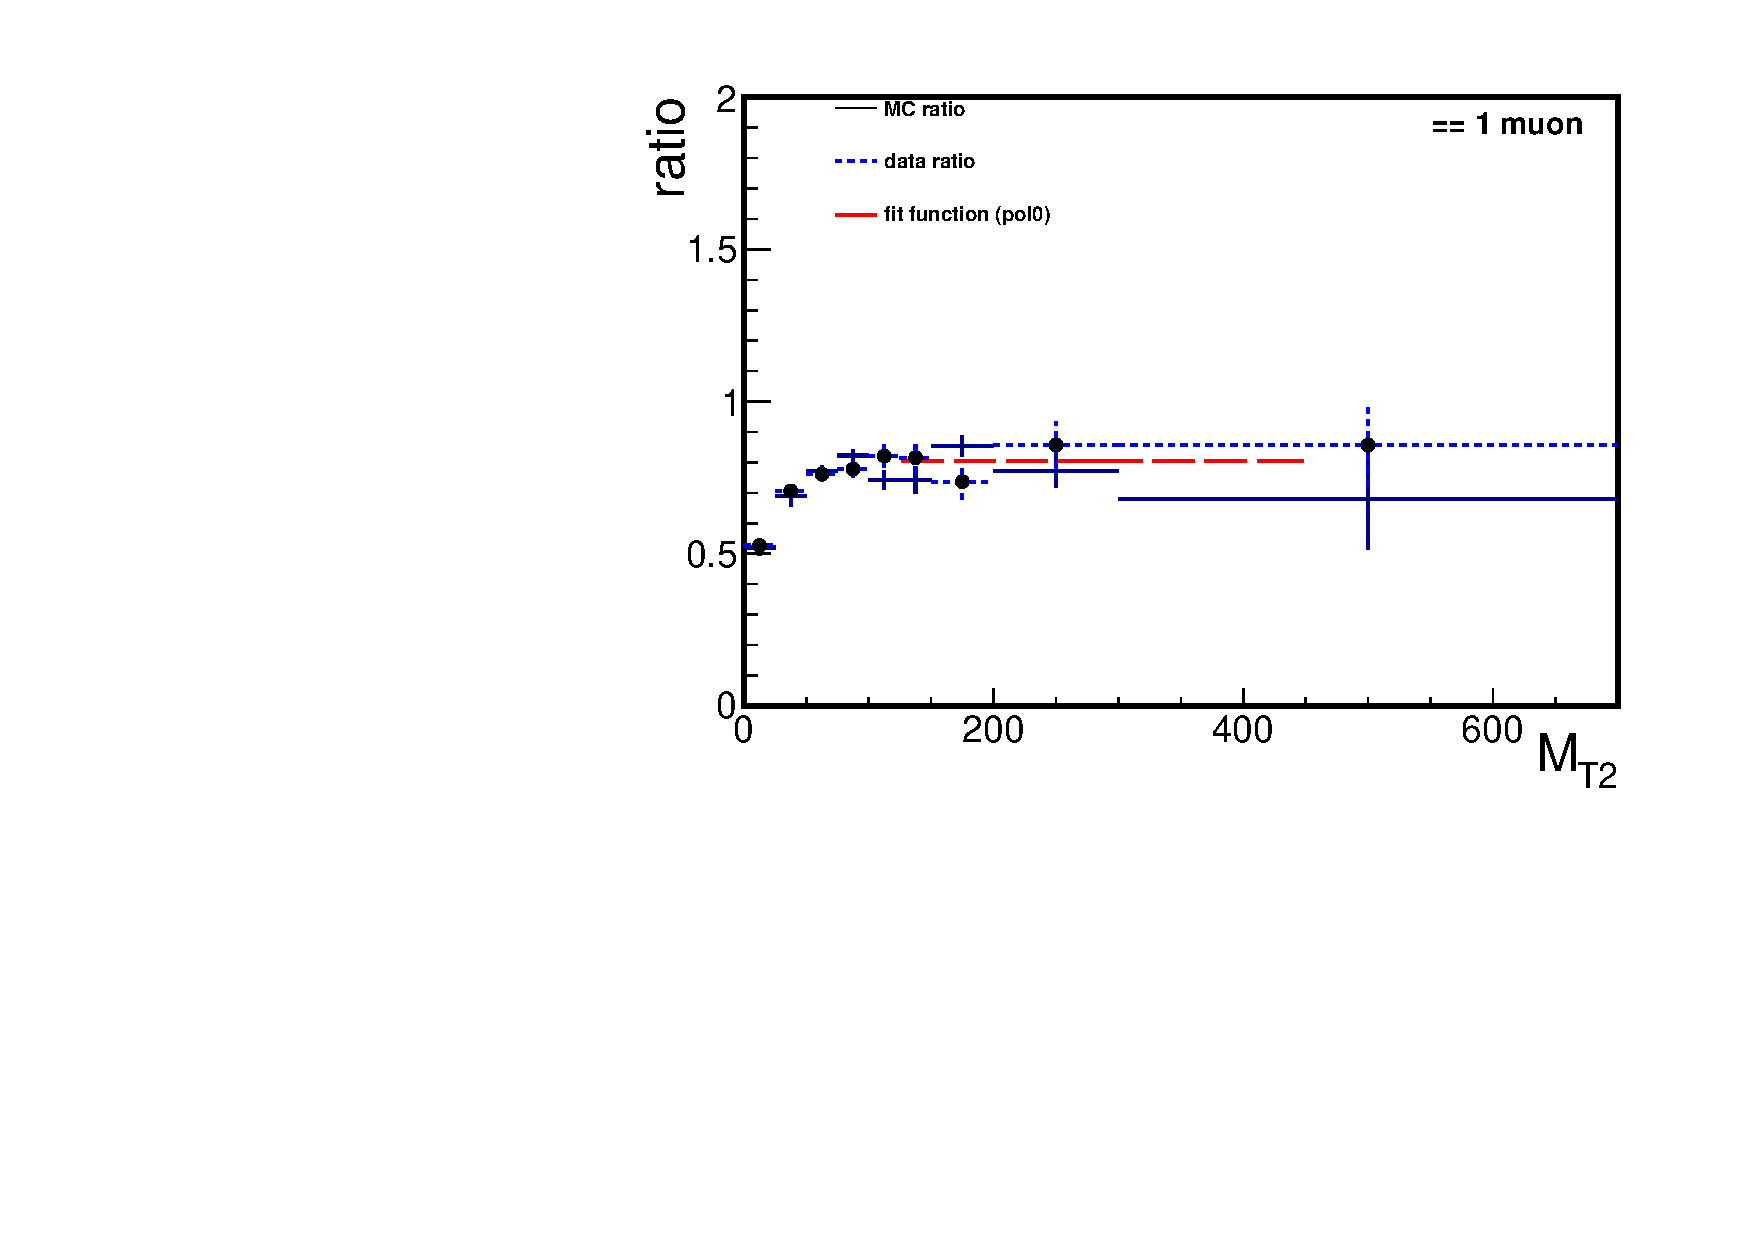
\includegraphics[angle=0,scale=0.39]{llplots_20Invfb/mu_ratio.pdf} \\
\caption{Left: Ratio between events with one electron passing all selection cuts 
versus events with one electron passing all selection cuts but the 
\mindphifour for data (blue) and MC (black). 
The fit line for the MC ratio over all $M_{T2}$ signal bins is drawn in red. Right: The same plot for events with one muon.}
\label{fig:fraction}
\end{figure}

\begin{table}[hbtp]
\begin{center}
\small
\begin{tabular}{lcc}\hline\hline
   &  electrons    &   muons   \\ \hline
Fit value for the ratio $f$    & $0.811 \pm 0.028$     &   $0.804 \pm 0.024$    \\ \hline\hline
\end{tabular}
\caption{Fit values $f$ obtained from the MC ratios for electrons and muons.}
\label{tbl:fitvalues}
\end{center}
\end{table}

The results of estimation of the lost lepton background events from data are summarized in 
Table~\ref{tbl:llestimation}. It should be mentioned that, the number of data events with 
one lepton selection and its corresponding background events are obtained from the relaxed 
cut selection, where \mindphifour is dropped. Therefore the prediction 
is corrected back by multiplying the event yield with the fitted ratio value $f$.\\ 
\begin{table}[hbtp]
\begin{center} 
\begin{tabular}{lccccc} 
\hline\hline 
& %$N^{W,Top}$ MC &
 $N^{reco}$ & $N^{bg}$ & $R_{LL}$ & $N^{pass}$ MC-Truth & $N^{pass}$ data-prediction \\\hline 
electrons &%&
&&&&\\\hline 
& %$38.94$ &
 $129$ & $20.78$ & $1.30\pm0.17$ & $189.32\pm10.86$ & $139.63\pm 14.72(stat)\pm 33.48 (sys)$\\\hline\hline 
muons &%&
&&&&\\\hline 
& %$45.55$ &
 $150$ & $25.42$ & $0.73\pm0.13$ & $133.08\pm 9.16$ & $91.29\pm 8.97 (stat)\pm 24.97 (sys)$\\ 
\hline\hline 
\end{tabular} 
\caption{Data-Driven Estimation of Lost Lepton from $W+$jets and $t(\bar t)$ for electrons and muons. The lost lepton ratio $R_{LL}$ is given by $f\frac{1-\varepsilon_l}{\varepsilon_l}$.}
\label{tbl:llestimation}
\end{center} 
\end{table} 

It should be noted that for the systematic uncertainty, two possible sources are taken into account. The first one is a systematic uncertainty of 100\% on the number of backgrounds. The second one is a systematic uncertainty of 5\%, considered when calculating the efficiencies $\varepsilon_l$ from MC, to account for possible difference between data and simulation. Considering the uncertainties, the data-driven estimation for the lost lepton channel is slightly less than MC truth. We use MC estimation in limit calculation to be on the safe side.


\subsection{Estimation of the Tau Leptons}
\label{sect:tau}
Tau leptons can decay hadronically and appear as a thin jet and enter the hadronic searches. 
To estimate the contamination from such events a method similar to what is used for the lost lepton background is used here. The number of 
events with exactly one real tau is corrected by accounting for the reconstruction and acceptance efficiencies. In the other words:
\begin{linenomath}
\begin{equation}
	N_{W\rightarrow{\tau\nu}} = \frac{N_{\tau}^{reco} - N_{\tau}^{bg}}{\varepsilon_{\tau}},
	\label{eq:TauEstimation}
\end{equation}
\end{linenomath}
where $N_{\tau}^{reco}$ is the number of events with one reconstructed tau, $N_{\tau}^{bg}$ is the number of events with a 
fake tau and $\varepsilon_{\tau}$ denotes the probability for a generated
$W \rightarrow \tau\nu, \ \tau \to had$ event passing the selection cuts to have a reconstructed and identified tau. 
The efficiency $\varepsilon_{\tau}$ is extracted from simulation. In average, $\varepsilon_{\tau}$ is found to be $\sim24$\%. 5\% systematic 
uncertainty is assigned to this value to take into account the differences between data and MC.
The transverse mass (\mt) of the system of the reconstructed tau and MET is forced to be less than 100 GeV/$c^2$ to decrease 
the signal contamination.  The number of events with a fake tau, $N_{\tau}^{bg}$ is found from the MC simulation and a 50\% systematic 
uncertainty is assigned to this value.

The \mttwo distribution of the events with all selection cuts which have an
identified tau in the final state is shown in Figure \ref{fig:MT2Tau}.
\begin{figure}[!htb]
\centering
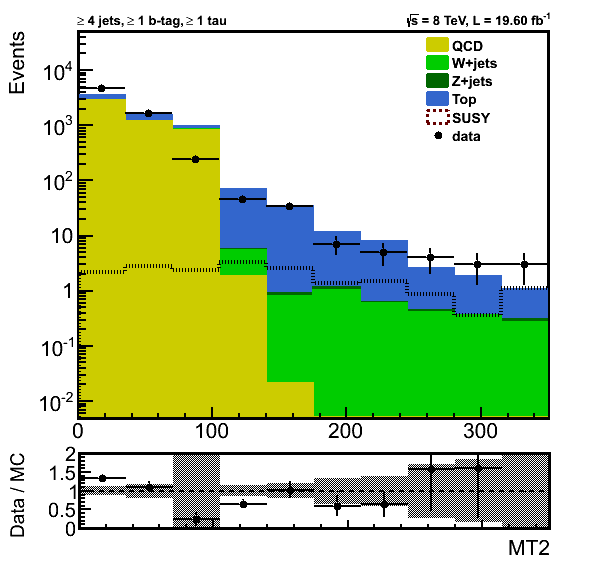
\includegraphics[width=0.49\textwidth]{figs/MT2Tau.png}
\caption{\mttwo distribution for events with at least one tau in data and MC with all selection cuts.}
\label{fig:MT2Tau}
\end{figure}
Scale factors of the tau selection are not applied and it can be the source of the discrepancies between data and MC. 
In Table~\ref{table:Tau_yield} 
\begin{table}[!htb]
\begin{center}
\small
\begin{tabular}{lcccccc}
\hline\hline
\mttwo (GeV)   &  QCD   & Z+Jets & W+Jets & Top & MC(sum) & data \\
\hline
 full range & 1480.06 & 0.35 & 9.59 & 417.80 & 1907.79 $\pm$ 182.88 & 2309.00\\
$125-\infty$ &   1.46 & 0.08 & 0.94 &  20.13 &   22.61 $\pm$ 4.57   & 21.00\\
\hline\hline
\multicolumn{7}{c}{cut on \mindphifour is relaxed}\\
\hline\hline
$125-\infty$ &      6.21 & 0.11 & 2.03 & 31.91 & 40.25 $\pm$ 6.18 & 34.00\\
\hline\hline
\end{tabular}
\caption{MC and data event yields in full range and signal region. The last row shows the yields after relaxing the cut.
The error on the total background is purely statistical.}
\label{table:Tau_yield}
\end{center}
\end{table}
contribution of different samples in the plot of Figure \ref{fig:MT2Tau} is shown. It can be seen that the statistics in the signal
region is poor. To decrease the uncertainties of the predictions, the cut on  \mindphifour is relaxed. 
The last row of the table shows the statistics after this relaxation. The scale factor to compensate this relaxation is 
read from MC.

Table \ref{table:MT2TauCutsRelaxed} 
\begin{table}[!htb]
\begin{center}
\small
\begin{tabular}{lccc}
\hline\hline
  \mttwo bin  &      MC Truth     &         Prediction in MC       & Prediction in Data \\\hline
$125-\infty$   &  78.40 $\pm$ 9.64 &  77.38 $\pm$ 19.94 $\pm$ 35.63 & 57.20 $\pm$ 18.83 $\pm$ 33.00\\
\hline\hline
\end{tabular}
\caption{Prediction of the tau contamination in the signal region in both data and MC.}
\label{table:MT2TauCutsRelaxed}
\end{center}
\end{table}
shows the performance of the method on MC and data. The quoted uncertainties of the predictions are statistical and systematical, respectively.

\subsection{Estimation of Invisible Z Background from Data Using W +jets Events}
\label{sect:znunu}
To estimate $Z\rightarrow\nu\bar{\nu}$ background we use $W\rightarrow\mu\nu$+jets events. The kinematics of leptons as well as the jets are very similar in both Z+jets and W+jets processes. Besides, the larger cross-section of W+jets allows for a more precise estimation of
$Z\rightarrow\nu\bar{\nu}$.  This is a well studied method in various analyses within the CMS Collaboration (see e.g. \cite{CMS-PAS-SUS-08-002,CMS-PAS-SUS-10-001,CMS-PAS-SUS-11-005}).
To make the event kinematics compatible from the \met point of view, the \pT of muon is added to the one of neutrino in W+jets events. The \mttwo variable and other quantities related to \met are recalculated accordingly.
This estimation can be described as:

\begin{linenomath}
\begin{equation}
\label{eq:ZinvEst}
N_{Z\rightarrow\nu\bar{\nu}}(est) = N_{W (\mu\nu)} R^{MC} \frac{1}{\epsilon_{acc}\epsilon_{reco/iso}}.
\end{equation}
\end{linenomath}
where,\\
$\bullet \hspace{5pt} \epsilon_{acc}$ is the muon acceptance derived from MC.\\
$\bullet \hspace{5pt} \epsilon_{reco/iso}$ is the muon reconstruction and isolation efficiency, taken from data using the Tag\&Probe method.\\
$\bullet \hspace{5pt} R^{MC}$ corrects kinematic, selection and cross-sections differences between $Z\rightarrow\nu\bar{\nu}$ and $W\rightarrow\mu\nu$+jets processes.\\
$\bullet \hspace{5pt} N_{W (\mu\nu)}$ is the number of selected $W\rightarrow\mu\nu$+jets events.\\

The selection is similar to the one of signal where the lepton veto is reduced to an electron veto. In addition we request for the presence of exactly one reconstructed muon passing all the quality and isolation cuts, with $p_T >10$ GeV and $|\eta| <2.4$. The W-boson transverse mass (using default \met) is required to be $\mt < 100$ GeV in order to reduce other backgrounds and signal contaminations. To enrich the sample with W+jets and to reject $t\bar{t}$ events, we veto events with at least one b-tagged jet where the medium working point of CSV b-tagging algorithm is applied on jets with $p_T >20$ and $|\eta| <2.4$. The results of this selection for MC samples and data are summarized in Table~\ref{tab:WenrichYields}. The distributions of muon \pT, \mttwo and \mt for this region are shown in Figures~\ref{fig:WenrichedPlots}a,~\ref{fig:WenrichedPlots}b and~\ref{fig:WenrichedPlots}c and as it is seen there is a good agreement between data and MC in W enriched region.\\
\begin{figure}[!h]
\begin{center}$
\begin{array}{cc} 
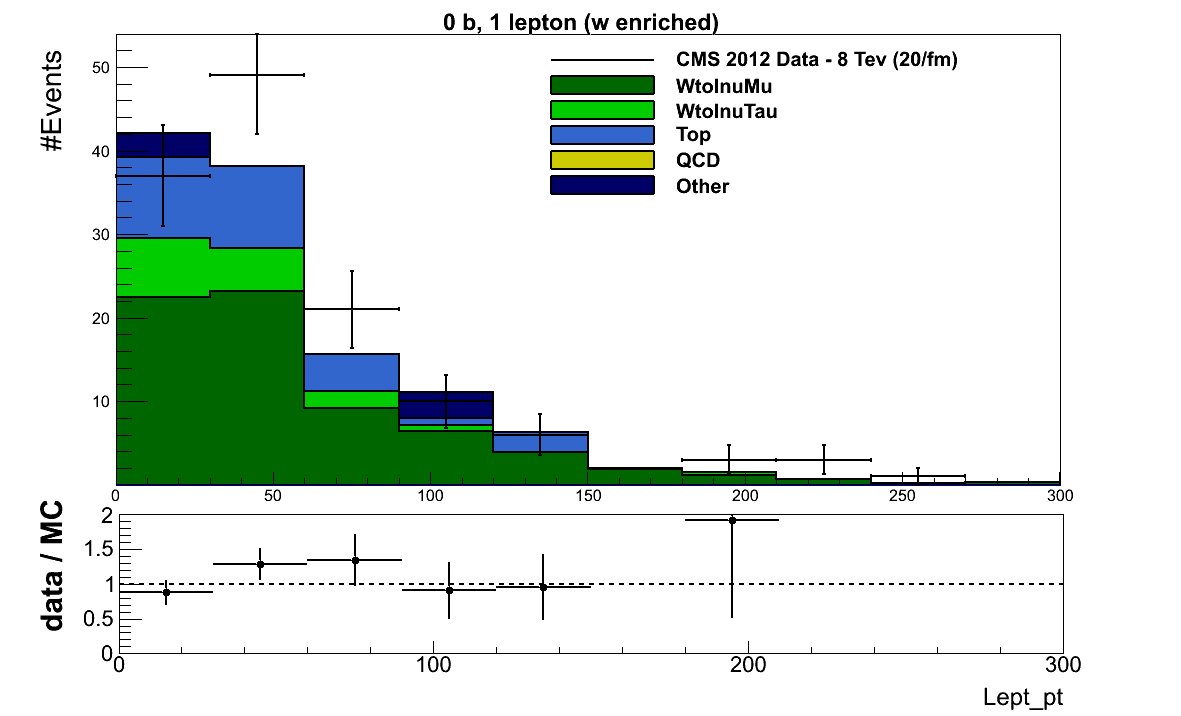
\includegraphics[angle=00,width=0.5\textwidth]{figs/Lept_Pt_0b_Mod.png}&
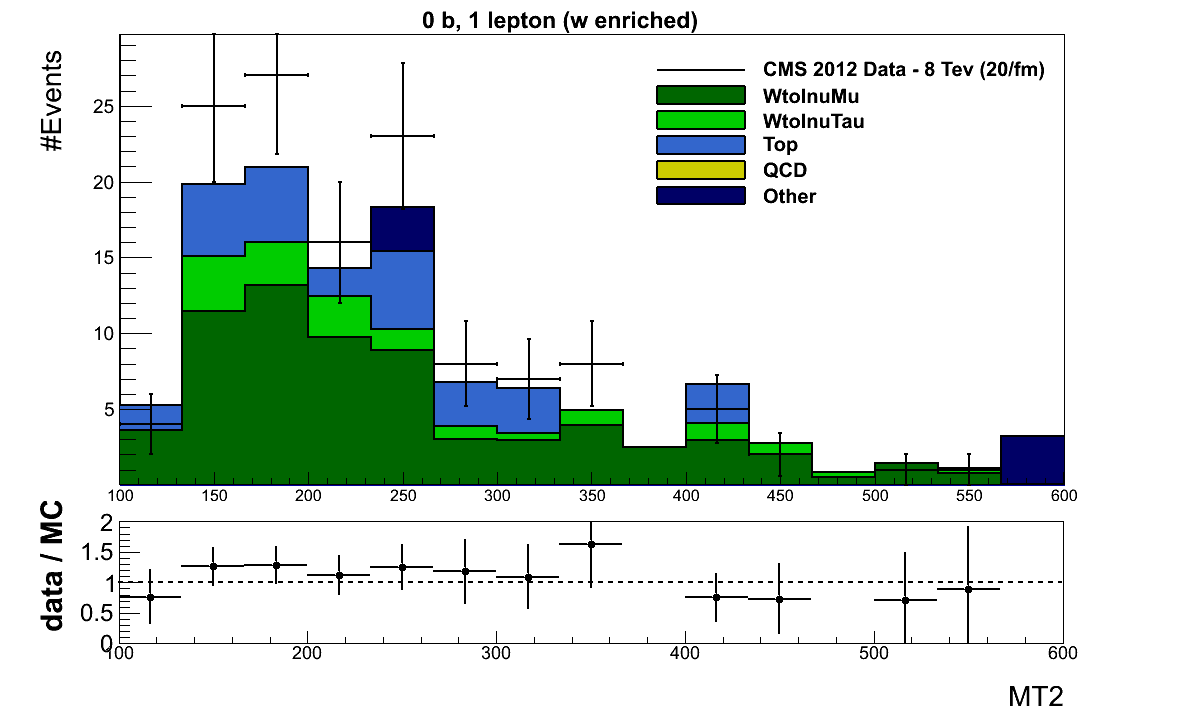
\includegraphics[angle=00,width=0.5\textwidth]{figs/MT2_0b_Mod.png}\\
	\mbox{\small{(a)}} & \mbox{\small{(b)}} \\
\end{array}$
\end{center}
\begin{center}$
\begin{array}{c}
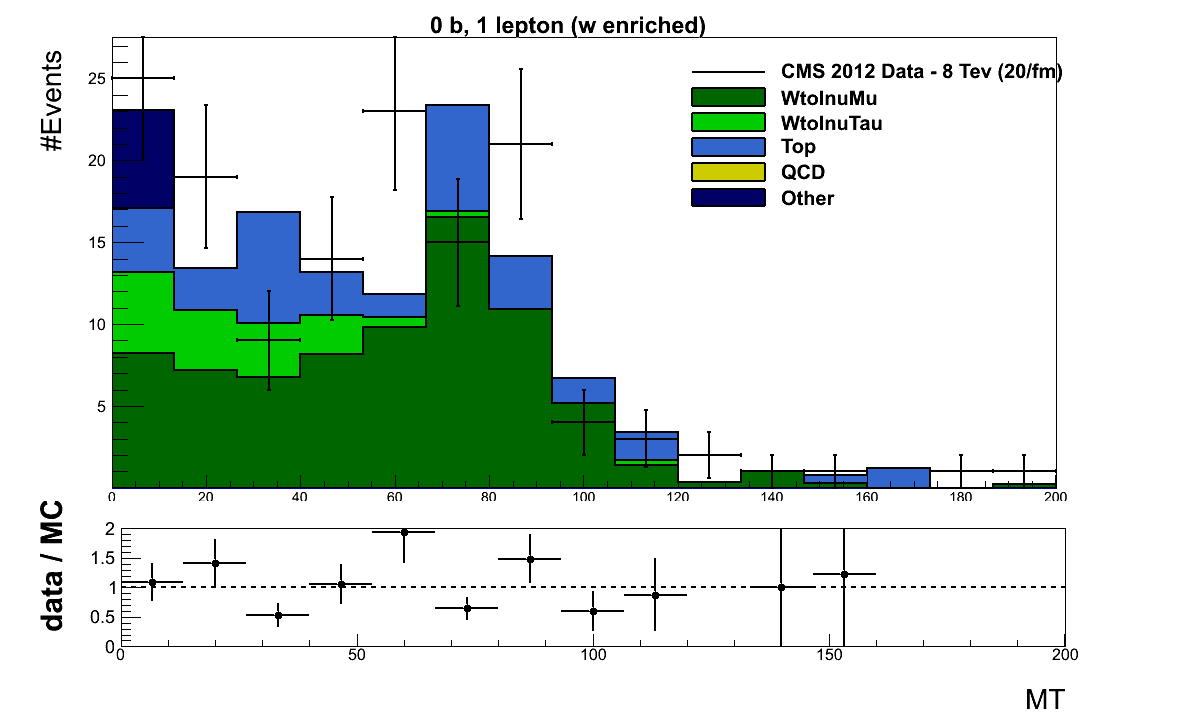
\includegraphics[angle=00,width=0.5\textwidth]{figs/MT_0b_Mod.png}\\
	\mbox{\small{(c)}}  \\
\end{array}$
\end{center}
\caption{Muon \pT, \mttwo and \mt distributions for W-enriched region}
\label{fig:WenrichedPlots}

\end{figure}


%..........................
\begin{table}[!htb]
\setlength{\tabcolsep}{2pt}
\small
\begin{center}

\begin{tabular}{lccccccccc} 
\hline\hline
& WtolnuMu& WtolnuTau& QCD& Zinv& Top& SMS& Other& MC& data \\ \hline \hline
 All events ($\rm jets\geq X$) & 145.81  & 230.75  & 462.23  & 235.41  & 1314.11  & 0.00 & 184.86  & 2573.17 +- 80.53 & 2510.00  \\
 %$Minimum DPhi(\met,jet) > 0.3$ & 40.56  & 65.36  & 146.80  & 65.29  & 328.56  & 0.06  & 50.78  & 697.35 $\pm$ 52.10 & 597.00  \\ 
 %HBHE noise veto & 40.56  & 65.36  & 146.80  & 65.29  & 328.56  & 0.06  & 50.78  & 697.35 $\pm$ 52.10 & 597.00  \\ 
 %$\met > 30GeV$ & 40.56  & 65.36  & 146.80  & 65.29  & 328.56  & 0.06  & 50.78  & 697.35 $\pm$ 52.10 & 597.00  \\ 
% $VectorSumPt < 70$ & 40.56  & 65.36  & 146.80  & 65.29  & 328.56  & 0.06  & 50.78  & 697.35 $\pm$ 52.10 & 597.00  \\ 
Analysis selection cuts& 145.81  & 230.75  & 462.23  & 235.41  & 1314.11  & 0.00 & 184.86  & 2573.17 +- 80.53 & 2510.00  \\ 
Lepton Veto & 145.81  & 214.43  & 459.75  & 235.29  & 1068.30  & 0.00 & 96.65  & 2220.23 +- 78.92 & 2192.00  \\ 
Lepton Selection & 91.76  & 17.61  & 0.74  & 0.11  & 277.43  & 0.00 & 6.00  & 393.65 +- 16.96 & 329.00  \\ 
$m_T < 100\, \rm GeV$ & 83.26  & 17.30  & 0.74  & 0.06  & 241.95  & 0.00 & 6.00  & 349.30 +- 15.99 & 293.00  \\  
$b$-jets Selection & 69.67  & 15.29  & 0.00  & 0.03  & 27.85  & 0.00 & 6.00  & 118.83 +- 8.25 & 130.00  \\ 
 \mttwo  100 - 150 GeV & 8.97  & 1.56  & 0.00  & 0.00  & 4.67  & 0.00  & 0.00  & 15.20 +- 2.69 & 12.00  \\ 
 \mttwo  150 - 200 GeV & 19.28  & 4.94  & 0.00  & 0.03  & 6.61  & 0.00 & 0.00  & 30.86 +- 3.67 & 44.00  \\
 \mttwo  200 - 275 GeV & 19.45  & 4.09  & 0.00  & 0.00  & 8.71  & 0.00 & 2.88  & 35.14 +- 4.75 & 41.00  \\ 
 \mttwo  275 - 375 GeV  & 9.80  & 2.25  & 0.00  & 0.00  & 4.19  & 0.00 & 0.00  & 16.24 +- 2.71 & 21.00  \\ 
 \mttwo  375 - 500 GeV & 7.39  & 2.08  & 0.00  & 0.00  & 2.57  & 0.00 & 0.00  & 12.04 +- 2.33 & 7.00  \\ 
 $\mttwo > 500$ GeV & 4.08  & 0.37  & 0.00  & 0.00  & 1.10  & 0.00  & 3.12  & 8.67 +- 3.43 & 5.00  \\
\hline\hline 
\end{tabular} 
\caption{Yields for the W-enriched selection}
\label{tab:WenrichYields}
\end{center} 
\end{table}

\subsubsection{\texorpdfstring{$\rm{t\bar{t}}$ background estimation in W-enriched sample}{tt background estimation in W-enriched sample}}

Despite of b-tag veto some top events remain in W enriched region. The contribution of $t\bar{t}$ is estimated from data while for the rest of backgrounds we trust on simulation. The b-tag veto is relaxed and at least one b-jet is requested to obtain a sample enriched in top events. The selection results are shown in Table~\ref{tab:toEnrichyields}. To find out the number top events in b-tag veto region (W enriched), b-tagging (in)efficiency has to be considered. This process can be described as:
%.................
\begin{linenomath}
\begin{equation}
\label{eq:topEst}
N_{top}(b-veto) = N_{top}(\geq1b-tag) \frac{\epsilon(b-veto)}{\epsilon(\geq1b-tag)},
\end{equation}
\end{linenomath}
where the $\epsilon(b-veto)$ and $\epsilon(\geq1b-tag)$ are the efficiencies of vetoing or selecting b-tagged events and are taken from simulation, thus corrected by the data-simulation scale factors given by the b-tag POG for the CSVE (0.963 $\pm$ 0.020) and CSVT(0.947 $\pm$ 0.025) working points, respectively~\cite{CMS-BTV-AN-12-470}. As it is apparent from Table~\ref{tab:toEnrichyields} there is a good agreement between data and MC in top-enriched region and also the Muon \pT, \mttwo and \mt distributions are shown in Figures~\ref{fig:topEnrichedPlots}a,~\ref{fig:topEnrichedPlots}b and~\ref{fig:topEnrichedPlots}c, respectively.


\begin{figure}[!h]
\begin{center}$
\begin{array}{cc} 
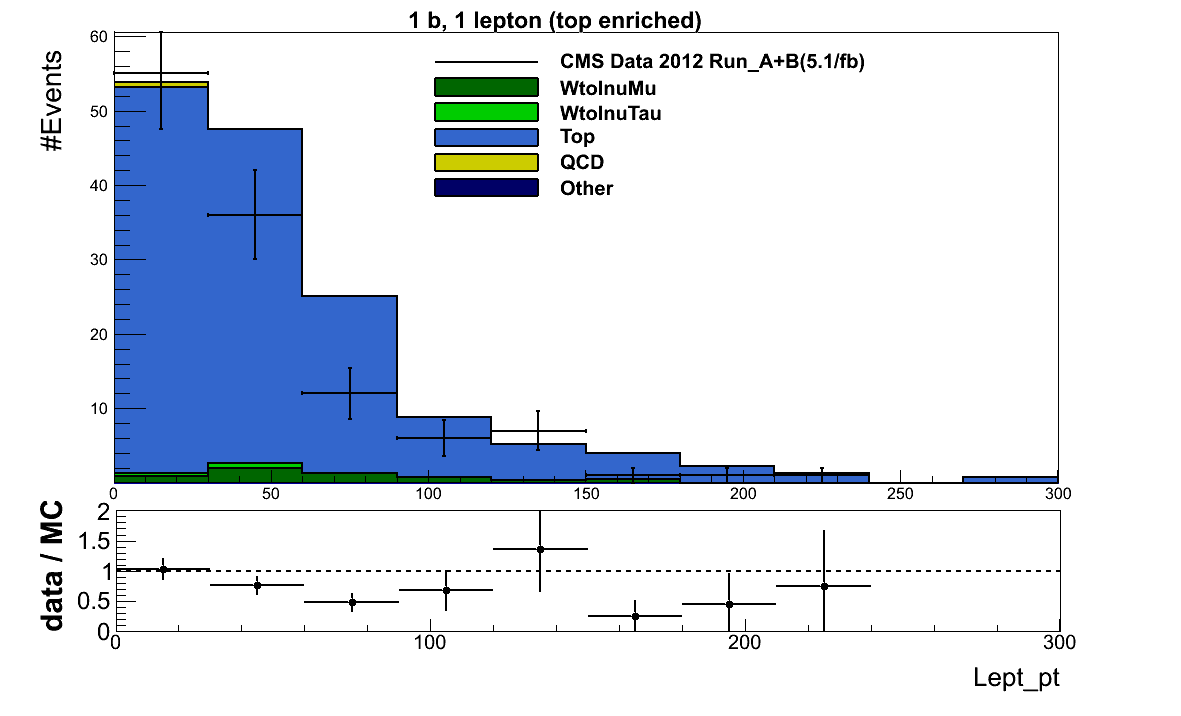
\includegraphics[angle=00,width=0.5\textwidth]{figs/Lept_Pt_1b_Mod.png}&
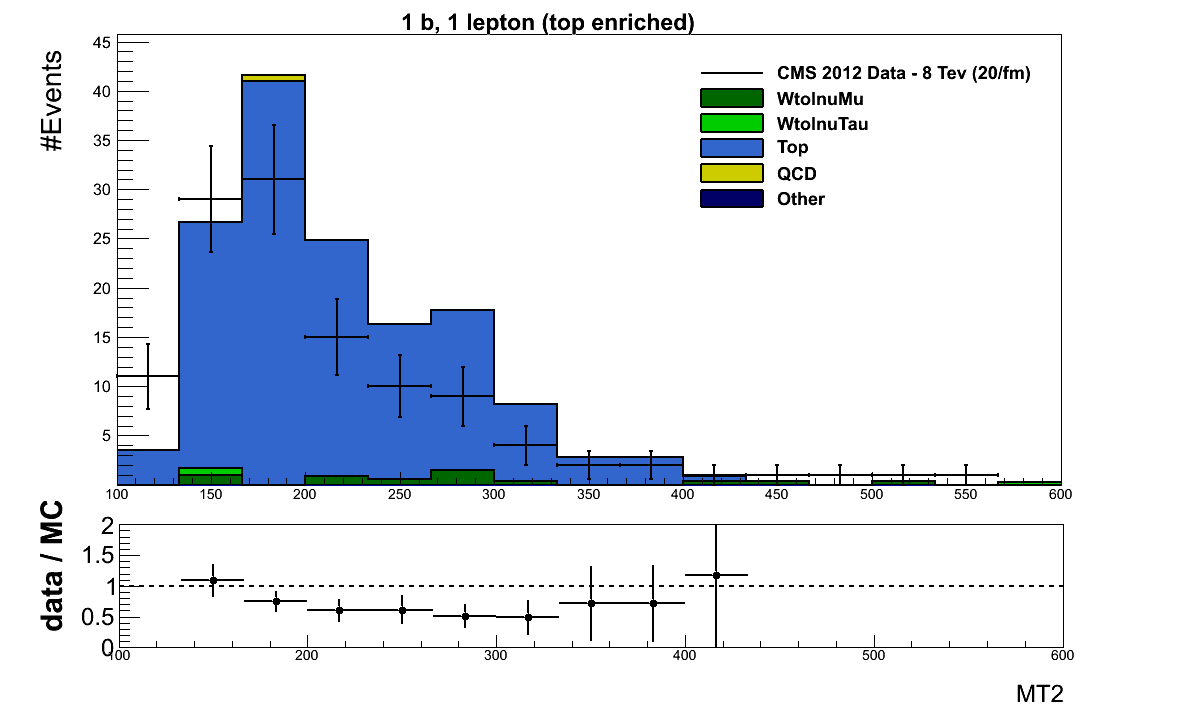
\includegraphics[angle=00,width=0.5\textwidth]{figs/MT2_1b_Mod.png}\\
	\mbox{\small{(a)}} & \mbox{\small{(b)}} \\
\end{array}$
\end{center}
\begin{center}$
\begin{array}{c}
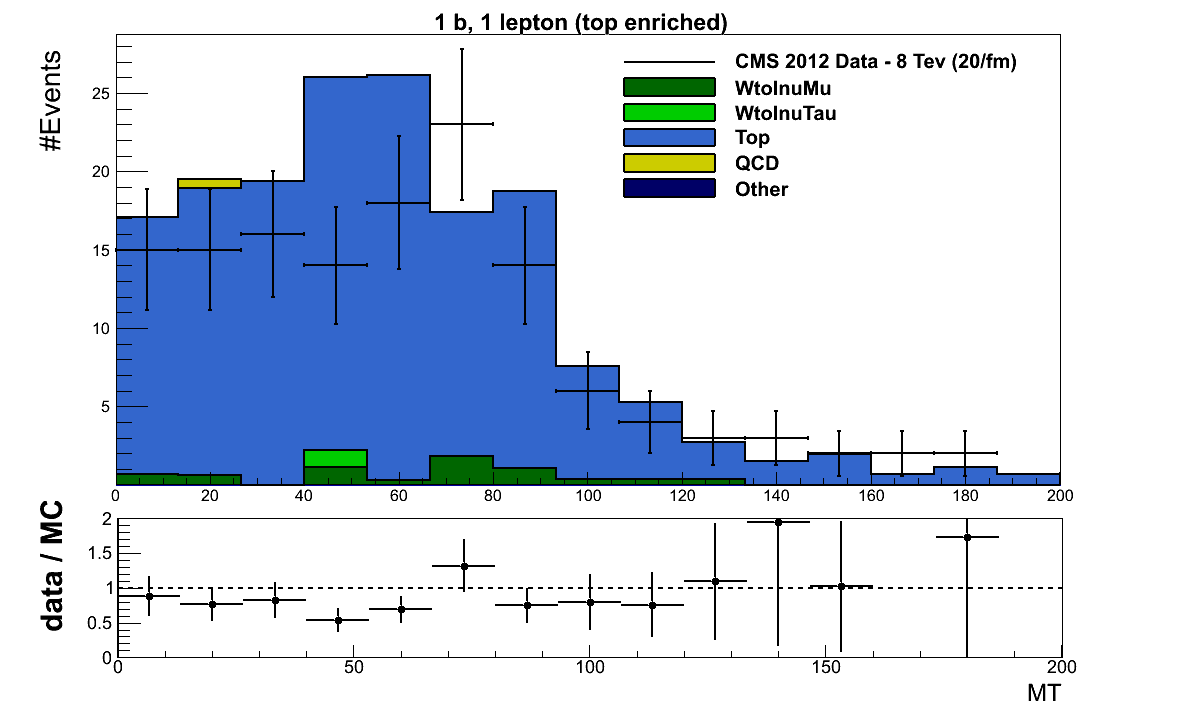
\includegraphics[angle=00,width=0.5\textwidth]{figs/MT_1b_Mod.png}\\
	\mbox{\small{(c)}}  \\
\end{array}$
\end{center}
\caption{Muon \pT, \mttwo and \mt distributions for top-enriched region}
\label{fig:topEnrichedPlots}
\end{figure}

%.....................
\begin{table}[!htb]
\setlength{\tabcolsep}{2pt}
\small
\begin{center} 

\begin{tabular}{lccccccccc} 
\hline\hline
& WtolnuMu& WtolnuTau& QCD& Zinv& Top& SMS& Other& MC& data \\ \hline \hline
 All events ($\rm jets\geq X$) & 170.32  & 267.04  & 493.27  & 270.57  & 1122.03  & 0.00 & 211.59  & 2534.83 +- 86.48 & 2510.00  \\ 
 %$Minimum DPhi(\met,jet) > 0.3$ & 40.56  & 65.36  & 146.80  & 65.29  & 328.56  & 0.06  & 50.78  & 697.35 $\pm$ 52.10 & 597.00  \\ 
 %HBHE noise veto & 40.56  & 65.36  & 146.80  & 65.29  & 328.56  & 0.06  & 50.78  & 697.35 $\pm$ 52.10 & 597.00  \\ 
 %$\met > 30GeV$ & 40.56  & 65.36  & 146.80  & 65.29  & 328.56  & 0.06  & 50.78  & 697.35 $\pm$ 52.10 & 597.00  \\ 
% $VectorSumPt < 70$ & 40.56  & 65.36  & 146.80  & 65.29  & 328.56  & 0.06  & 50.78  & 697.35 $\pm$ 52.10 & 597.00  \\ 
Analysis selection cuts & 170.32  & 267.04  & 493.27  & 270.57  & 1122.03  & 0.00 & 211.59  & 2534.83 +- 86.48 & 2510.00  \\ 

Lepton Veto & 170.32  & 248.45  & 490.77  & 270.43  & 913.06  & 0.00 & 109.45  & 2202.48 +- 85.20 & 2192.00  \\ 
Lepton Selection & 107.15  & 20.76  & 0.62  & 0.12  & 236.72  & 0.00 & 5.85  & 371.23 +- 15.38 & 329.00  \\ 
$m_T < 100\, \rm GeV$ & 97.37  & 20.36  & 0.62  & 0.06  & 206.08  & 0.00 & 5.85  & 330.34 +- 14.53 & 293.00  \\
$b$-jets Selection & 5.71  & 1.06  & 0.61  & 0.00  & 141.35  & 0.00 & 0.00  & 148.74 +- 10.24 & 119.00  \\  
\mttwo  100 - 150 GeV & 0.64  & 0.41  & 0.00  & 0.00  & 16.11  & 0.00 & 0.00  & 17.16 +- 3.47 & 28.00  \\ 
\mttwo  150 - 200 GeV & 0.31  & 0.34  & 0.61  & 0.00  & 53.26  & 0.00 & 0.00  & 54.53 +- 6.38 & 43.00  \\ 
\mttwo  200 - 275 GeV & 1.46  & 0.00  & 0.00  & 0.00  & 43.72  & 0.00 & 0.00  & 45.18 +- 5.64 & 26.00  \\ 
\mttwo  275 - 375 GeV & 1.94  & 0.00  & 0.00  & 0.00  & 24.37  & 0.00 & 0.00  & 26.30 +- 4.14 & 16.00  \\ 
\mttwo  375 - 500 GeV & 0.68  & 0.00  & 0.00  & 0.00  & 1.79  & 0.00 & 0.00  & 2.47 +- 1.17 & 3.00  \\ 
$\mttwo > 500 GeV$ & 0.69  & 0.30  & 0.00  & 0.00  & 1.30  & 0.00  & 0.00  & 2.29 +- 1.10 & 2.00  \\
\hline\hline 
\end{tabular} 
\caption{Yields for the top-enriched selection}
\label{tab:toEnrichyields}
\end{center} 
\end{table}


%...........................
\subsubsection{Z Estimation Results}
After finding the number of top events in the b-tag veto (W-enriched) region, it is subtracted from the number of W's of this region, derived from data, to obtain the correct number of $W\rightarrow\mu\nu$ events. Due to requesting one b-jet in the final state we need to have the number of W's in 1 b-tag region to be able to estimate the number of Z in this region. Therefore we must multiply the number of W's in b-tag veto region to $\frac{\epsilon(1b W)}{\epsilon(0b W)}$ to reach the number of W's in 1 b-tag region and this ratio is coming from MC and it is considered b-tag scale factor.   

\subsubsection{Systematic uncertainties}
\label{subsect:ZnnSyst}
The systematic uncertainty on $Z\to \nu\nu$ estimation has contributions from different sources, as can be seen in Equation~\ref{eq:ZinvEst}. There, the uncertainty on $R^{MC}$ is taken from simulation where it includes the uncertainties due to the PDF set and the k-factor [FIXME?] in Z and W bosons production rates. The uncertaintiy on the muon acceptance efficiency is derived from simulation, too. The muon selection efficiency ($\epsilon_{reco/iso}$) as well as its uncertainty are data-driven, obtained from the Tag\&Probe method. Another uncertainty in this estimation arises from the requirement of $m_T<100\,\rm GeV$ which is estimated from simulation.\\
For the $N_{W(\mu\nu)}$ in the analysis region with at least one b-tagged jet, the $N_{W(\mu\nu)}$ estimation in b-tag veto region is corrected with  the data-driven b-tagging and b-tag veto efficiencies. The uncertainties on these efficiencies are taken from data, accordingly.\\
Other than $t\bar{t}$, all backgrounds and their uncertainties are estimated from simulation in $N_{W(\mu\nu)}$ calculation. The $t\bar{t}$ contribution in W-enriched (b-tag veto) region is obtained using Equation~\ref{eq:topEst}. In this estimation, the uncertainties on b-tagging efficiencies are taken from data while the background uncertanties are derived from simulation. \\ 

The final estimation together with their uncertainties are summarized in Table~\ref{tab:ZinvFinalRes}.

\begin{table}[!htb]
\small
\setlength{\tabcolsep}{20pt} 
\begin{center} 
\begin{tabular}{lccccccc} 
\hline\hline
&                 &    MC                     & Data Estimation\\\hline \hline
& top  (0b, 1l)     & 27.85 $\pm$ 4.68             &18.73 $\pm$ 4.56 ( 1.72 (stat) $\pm$4.22 (syst) )\\
&  W   (0b, 1l)     & 69.67 $\pm$ 4.79            & 89.98 $\pm$ 13.71 ( 8.08 (stat) $\pm$ 11.08 (syst))\\ 
& Zinv (1b, 0l)           &  22.74 $\pm$ 0.84            &19.68 $\pm$ 8.09 ( 1.77 (stat) $\pm$7.89 (syst))\\


\hline\hline 
\end{tabular} 
\caption{Z-invisible Estimation}
\label{tab:ZinvFinalRes}
\end{center} 
\end{table}


\section[Statistics]{Statistical Interpretation of the results}\label{sect:stat}

Since no excess of data over the background prediction has been observed, 
we close our study with setting upper limits on the testing signals.
This is conducted using a modified frequentist approach, namely CLs method \cite{read:CLs}.
In this method, the test statistic $q_\mu$ \cite{cowan:asymptoticCLs} is a function of the profile likelihood-ratio,

\begin{align}
q_\mu = -2 \ln \frac{\mathcal{L}(data ;\, b + \mu s)}{\mathcal{L}(data ;\, b + \hat{\mu} s)},
\end{align}

where $\hat\mu$ is the \textit{signal strength modifier} $\mu$ at the maximum point of the likelihood $\mathcal{L}$.
Then CLs is given by the following probability-ratio,

\begin{align}
CL_s = \frac{p(q_\mu \geq q_\mu^{obs} | b + \mu s )}{p(q_\mu \geq q_\mu^{obs} | b)}.
\end{align}
 
We compute CLs using a software package provided by the CMS Higgs PAG \cite{higgspag:software}.
After incorporating systematic uncertainties, an observed CLs smaller than 0.05 for a signal strength of $\mu = 1$, excludes the given signal at $95\%$ CL. Indeed, the package determines which signal strength $\mu$ excludes the testing signal at $95\%$ CL. Therefore all resulting $\mu \leq 1$ define the excluded region in the parameter space of the given signal. 

In this study, we analyze data in 8 different bins (multi-bin analysis) to utilize more information from 
the observed and the predicted distributions.
%bins' contents of the observations and the predictions.
The bins are defined in reconstructed top quark multiplicity, zero or more. In addition, events are categorized based on the $\mttwo$ values: $125\rm{GeV} \leq \mttwo < 150\rm{GeV},\; 150\rm{GeV} \leq \mttwo < 200\rm{GeV},\; 200\rm{GeV} \leq \mttwo < 250\rm{GeV},\; 250\rm{GeV} \leq \mttwo < \infty$.
%These bins are determined, for an event, based on whether the event contents reconstructed top quarks or not (2 bins) times which bin of $\mttwo$ is occupied by the event (4 bins of $125\rm{GeV} \leq \mttwo < 150\rm{GeV},\; 150\rm{GeV} \leq \mttwo < 200\rm{GeV},\; 200\rm{GeV} \leq \mttwo < 250\rm{GeV},\; 250\rm{GeV} \leq \mttwo < \infty$). 

To investigate the exclusion power of our research, we study the topology of direct stop pair production  in Simplified Models \cite{alves:sms}, with $\tilde{t}\to \tilde{\chi}^0_1 t$ (T2tt). The research excludes a small region of the phase space around the point of ($m_{\tilde{t}} = 375\rm{GeV}$ and $ m_{LSP} = 50\rm{GeV}$) with an integrated luminosity of $5.1\,\invfb$. 
This region is too small, nevertheless the reasonable results in background estimations and using a different variable ($\mttwo$) from the other analysis groups motivates us to optimize the analysis with more integrated luminosity ($20\,\invfb$) in order to extend reach of the tested signal. 

Figure \ref{fig:limit_20inf} shows the expected upper limit on the cross section of the stop pair production in terms of Simplified Models. 
Furthermore, the figure shows the expected exclusion power considering $30\%, 40\%$ and $50\%$ systematic uncertainties on signal and background rates which are predicted using Monte-Carlo simulations. The black curve represents the observed reach by the common Cut$\&$Count search using $\met$ trigger. As the figure shows this analysis can be 
comparable with other analyses and with even more optimized search, it has the potential to be complementary to other analyses in some regions of the phase space.  

%%%%%%%%%%
\begin{linenomath}
\begin{figure}[h]
\centering
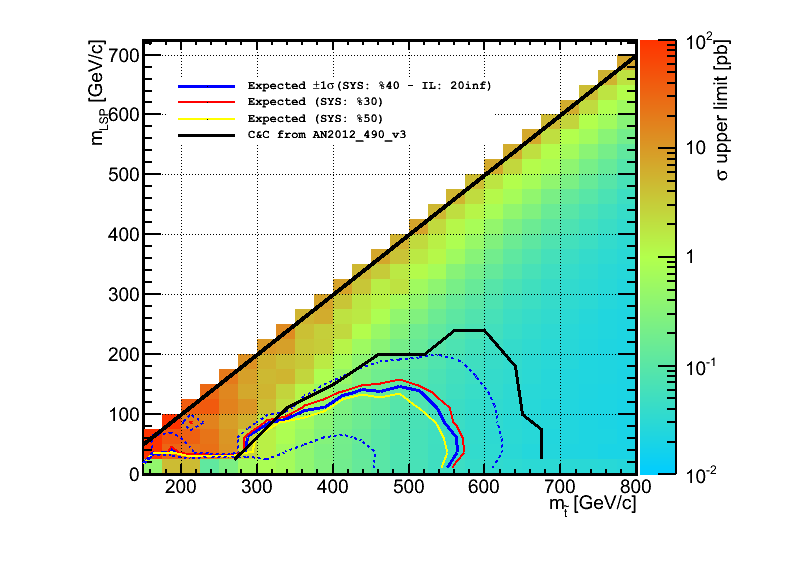
\includegraphics[width=0.7\textwidth,keepaspectratio=true]{StatisticsFig/limit_304050sys_20inf_20130625.png}
\caption{Expected exclusion power in terms of Simplified Models (T2tt-topology) with an integrated luminosity of $20\,\invfb$. Backgrounds are predicted using Monte-Carlo simulations and a rough estimate of systematic uncertainties equal $30\%, 40\%$ and $50\%$ are taken into account.}
\label{fig:limit_20inf}
\end{figure}
\end{linenomath}
%%%%%%%%%%


%%%%%%%%%%
%\begin{linenomath}
%\begin{figure}[h]
%\centering
%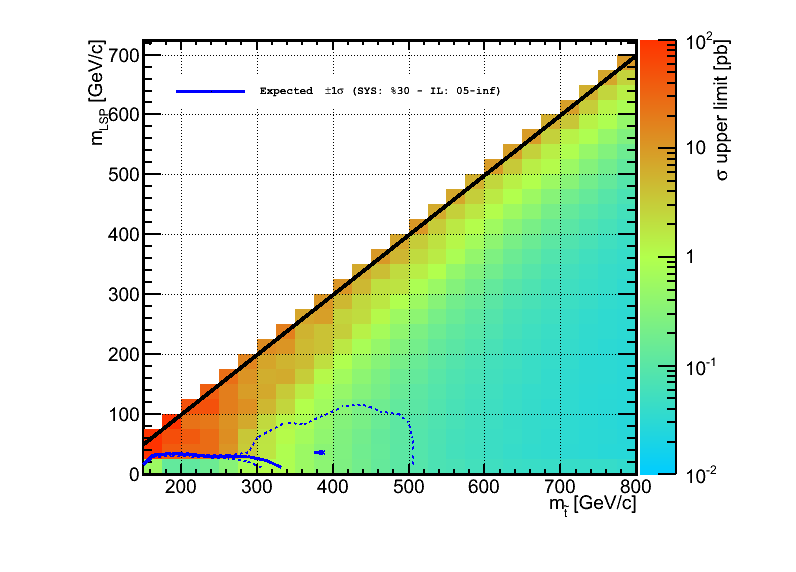
\includegraphics[width=0.7\textwidth,keepaspectratio=true]{StatisticsFig/limit_30sys_05inf_20130625.png}
%\caption{}
%\label{fig:limit_05inf}
%\end{figure}
%\end{linenomath}
%%%%%%%%%%

%%%%%%%%%%
%\begin{linenomath}
%\begin{figure}[h]
%\centering
%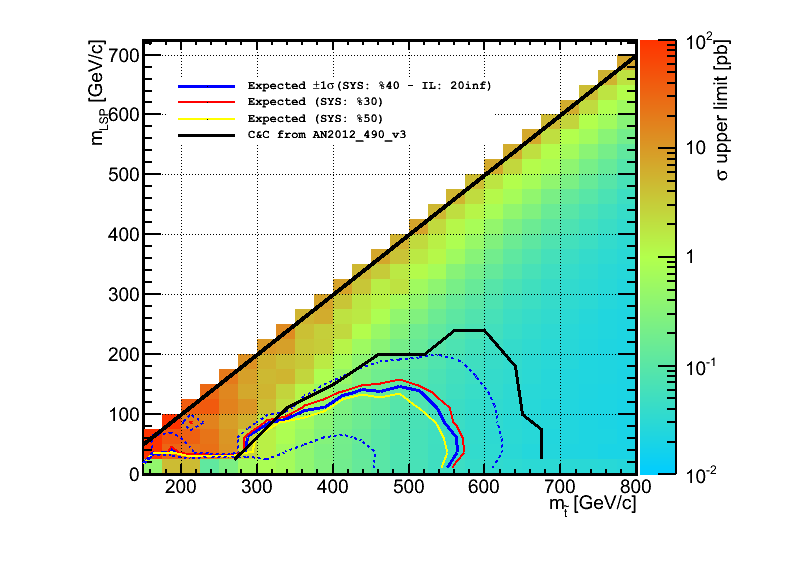
\includegraphics[width=0.7\textwidth,keepaspectratio=true]{StatisticsFig/limit_304050sys_20inf_20130625.png}
%\caption{}
%\label{fig:limit_20inf}
%\end{figure}
%\end{linenomath}
%%%%%%%%%%


\section{Conclusion}
\label{sect:conclusion}
A hadronic search for direct Stop production is presented using the \mttwo variable. Data driven methods are used to estimate the main
backgrounds. It is shown that the methods close properly on MC. Since this analysis uses a multijet trigger and \mttwo does not 
depend explicitly on \met, this analysis can be complementary to the common cut and count search for Stop which uses \met trigger. 
It is shown that in the regions with low mass difference between $m_{\tilde{t}}$ and 
$m_{LSP}$ this analysis can have a comparable reach. There is a plan to optimize the cuts to improve the reach in this region and exclude the
masses which are not reachable by the other analyses.

\section{Outlook of the Analysis}
In next step, the analysis will be updated to the full dataset of 2012 which sums up to about 20 \invfb of data. 
There is an idea to look at the "Parked data" also. Thanks to the looser triggers in the "Parked data", 
it is expected to have a better signal efficiency when the analysis applied on this data. 
Re-optimizing the analysis with these looser triggers is foreseen for next steps to improve the reach even further.

\section{Acknowledgements}
This analysis benefits highly from the computing resources and codes developed in ETHZurich. 
We appreciate their help and generosity. The method used for the top reconstruction was firstly introduced and implemented by L. Pape. 
We thank him for providing us the code. The authors would like to thank the conveners of the SUSY-TBT working group, Rick Cavanaugh 
and Juan Alcaraz Maestre, for their help and support. The authors would like to thank the management and staff of the school of particles 
and accelerators of IPM, especially Prof. Arfaei for their help and support. Thanks to all of the members of
the CMS collaboration for their outstanding results discussed partly here.

\bibliography{auto_generated}
%%% DO NOT ADD \end{document}!

